% =========================
% Paper 2 - Work in Progress
% Dynamical Flow Analysis: MCI, AD, and Healthy Controls
% Plus MCI Subtype Stratification
% =========================

\documentclass[5p,twocolumn,authoryear]{elsarticle}

\usepackage{natbib}
\biboptions{authoryear,round}
\usepackage{amsmath,amssymb}
\usepackage{graphicx}
\usepackage{hyperref}
\usepackage{booktabs}
\usepackage{float}
\usepackage{placeins}
\usepackage{caption}
\usepackage{subcaption}

% Helper macros
\newcommand{\figref}[1]{Fig.~\ref{#1}}
\newcommand{\tabref}[1]{Table~\ref{#1}}
\newcommand{\secref}[1]{Sec.~\ref{#1}}

\journal{Technical Report}

\begin{document}

\begin{frontmatter}

\title{Dynamical Flow Analysis of Resting-State EEG in MCI, Alzheimer's Disease, and Healthy Controls: Results Report}

\author[1]{\L{}ukasz Furman}

\address[1]{Faculty of Physics, Astronomy and Informatics, Nicolaus Copernicus University, 87-100, Toru\'{n}, Poland}

\begin{abstract}
This report presents preliminary results from applying the dynamical microscope framework to resting-state EEG data from Healthy Controls (HC), Mild Cognitive Impairment (MCI), and Alzheimer's Disease (AD) participants. We analyze latent trajectory dynamics using flow metrics computed in PCA-reduced autoencoder latent space. Additionally, we examine MCI subtype stratification based on MMSE severity and functional impairment scores. Key findings include: (1) large effect sizes for Speed CV, Occupancy Entropy, and Path Tortuosity distinguishing HC from MCI; (2) Explored Variance shows significant differences between HC and both clinical groups; (3) MCI subtypes show differential flow patterns based on cognitive severity.
\end{abstract}

\begin{keyword}
Resting-state EEG \sep MCI \sep Alzheimer's disease \sep dynamical systems \sep flow metrics \sep subtype analysis
\end{keyword}

\end{frontmatter}

% =========================
\section{Methods Summary}
% =========================

\subsection{Dataset}

The Greek Resting-State EEG dataset comprises recordings from three groups:
\begin{itemize}
    \item \textbf{Healthy Controls (HC)}: $n = 30$
    \item \textbf{Mild Cognitive Impairment (MCI)}: $n = 30$
    \item \textbf{Alzheimer's Disease (AD)}: $n = 30$
\end{itemize}

For the MCI subtype analysis, we used $n = 82$ MCI participants with available clinical metadata (MMSE scores and functional impairment ratings).

\subsection{Dynamical Microscope Pipeline}

The analysis follows the dynamical microscope framework:
\begin{enumerate}
    \item \textbf{Phase-amplitude encoding}: Multichannel EEG converted to circular phase--amplitude features using Hilbert transform.
    \item \textbf{Autoencoder latent space}: A ConvLSTM autoencoder learns a 64-dimensional latent representation of ongoing EEG dynamics.
    \item \textbf{Dimensionality reduction}: PCA projection to 2D for visualization and flow field estimation.
    \item \textbf{Flow metrics}: Trajectory-based metrics computed in both full latent space and 2D projections.
\end{enumerate}

\subsection{Flow Metrics}

We compute the following metrics per subject:
\begin{itemize}
    \item \textbf{Mean Speed}: Average velocity through latent space
    \item \textbf{Speed CV}: Coefficient of variation capturing dynamics variability
    \item \textbf{N Dwell Episodes}: Number of low-speed dwelling periods
    \item \textbf{Occupancy Entropy}: Entropy of spatial occupancy distribution
    \item \textbf{Path Tortuosity}: Ratio of path length to displacement (path complexity)
    \item \textbf{Explored Variance}: Total variance of trajectory in latent space
\end{itemize}

Bootstrap resampling ($n = 500$) provides 95\% confidence intervals for all metrics.

% =========================
\section{Results: HC vs MCI vs AD}
\label{sec:hc_mci_ad}
% =========================

\subsection{Bootstrap Metrics Overview}

\figref{fig:bootstrap_metrics} presents the bootstrap distributions of flow metrics across the three diagnostic groups.

\begin{figure}[H]
    \centering
    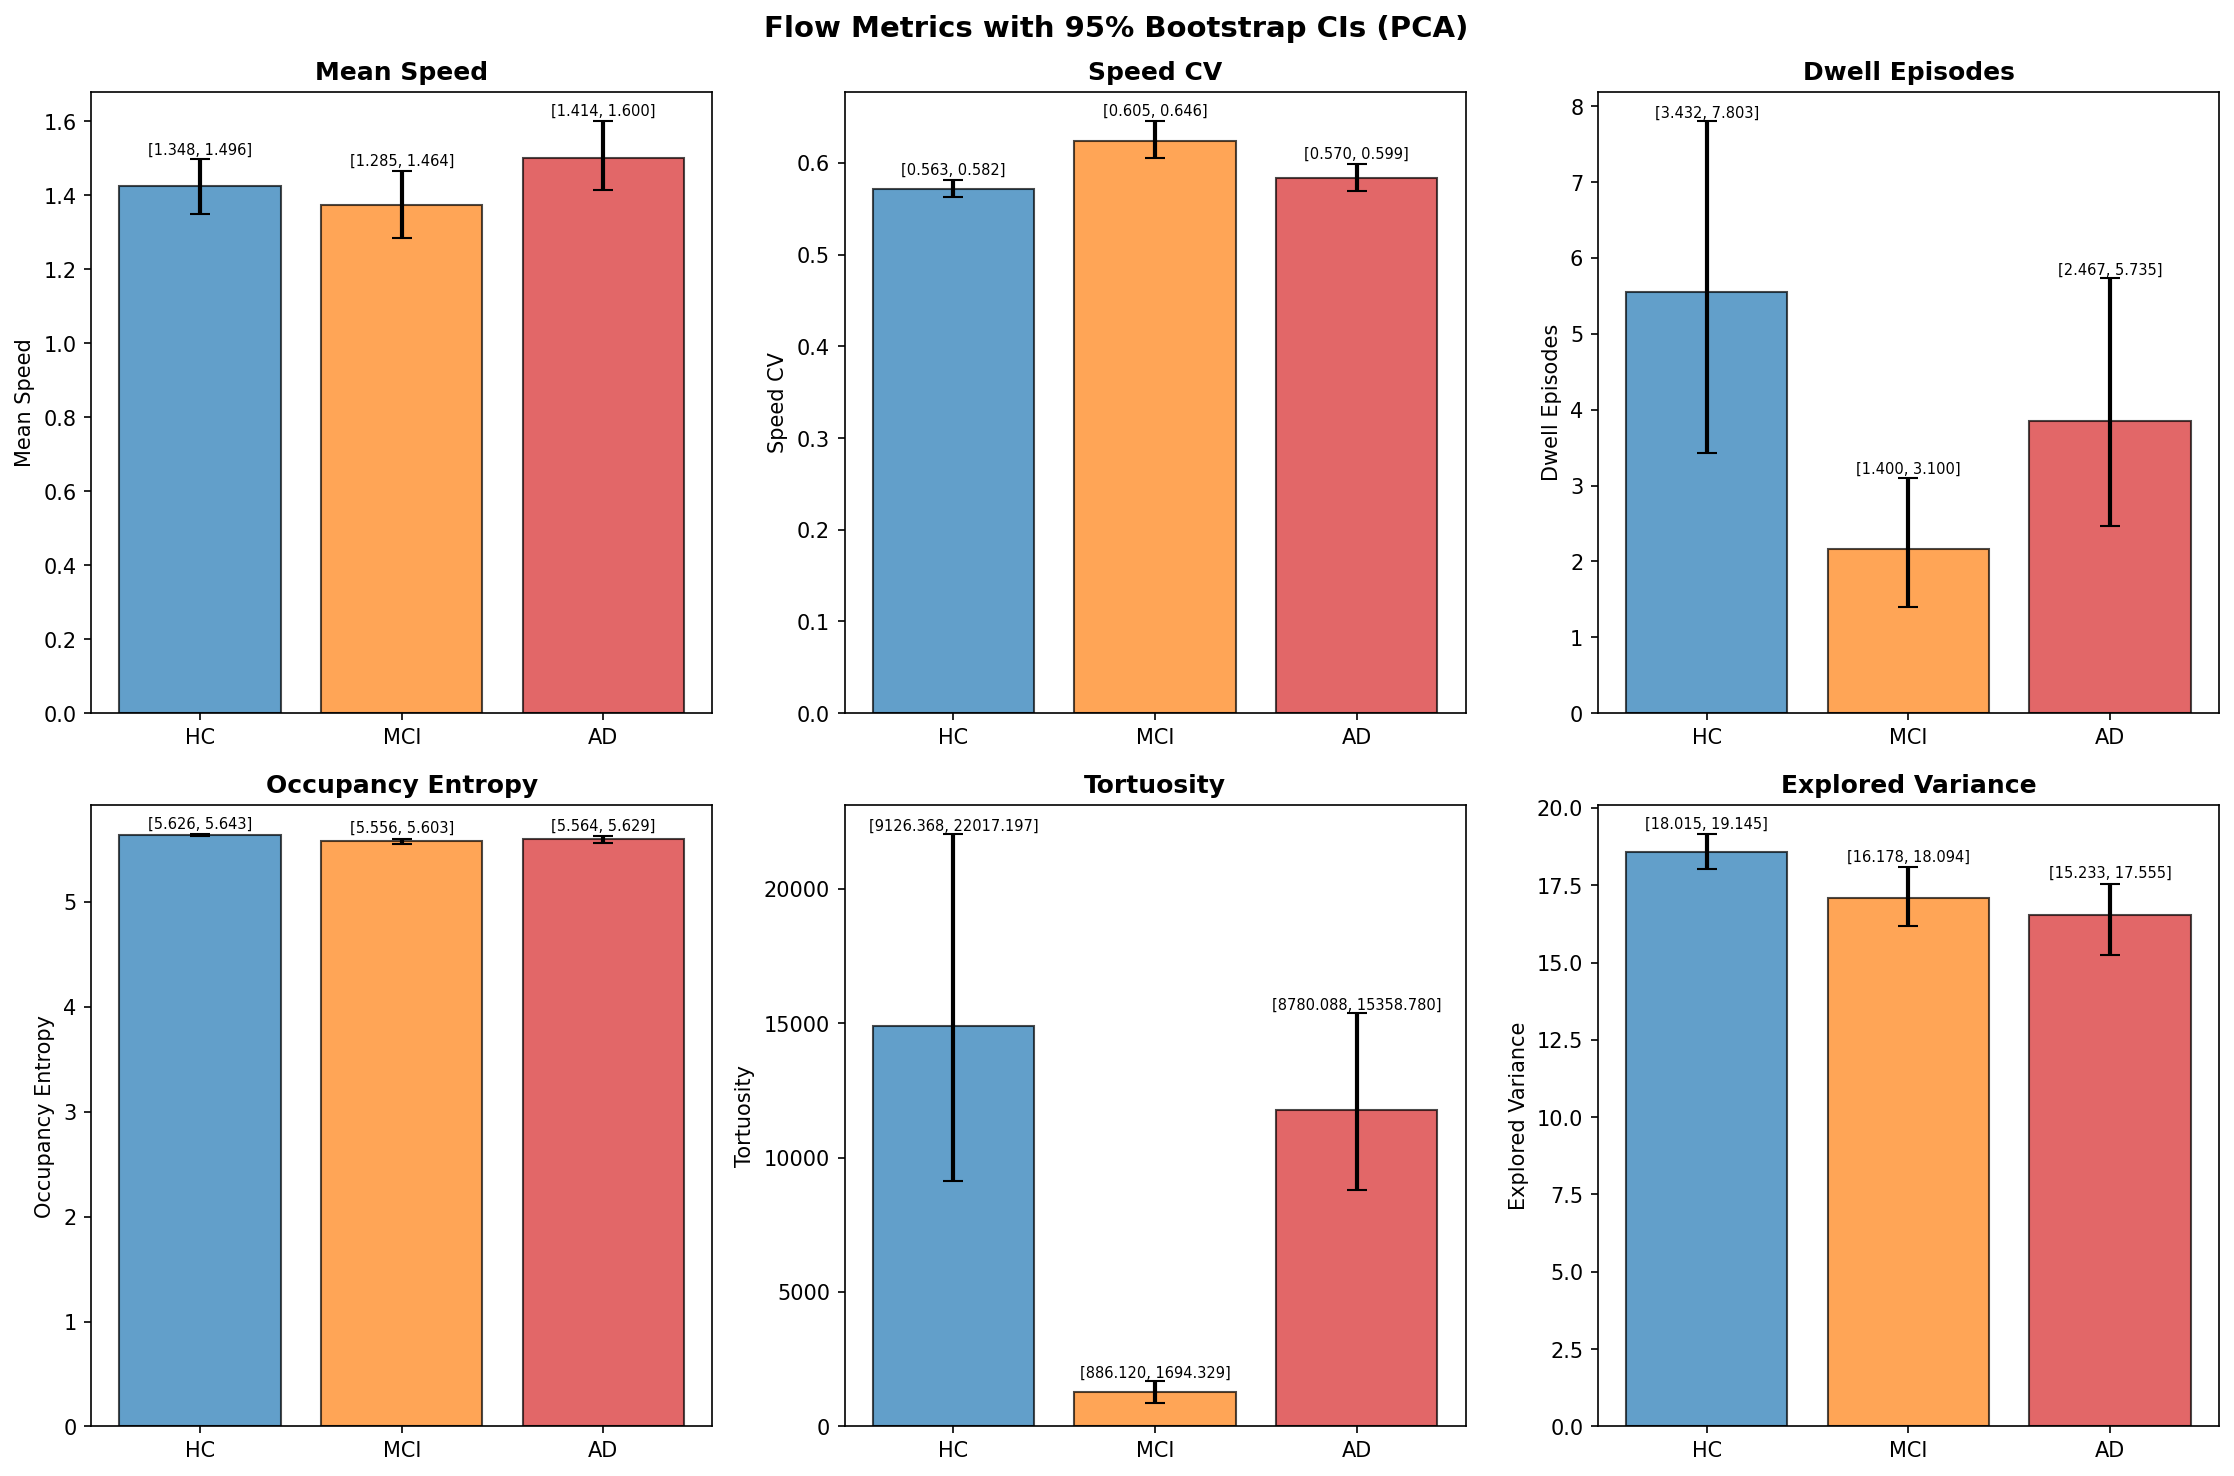
\includegraphics[width=\linewidth]{figures/paper2-wip/bootstrap_metrics_pca.png}
    \caption{Bootstrap distributions of flow metrics for HC, MCI, and AD groups. Violin plots show the distribution of bootstrap means with 95\% CI indicated.}
    \label{fig:bootstrap_metrics}
\end{figure}

\tabref{tab:summary_metrics} summarizes the metric values with bootstrap confidence intervals.

\begin{table}[H]
\centering
\caption{Flow Metrics with Bootstrap 95\% CIs by Diagnostic Group}
\label{tab:summary_metrics}
\begin{tabular}{lccc}
\toprule
Metric & HC & MCI & AD \\
\midrule
Mean Speed & 1.42 [1.35, 1.50] & 1.37 [1.28, 1.46] & 1.50 [1.41, 1.60] \\
Speed CV & 0.57 [0.56, 0.58] & 0.62 [0.61, 0.65] & 0.58 [0.57, 0.60] \\
N Dwell Episodes & 5.5 [3.4, 7.8] & 2.2 [1.4, 3.1] & 3.8 [2.5, 5.7] \\
Occupancy Entropy & 5.64 [5.63, 5.64] & 5.58 [5.56, 5.60] & 5.60 [5.56, 5.63] \\
Path Tortuosity & 14908 [9126, 22017] & 1269 [886, 1694] & 11753 [8780, 15359] \\
Explored Variance & 18.6 [18.0, 19.1] & 17.1 [16.2, 18.1] & 16.5 [15.2, 17.6] \\
\bottomrule
\end{tabular}
\end{table}

\subsection{Effect Sizes}

\figref{fig:effect_sizes} shows Cohen's $d$ effect sizes for pairwise group comparisons.

\begin{figure}[H]
    \centering
    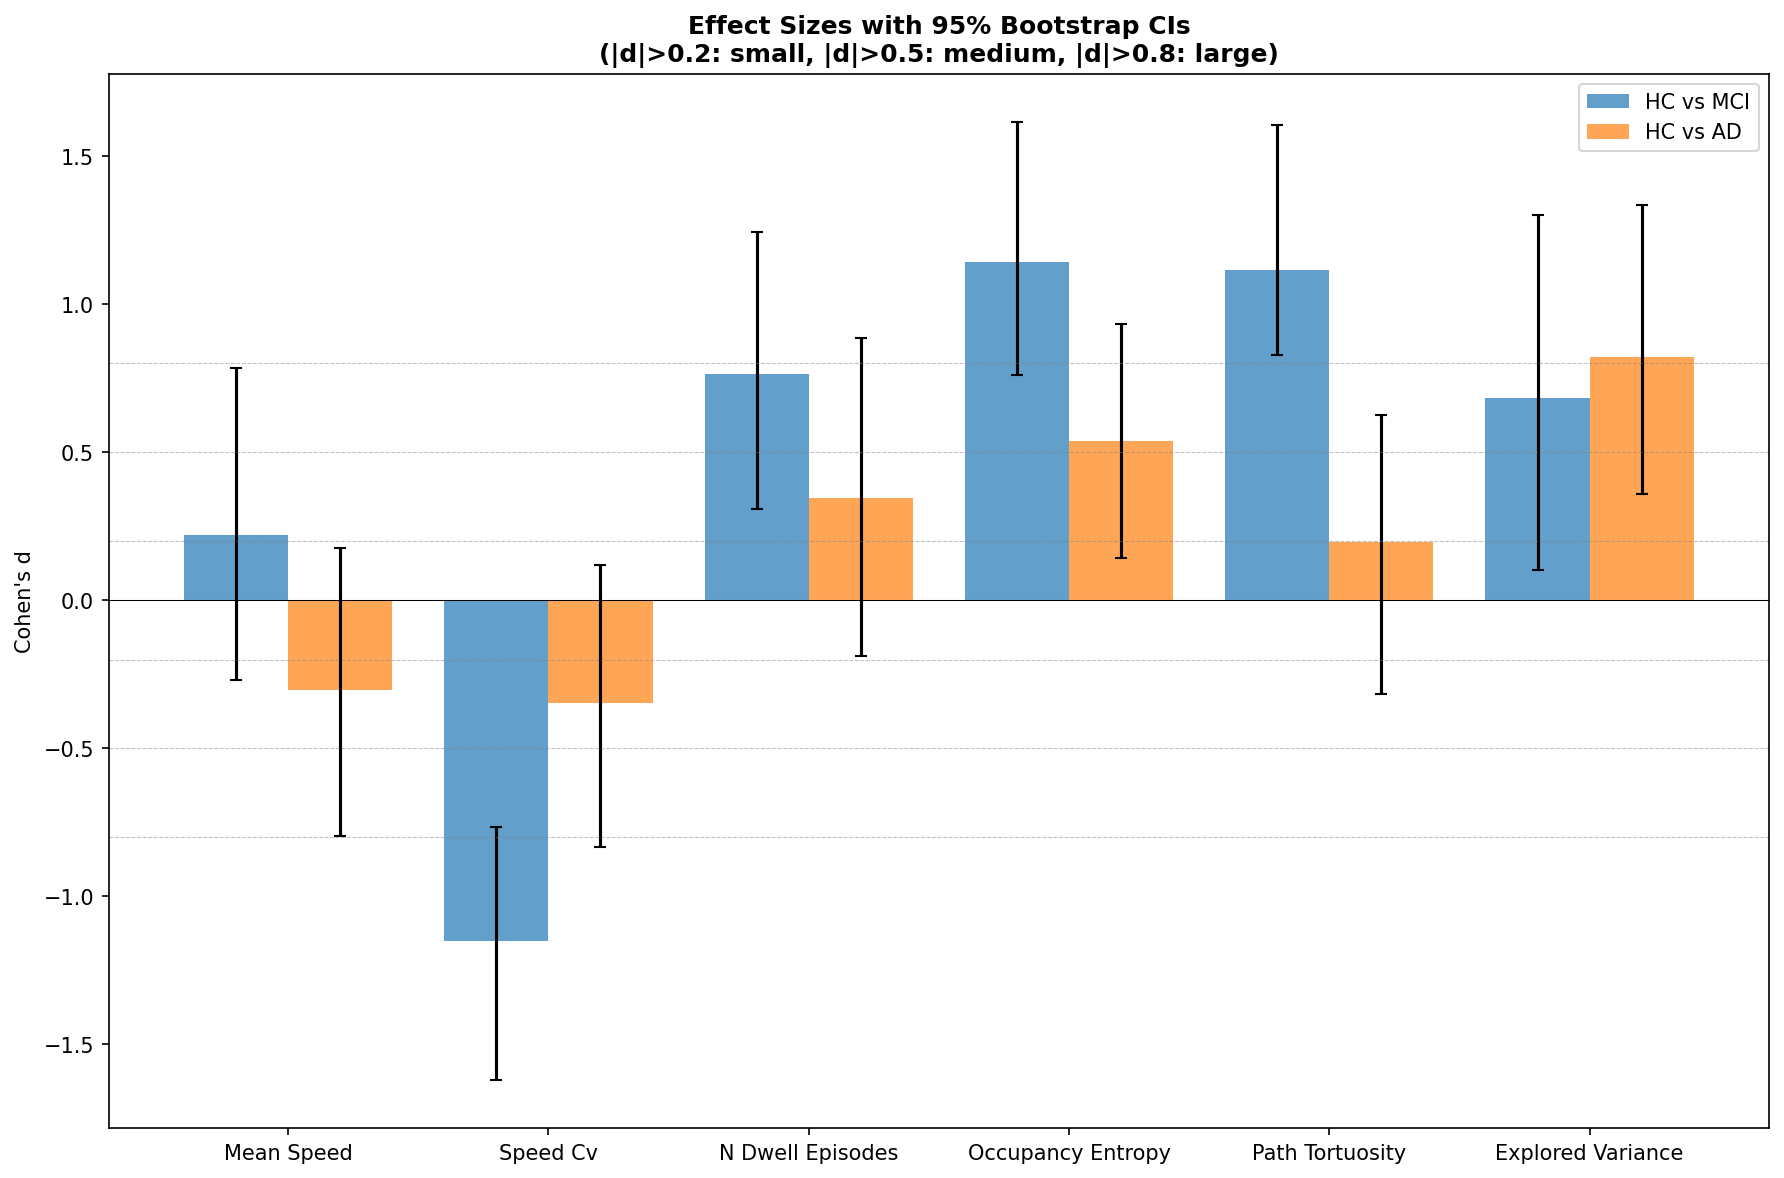
\includegraphics[width=\linewidth]{figures/paper2-wip/effect_sizes.png}
    \caption{Effect sizes (Cohen's $d$) with 95\% bootstrap CIs for HC vs MCI and HC vs AD comparisons across flow metrics.}
    \label{fig:effect_sizes}
\end{figure}

\textbf{HC vs MCI} comparisons reveal:
\begin{itemize}
    \item \textbf{Speed CV}: $d = -1.15$ [-1.62, -0.76] --- \textbf{large effect}, MCI shows higher variability
    \item \textbf{Occupancy Entropy}: $d = 1.14$ [0.76, 1.62] --- \textbf{large effect}, HC explores more uniformly
    \item \textbf{Path Tortuosity}: $d = 1.11$ [0.83, 1.60] --- \textbf{large effect}, MCI shows less complex paths
    \item \textbf{N Dwell Episodes}: $d = 0.76$ [0.31, 1.24] --- \textbf{medium effect}
    \item \textbf{Explored Variance}: $d = 0.68$ [0.10, 1.30] --- \textbf{medium effect}
\end{itemize}

\textbf{HC vs AD} comparisons show:
\begin{itemize}
    \item \textbf{Explored Variance}: $d = 0.82$ [0.36, 1.34] --- \textbf{large effect}
    \item \textbf{Occupancy Entropy}: $d = 0.54$ [0.14, 0.93] --- \textbf{medium effect}
    \item Other metrics show small or negligible effects
\end{itemize}

\textbf{Key observation}: MCI shows the strongest differentiation from HC on dynamics-related metrics (Speed CV, Path Tortuosity), while AD shows more similarity to HC on these measures but reduced Explored Variance.

\subsection{Density Difference Maps}

\figref{fig:density_diff_mci} and \figref{fig:density_diff_ad} show spatial density difference maps with confidence intervals.

\begin{figure}[H]
    \centering
    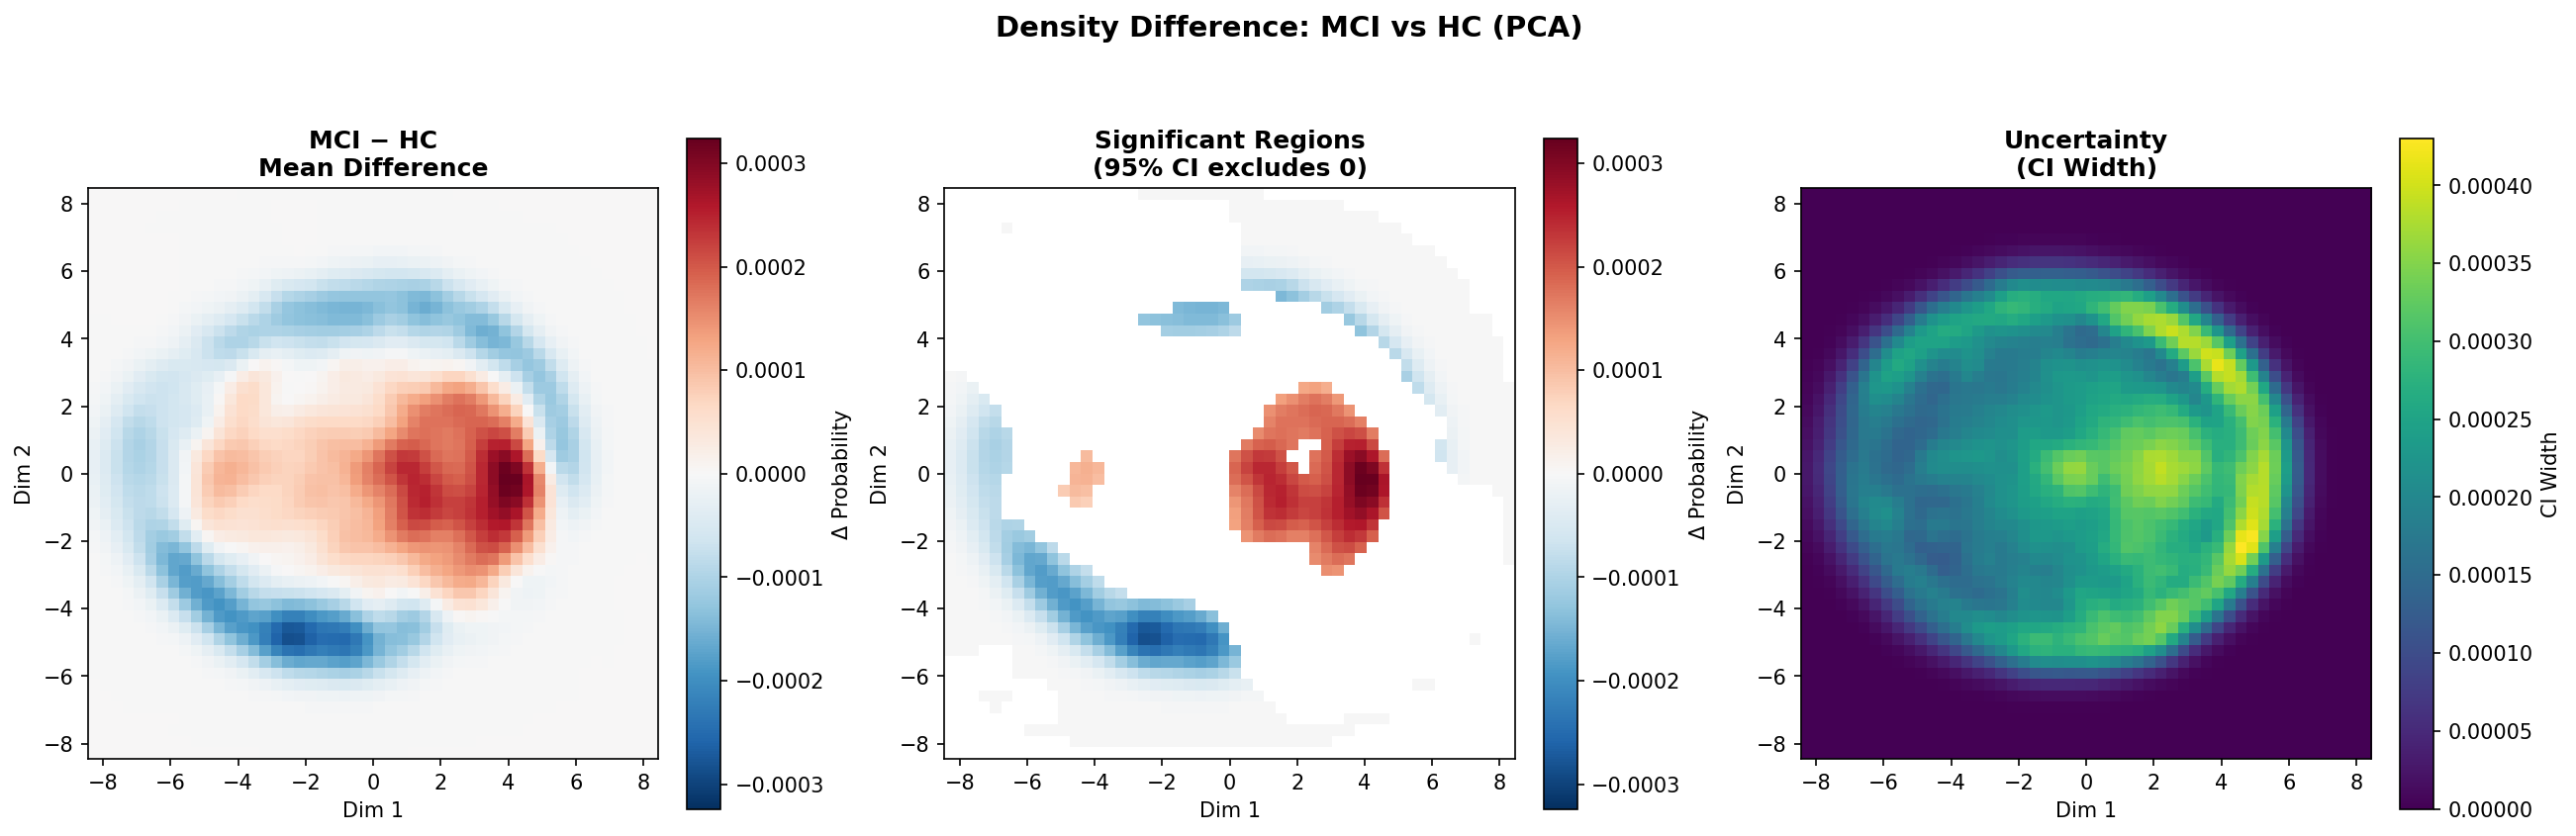
\includegraphics[width=\linewidth]{figures/paper2-wip/density_diff_ci_mci_pca.png}
    \caption{Density difference map: MCI vs HC. Warm colors indicate regions where MCI has higher occupancy; cool colors indicate HC-dominant regions. Hatching indicates non-significant differences.}
    \label{fig:density_diff_mci}
\end{figure}

\begin{figure}[H]
    \centering
    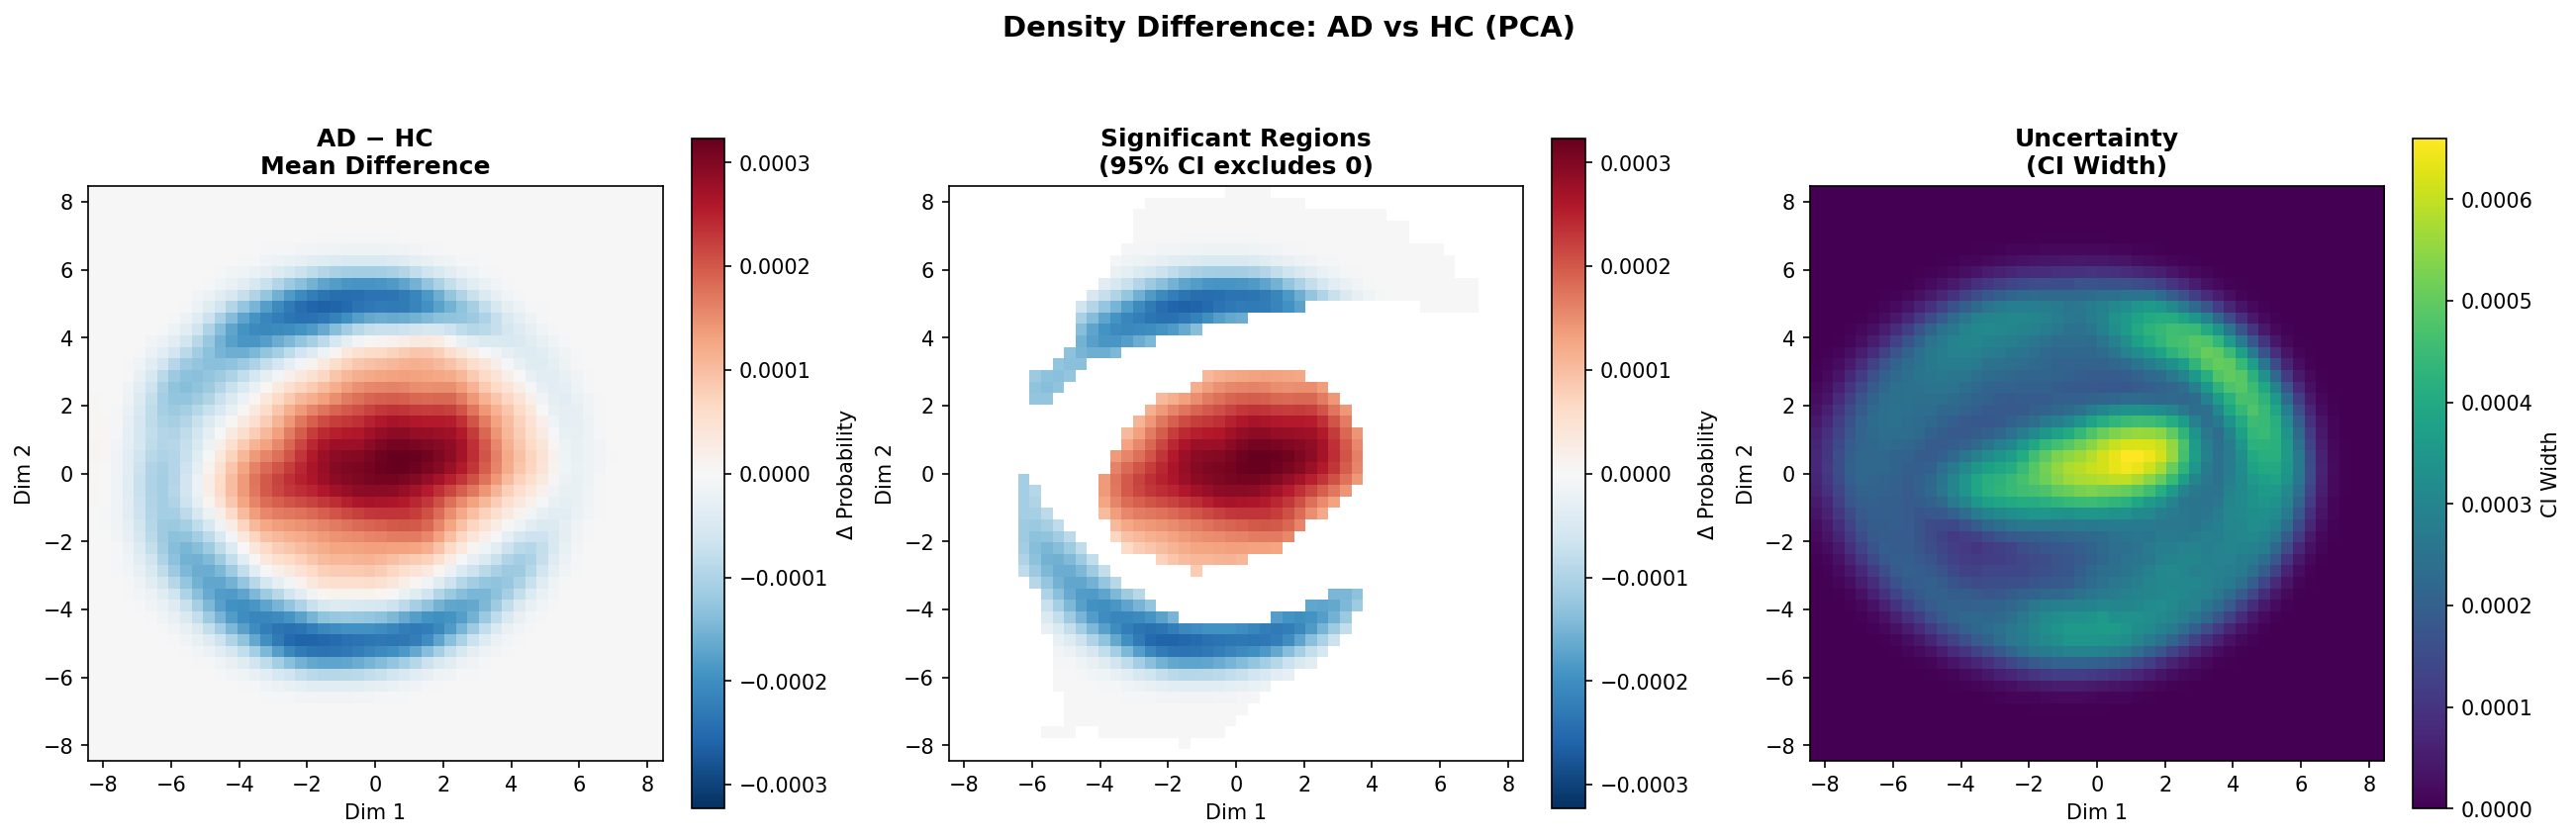
\includegraphics[width=\linewidth]{figures/paper2-wip/density_diff_ci_ad_pca.png}
    \caption{Density difference map: AD vs HC. Same conventions as \figref{fig:density_diff_mci}.}
    \label{fig:density_diff_ad}
\end{figure}

\subsection{Flow Field Analysis}

\figref{fig:group_flow_fields} presents the group-wise flow fields showing the average direction and magnitude of latent trajectory motion.

\begin{figure}[H]
    \centering
    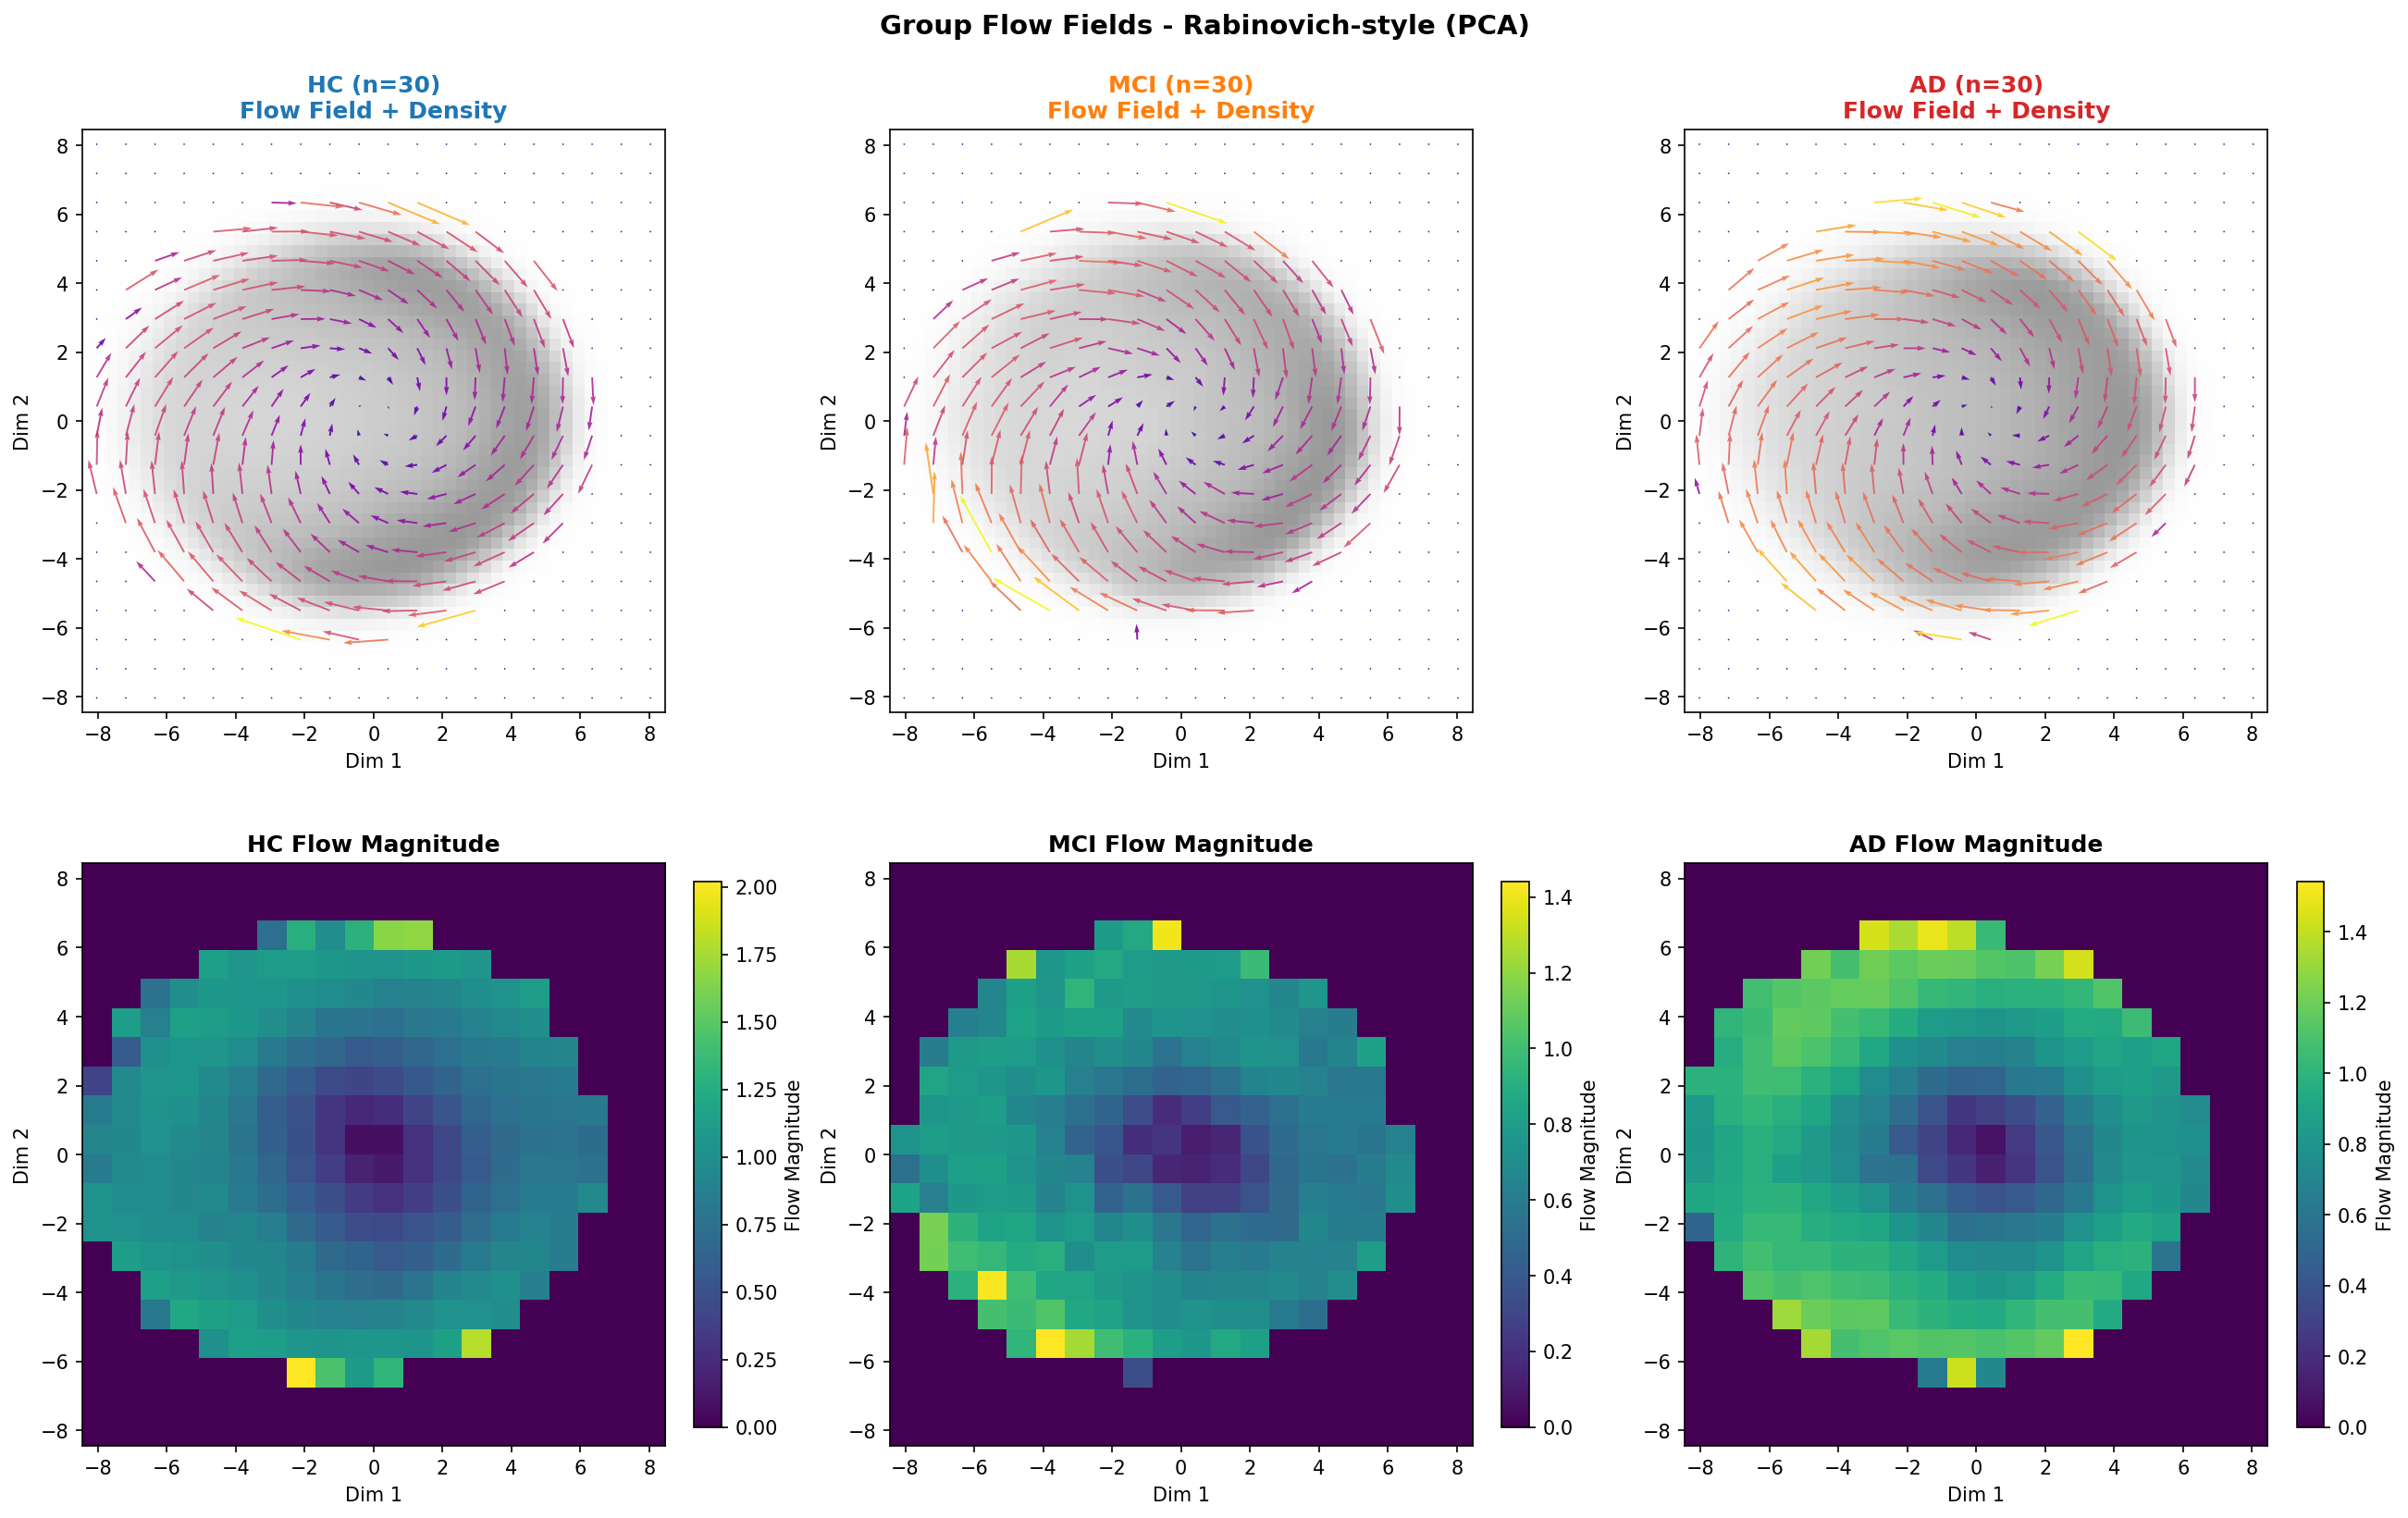
\includegraphics[width=\linewidth]{figures/paper2-wip/group_flow_fields_pca.png}
    \caption{Flow fields for HC, MCI, and AD groups. Arrow direction indicates mean flow direction; color/length indicates magnitude. Background shows occupancy density.}
    \label{fig:group_flow_fields}
\end{figure}

\figref{fig:flow_difference} shows the flow field difference between groups.

\begin{figure}[H]
    \centering
    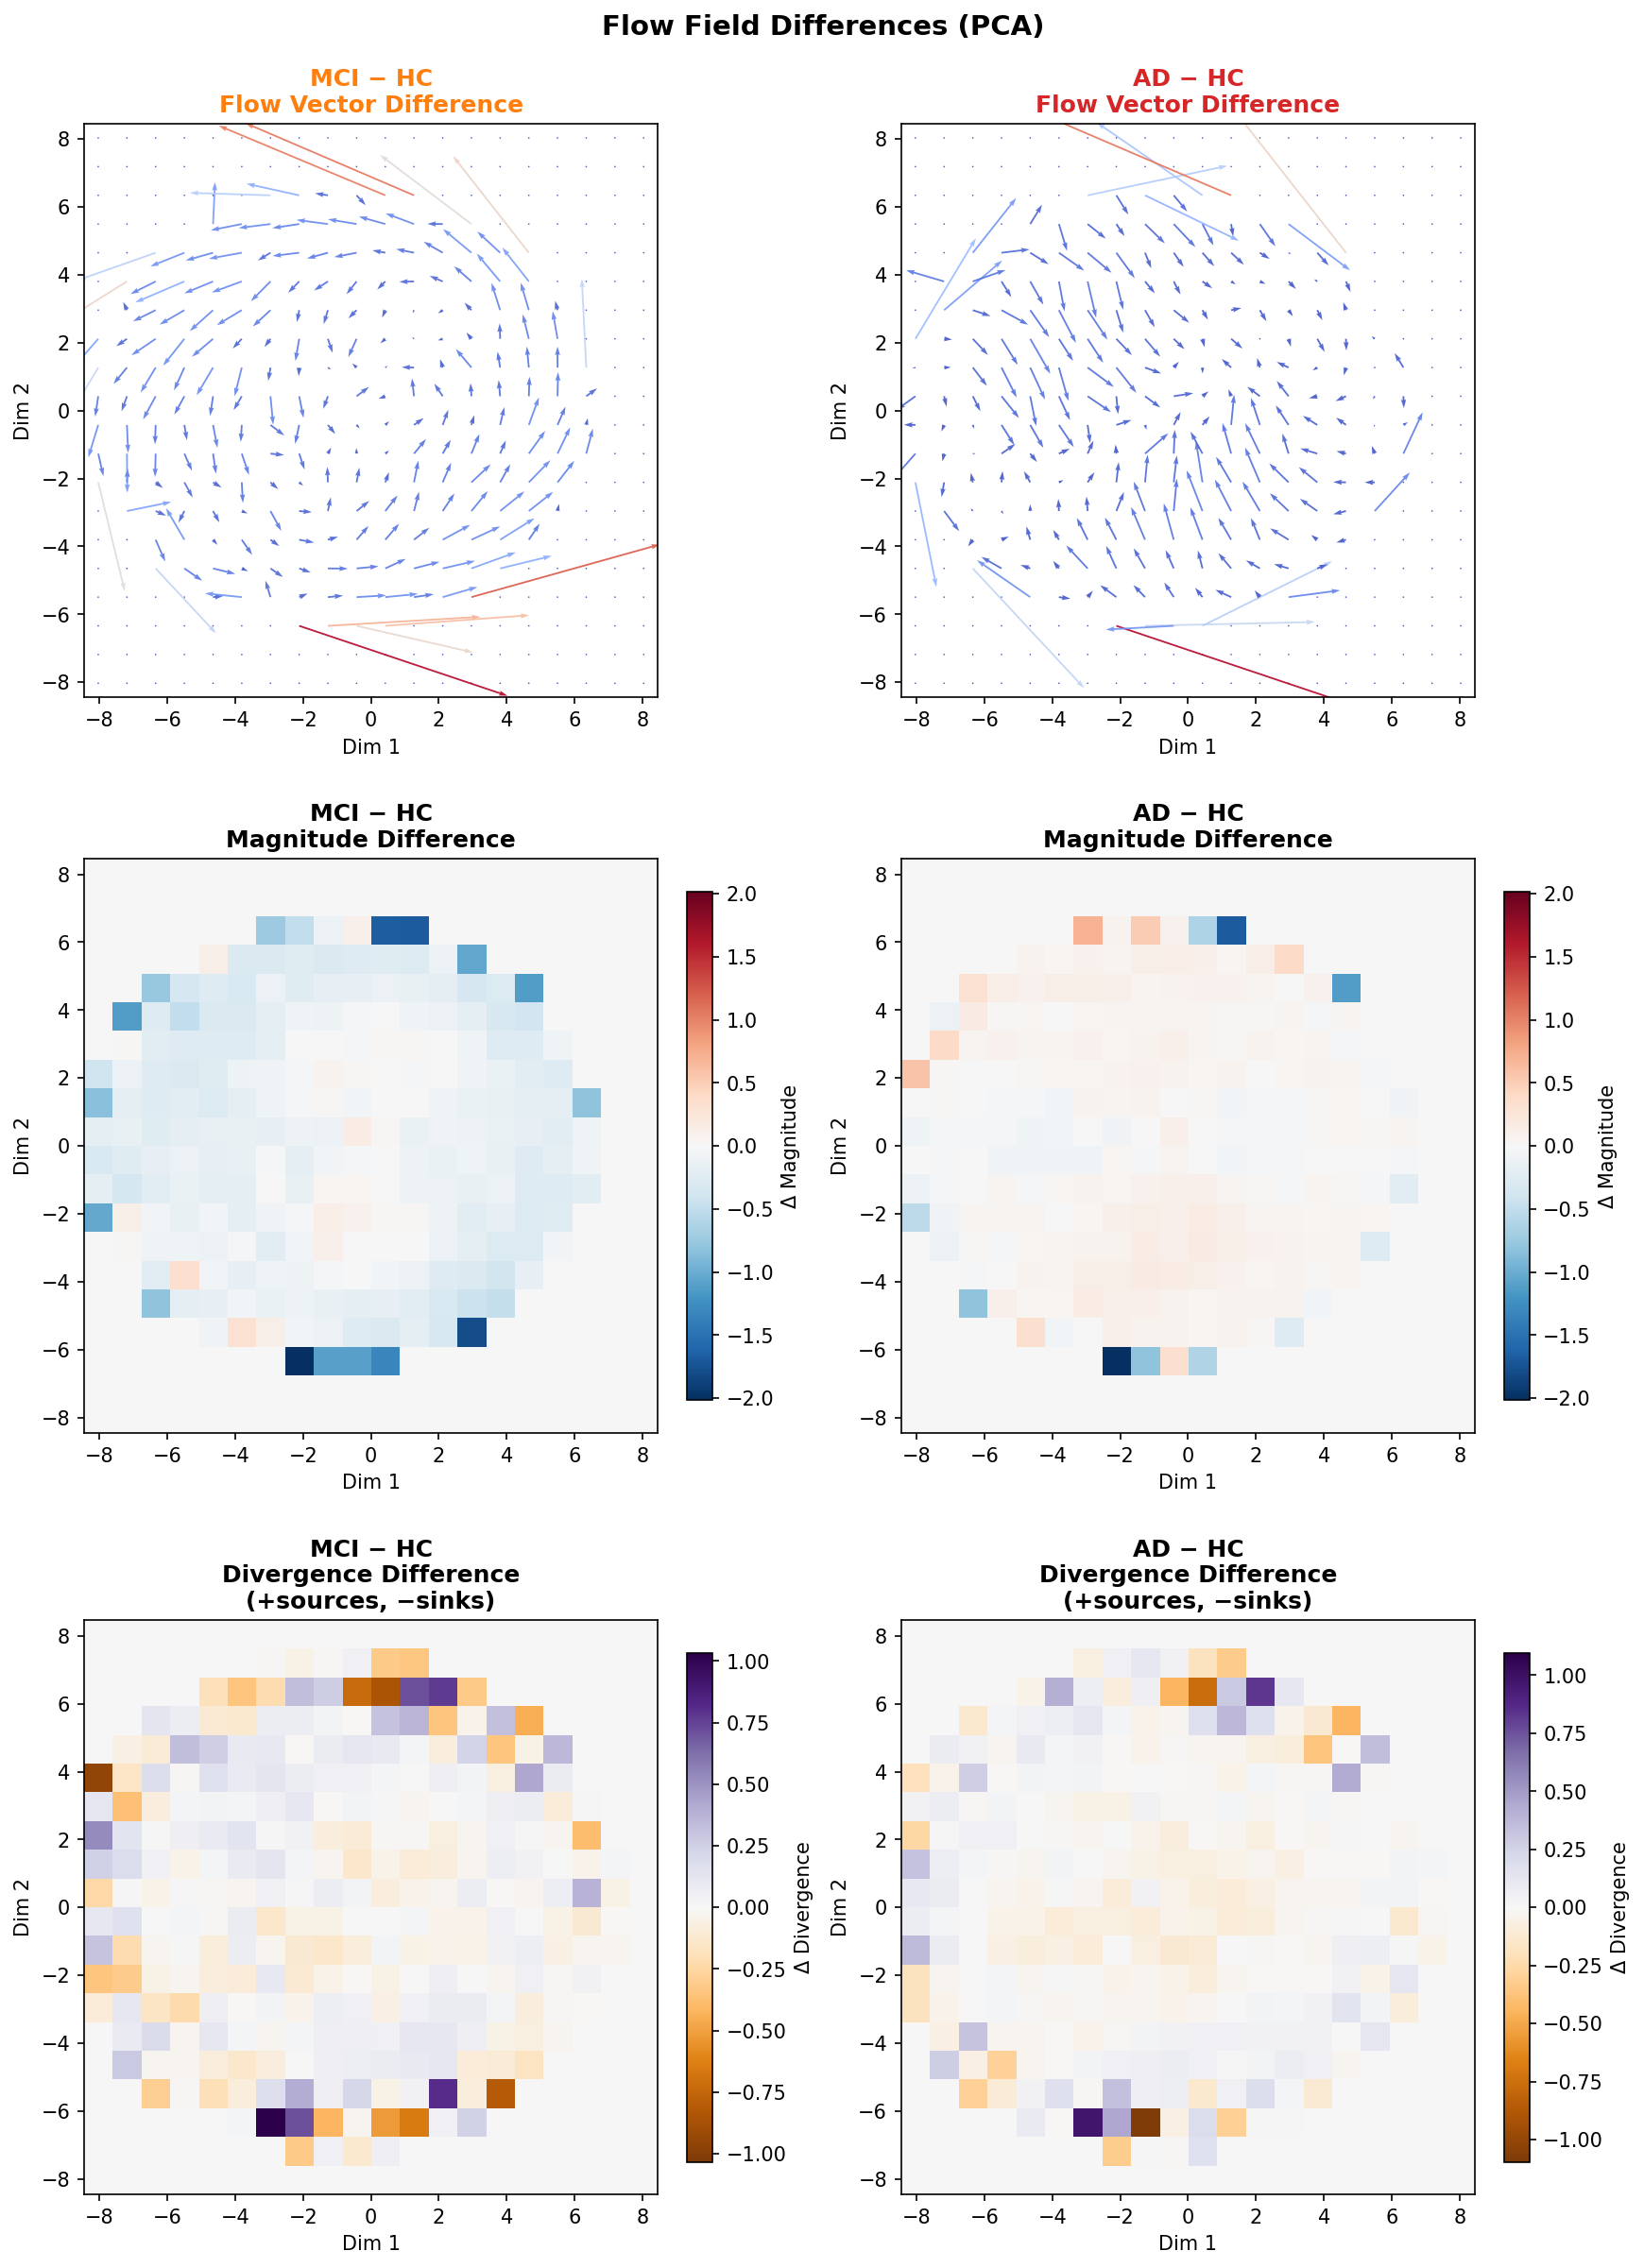
\includegraphics[width=\linewidth]{figures/paper2-wip/flow_difference_pca.png}
    \caption{Flow field differences between diagnostic groups. Top row: magnitude differences. Bottom row: divergence differences indicating expansion/contraction of flow.}
    \label{fig:flow_difference}
\end{figure}

\subsection{Radial Profiles}

\figref{fig:radial_profiles} shows how metrics vary as a function of distance from the latent space centroid.

\begin{figure}[H]
    \centering
    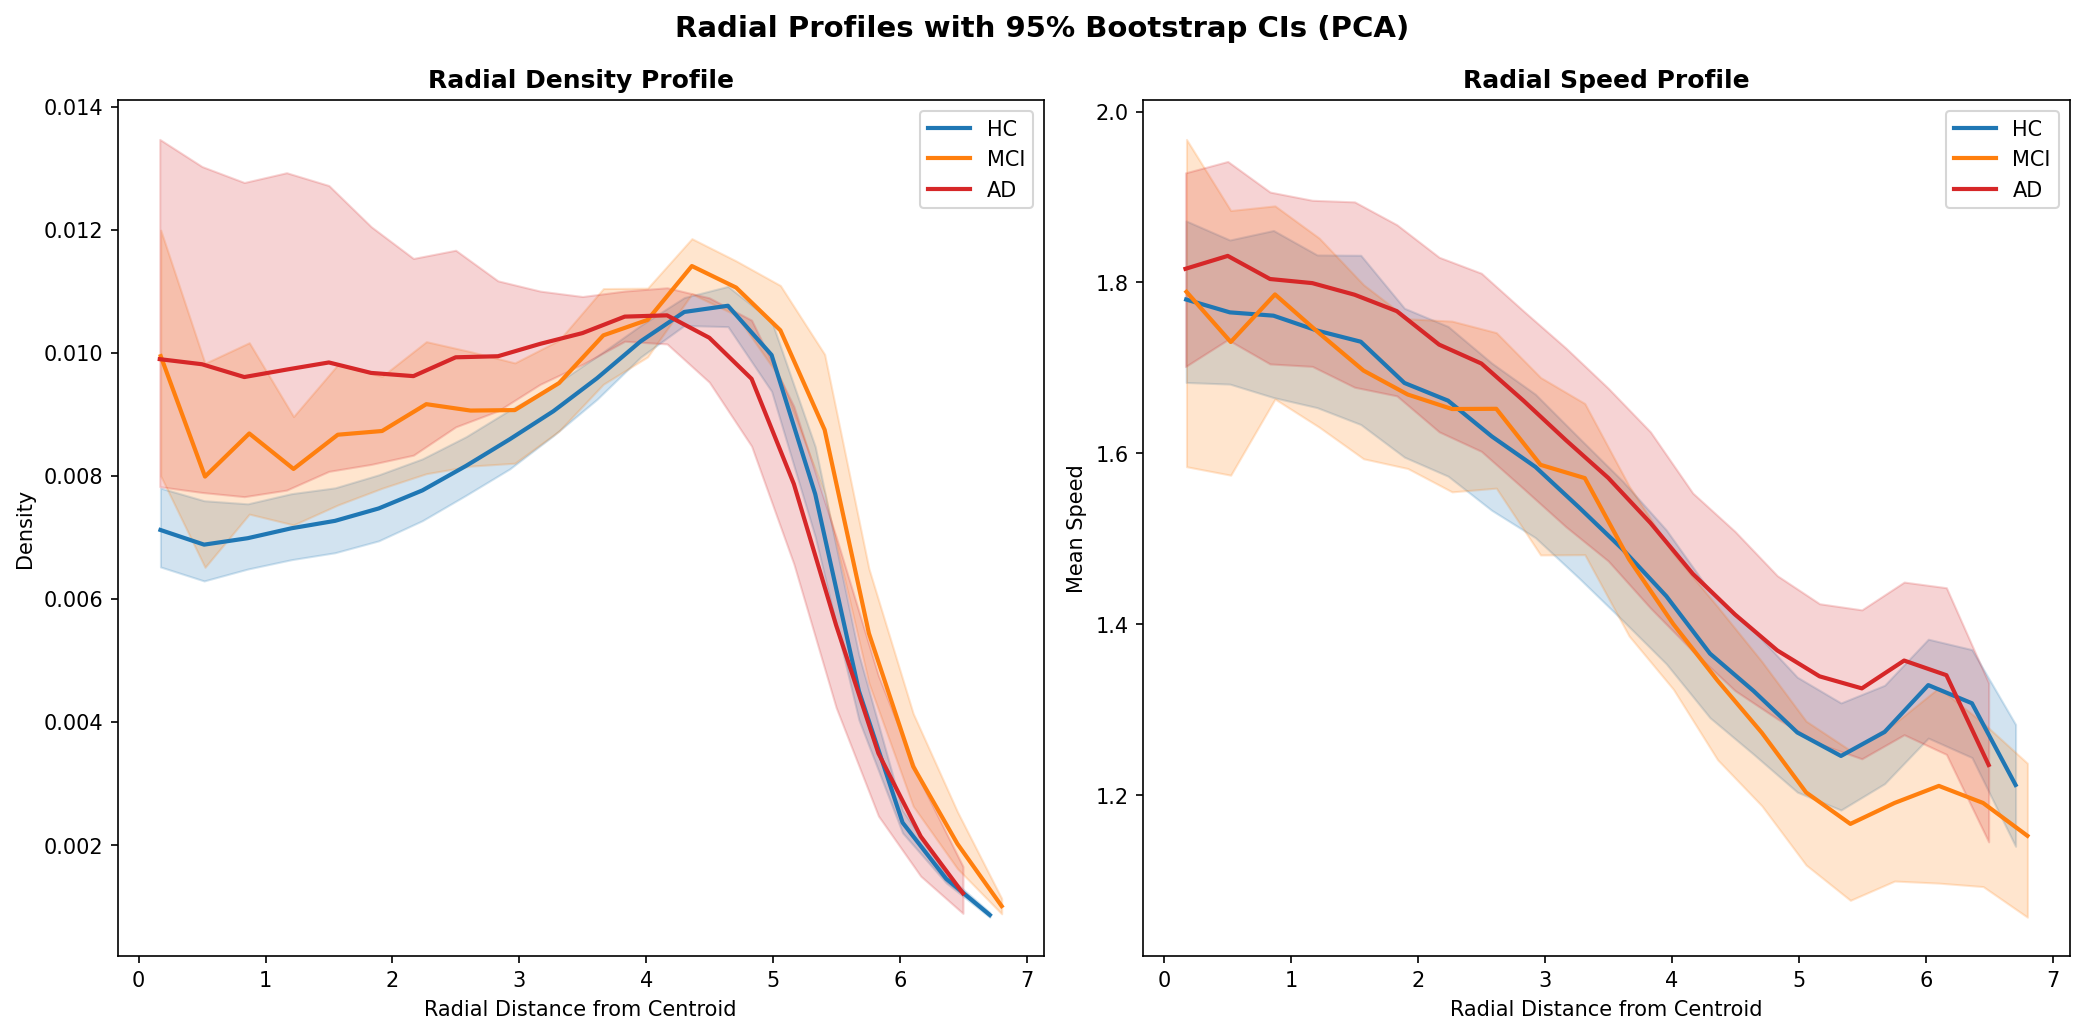
\includegraphics[width=\linewidth]{figures/paper2-wip/radial_profiles_pca.png}
    \caption{Radial profiles of flow metrics. Speed and density are plotted as a function of radial distance from the centroid, showing peripheral vs central dynamics differences.}
    \label{fig:radial_profiles}
\end{figure}

\subsection{Dwell Time Fields}

\figref{fig:dwell_fields} shows spatial distribution of dwell times (low-speed episodes) across the latent space.

\begin{figure}[H]
    \centering
    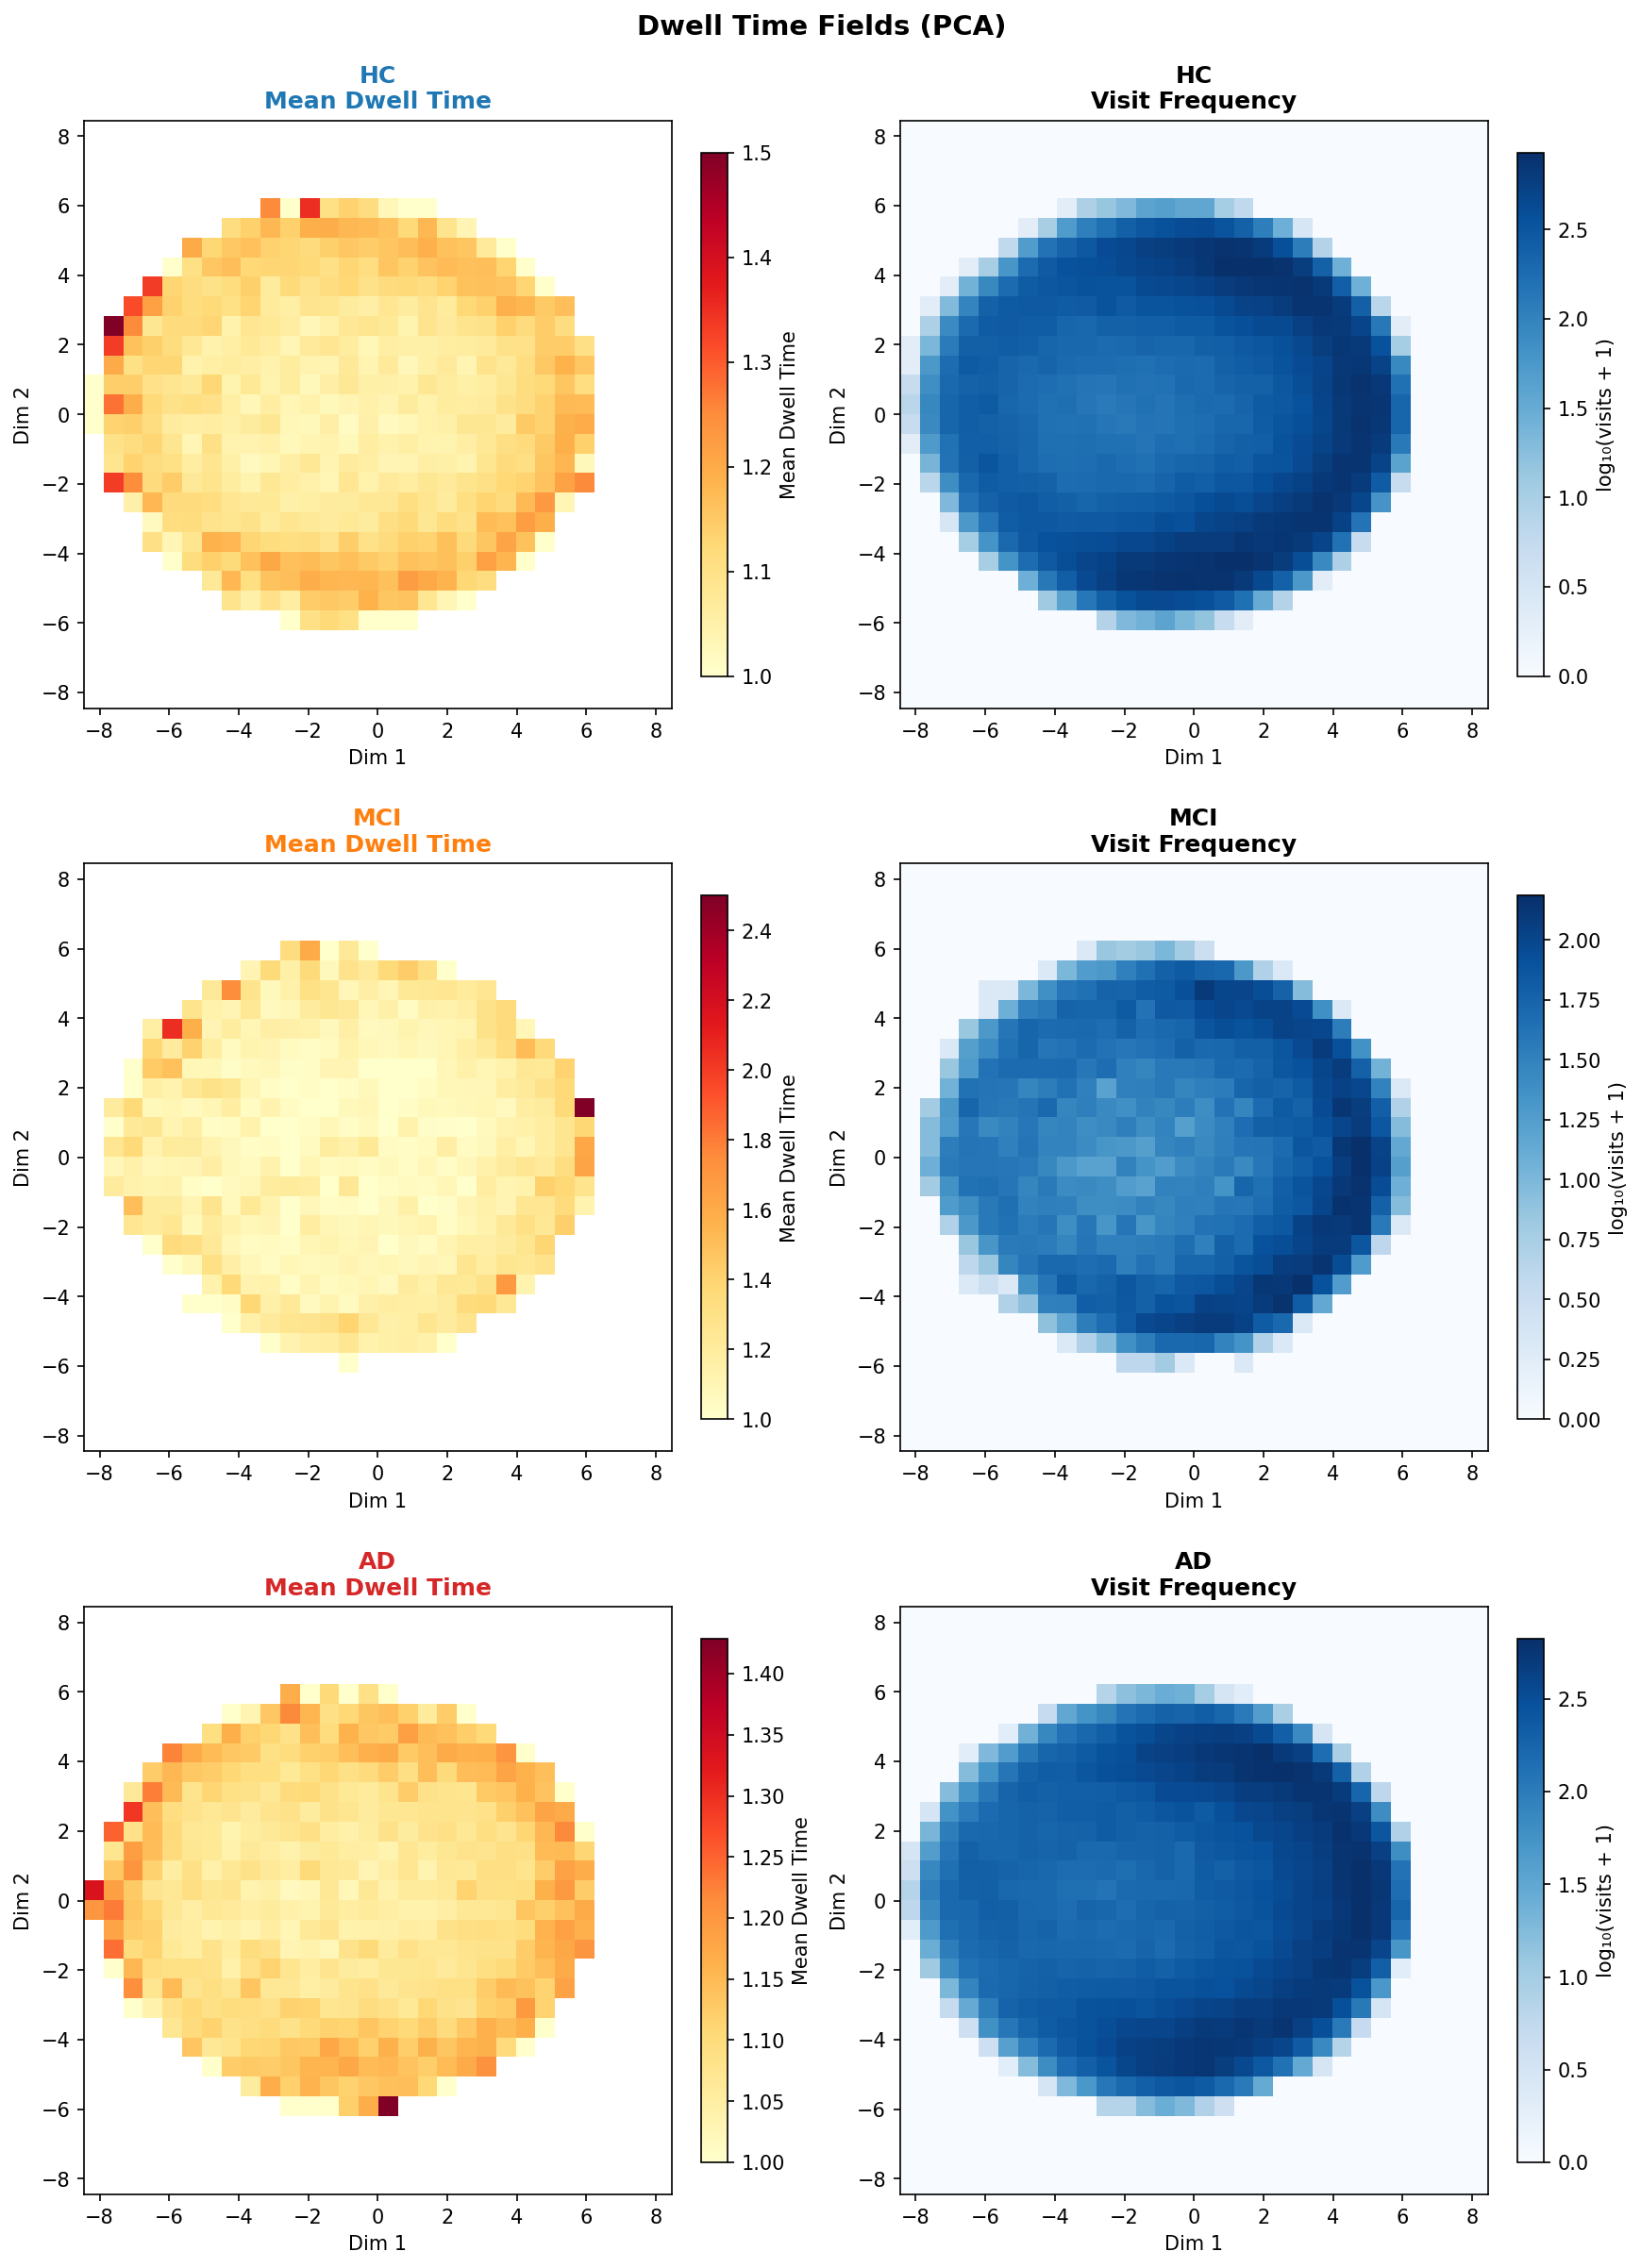
\includegraphics[width=\linewidth]{figures/paper2-wip/dwell_time_fields_pca.png}
    \caption{Dwell time field maps showing where trajectories slow down. Warmer colors indicate longer dwelling; differences reveal where groups pause/linger differently.}
    \label{fig:dwell_fields}
\end{figure}

\subsection{Curvature Analysis}

\figref{fig:curvature} presents trajectory curvature analysis.

\begin{figure}[H]
    \centering
    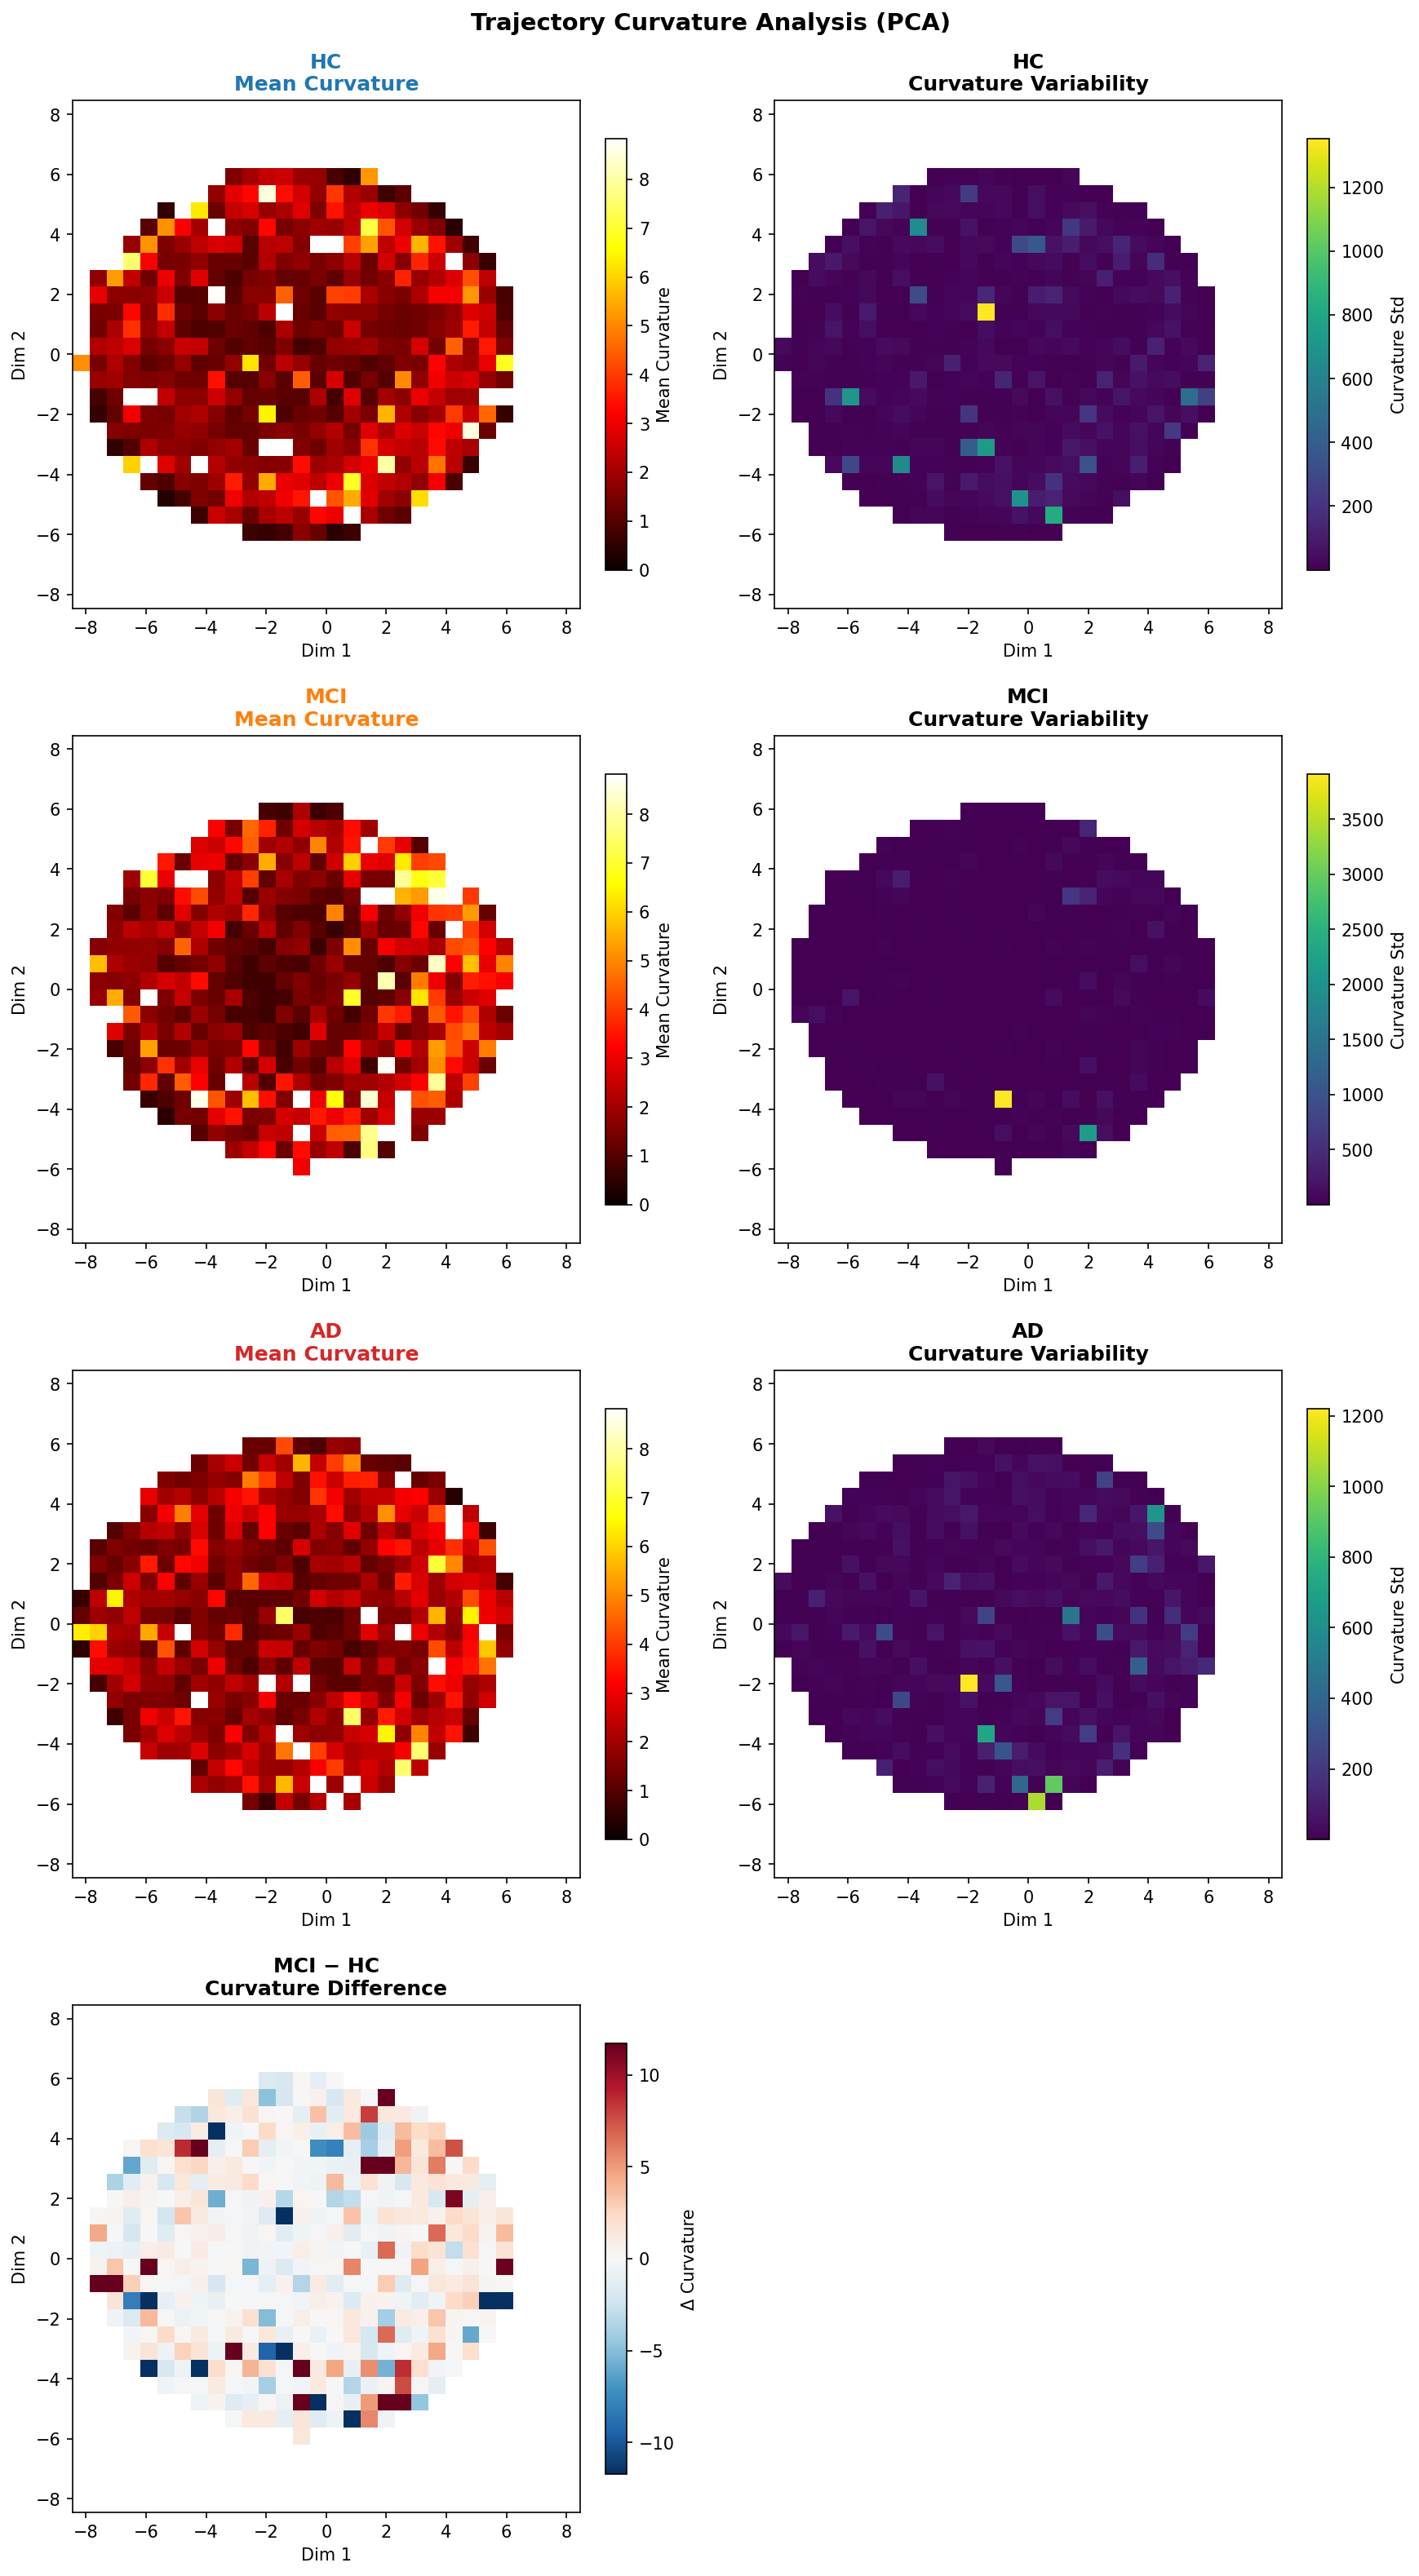
\includegraphics[width=\linewidth]{figures/paper2-wip/curvature_analysis_pca.png}
    \caption{Curvature analysis of latent trajectories. Higher curvature indicates more tortuous, winding paths.}
    \label{fig:curvature}
\end{figure}

\subsection{Streamline Bundles}

\figref{fig:streamlines} visualizes streamline bundles---representative trajectory paths through the flow field.

\begin{figure}[H]
    \centering
    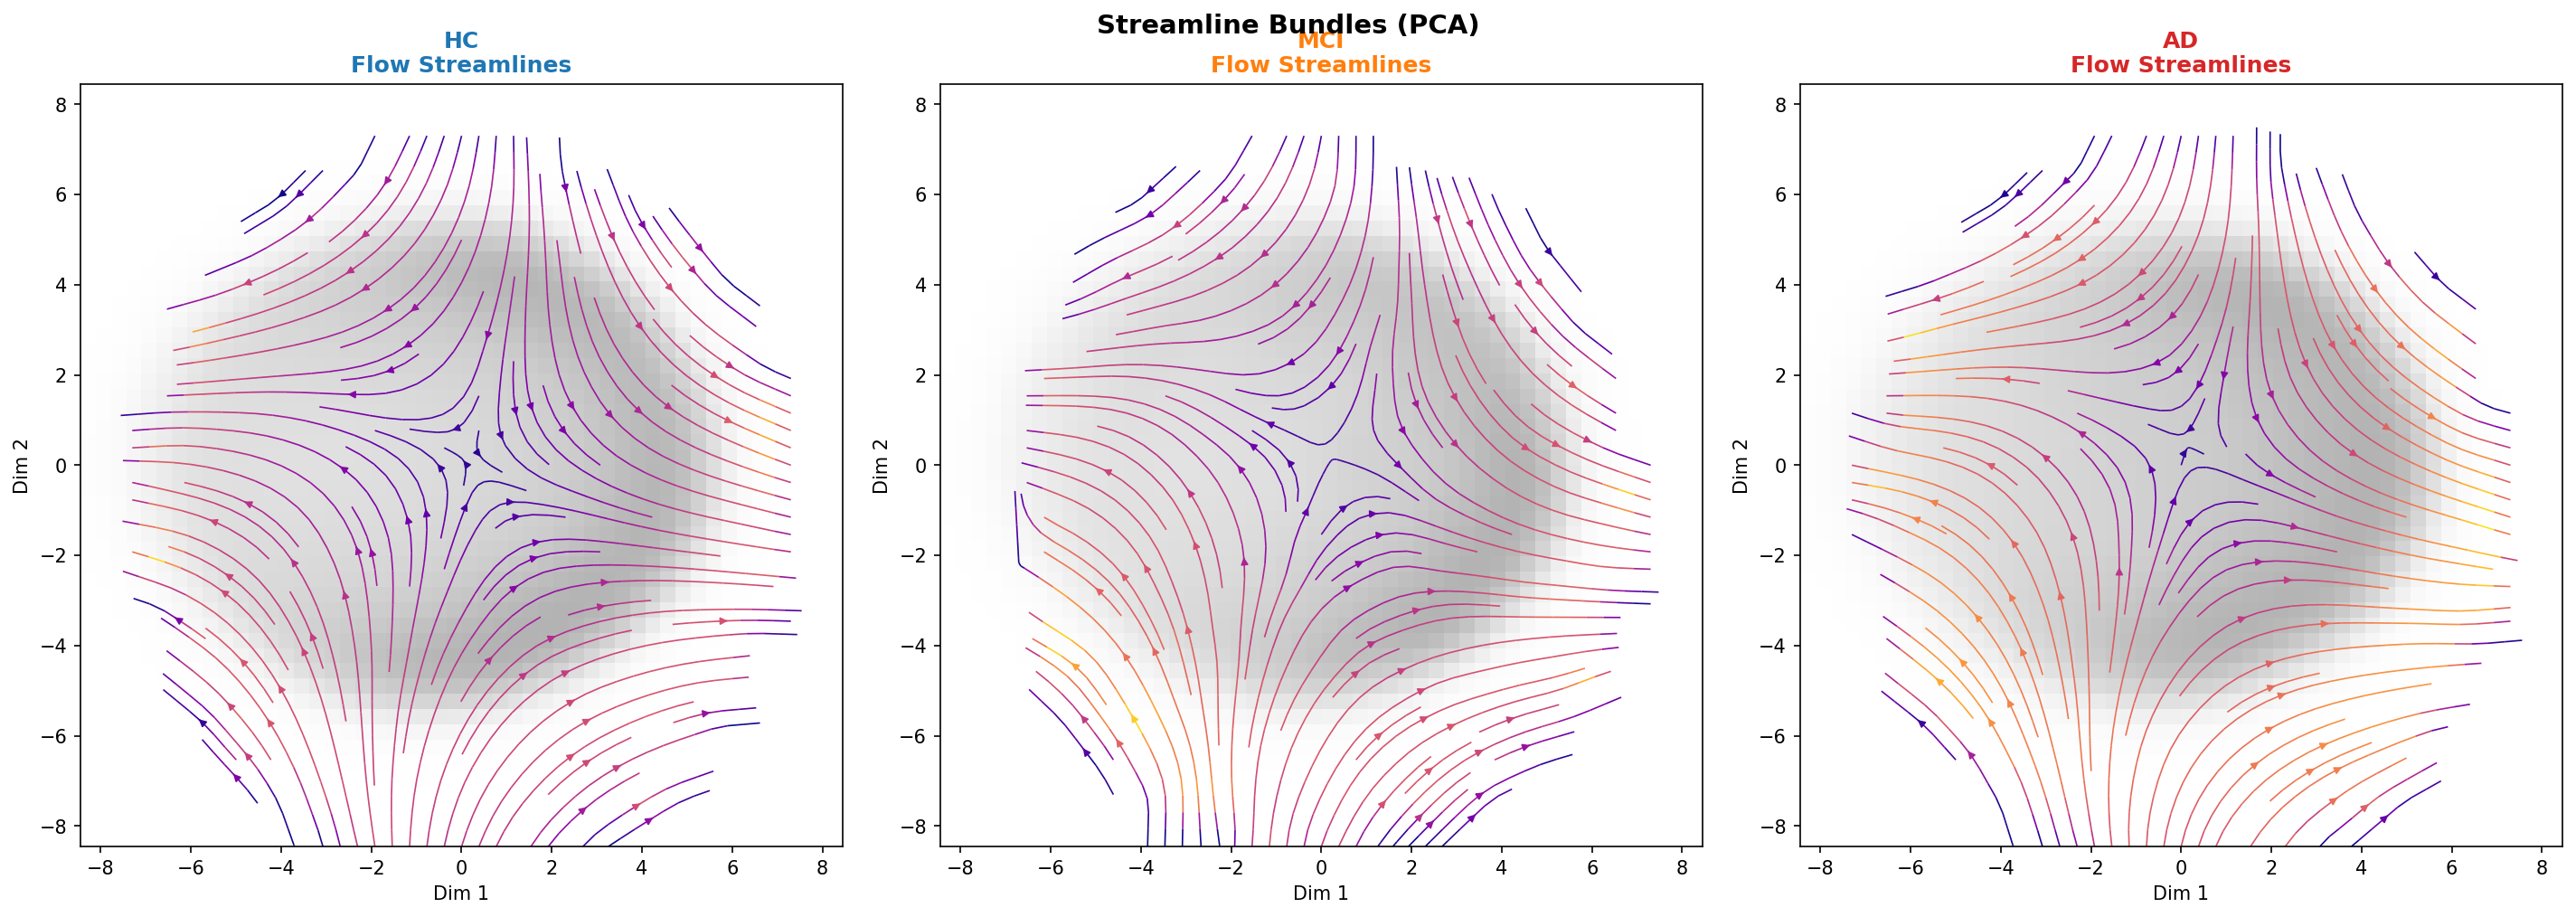
\includegraphics[width=\linewidth]{figures/paper2-wip/streamline_bundles_pca.png}
    \caption{Streamline bundles showing characteristic trajectory paths for each group. Line color indicates local speed; bundles reveal preferred routes through latent space.}
    \label{fig:streamlines}
\end{figure}

\subsection{Directional Entropy and Temporal Heterogeneity}

\figref{fig:directional_entropy} and \figref{fig:temporal_heterogeneity} provide additional dynamical characterization.

\begin{figure}[H]
    \centering
    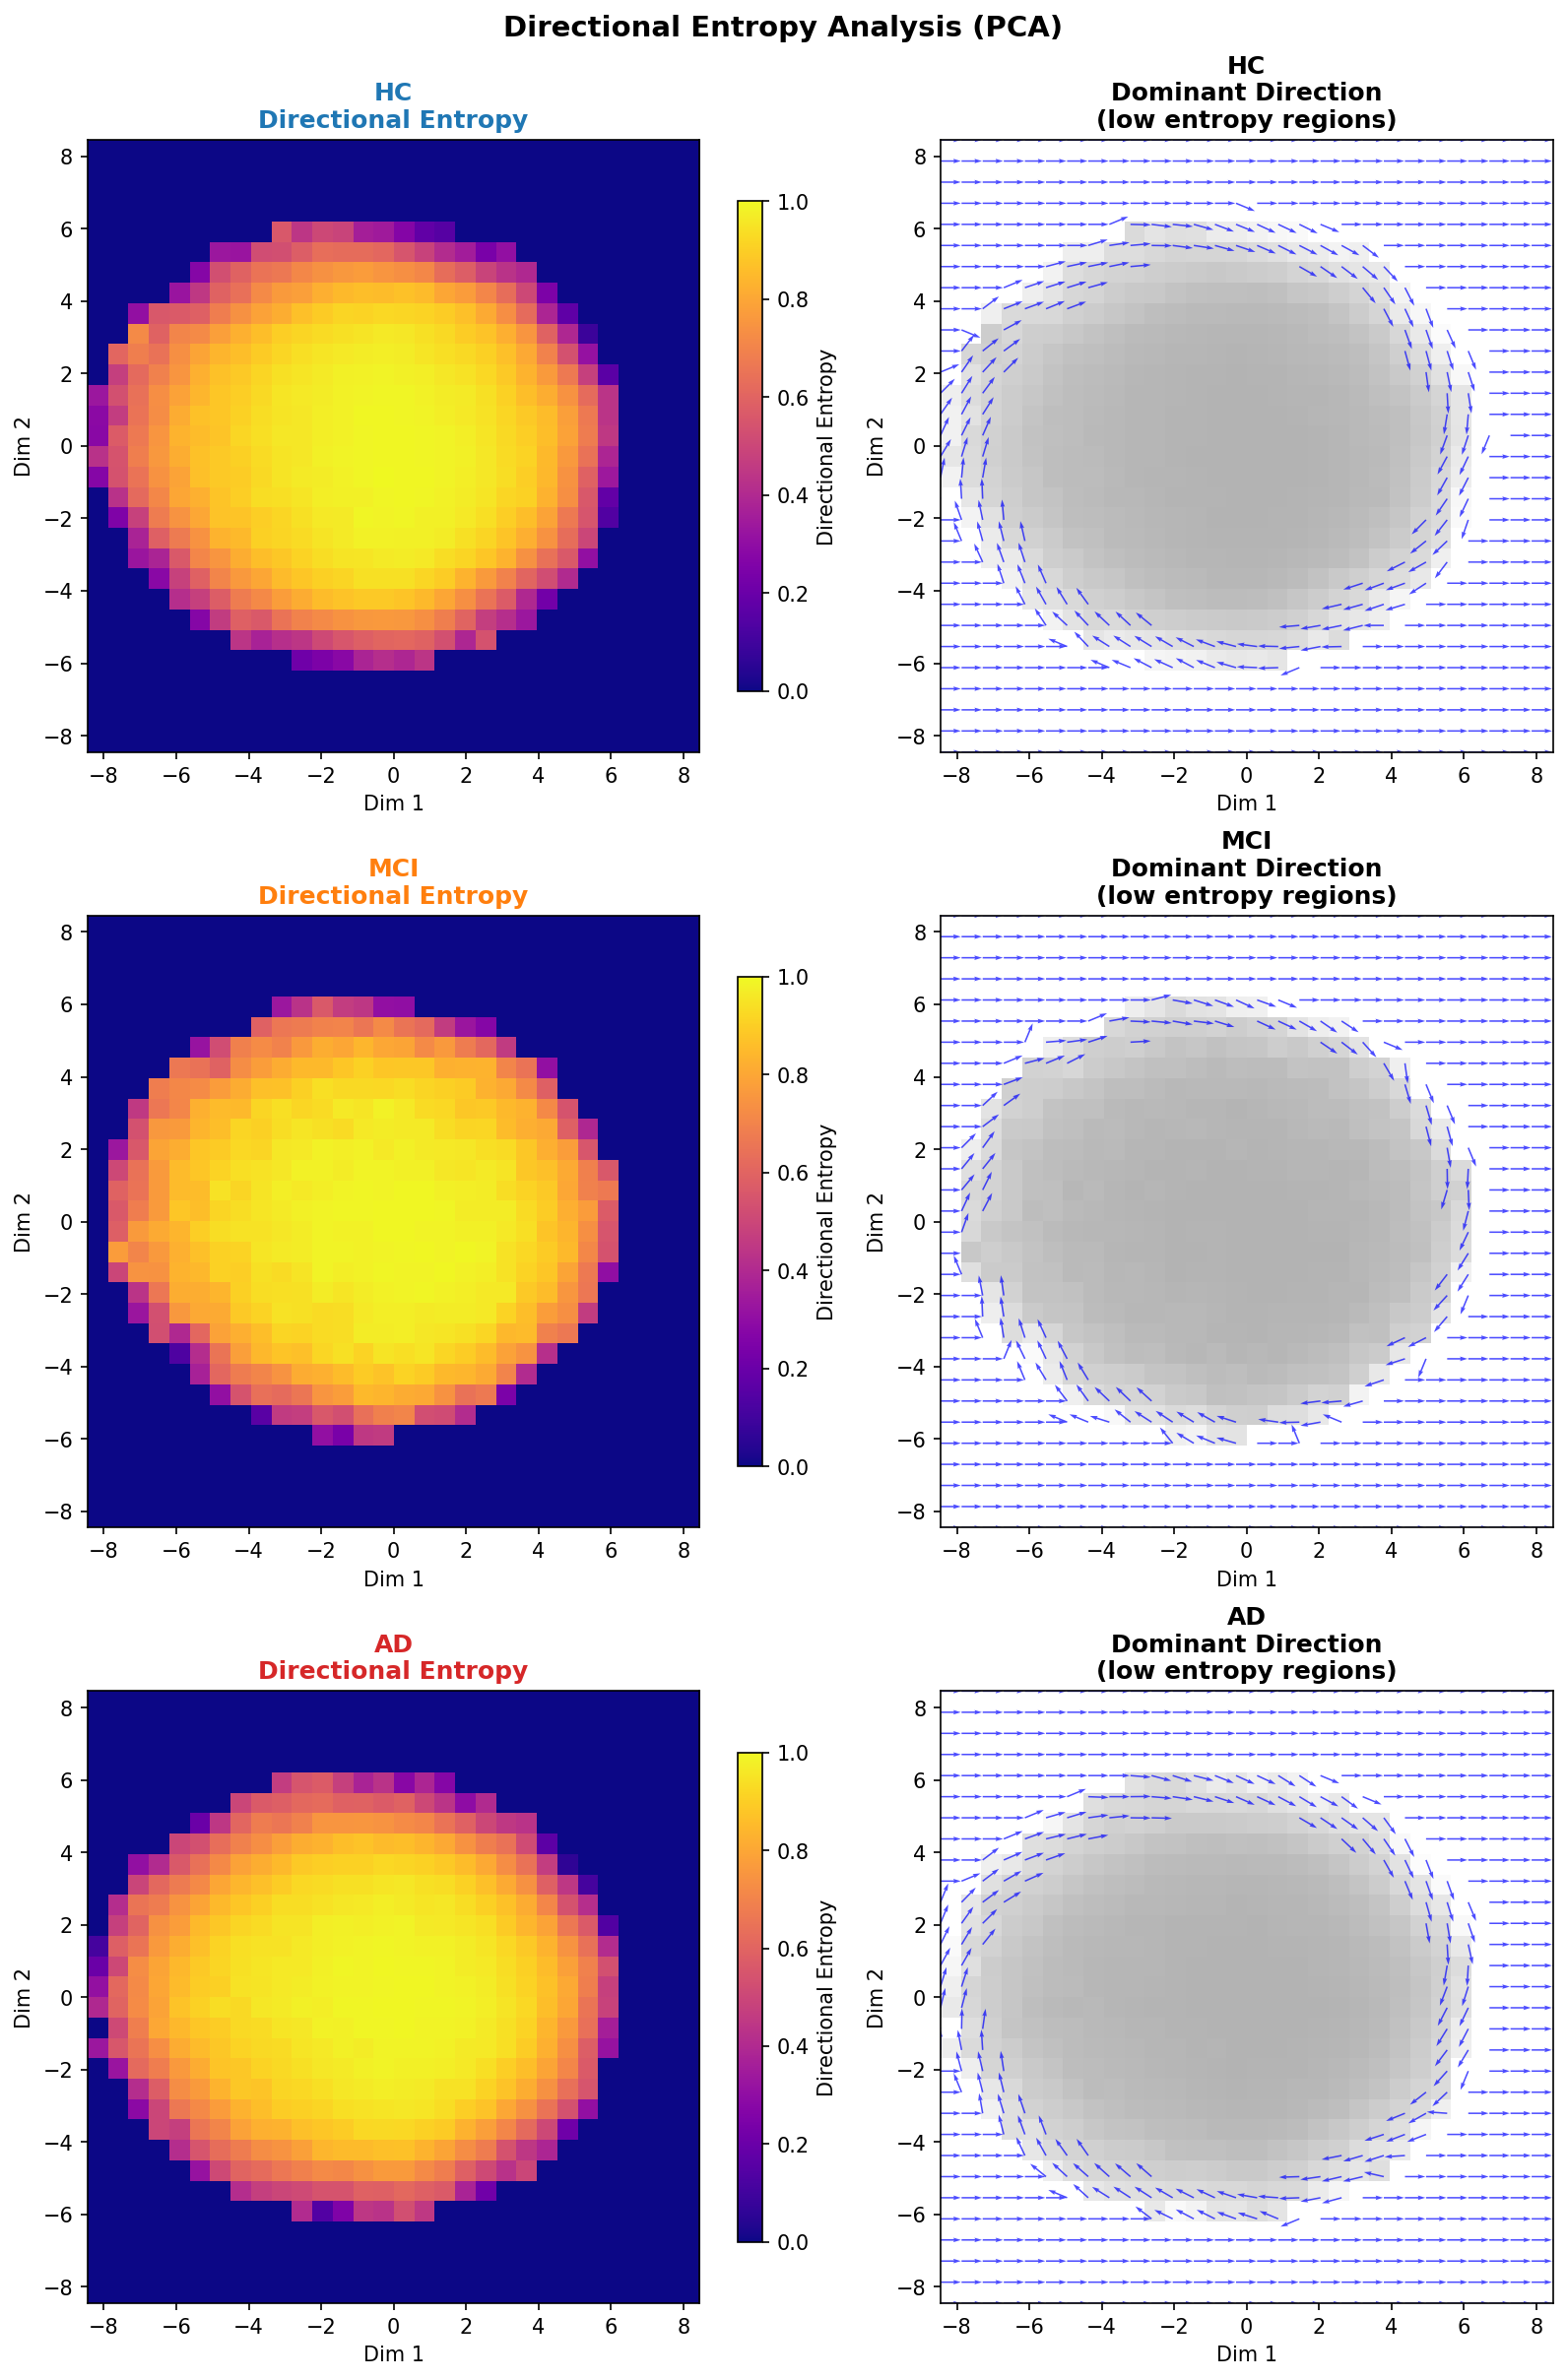
\includegraphics[width=\linewidth]{figures/paper2-wip/directional_entropy_pca.png}
    \caption{Directional entropy maps showing regions of high vs low predictability in flow direction.}
    \label{fig:directional_entropy}
\end{figure}

\begin{figure}[H]
    \centering
    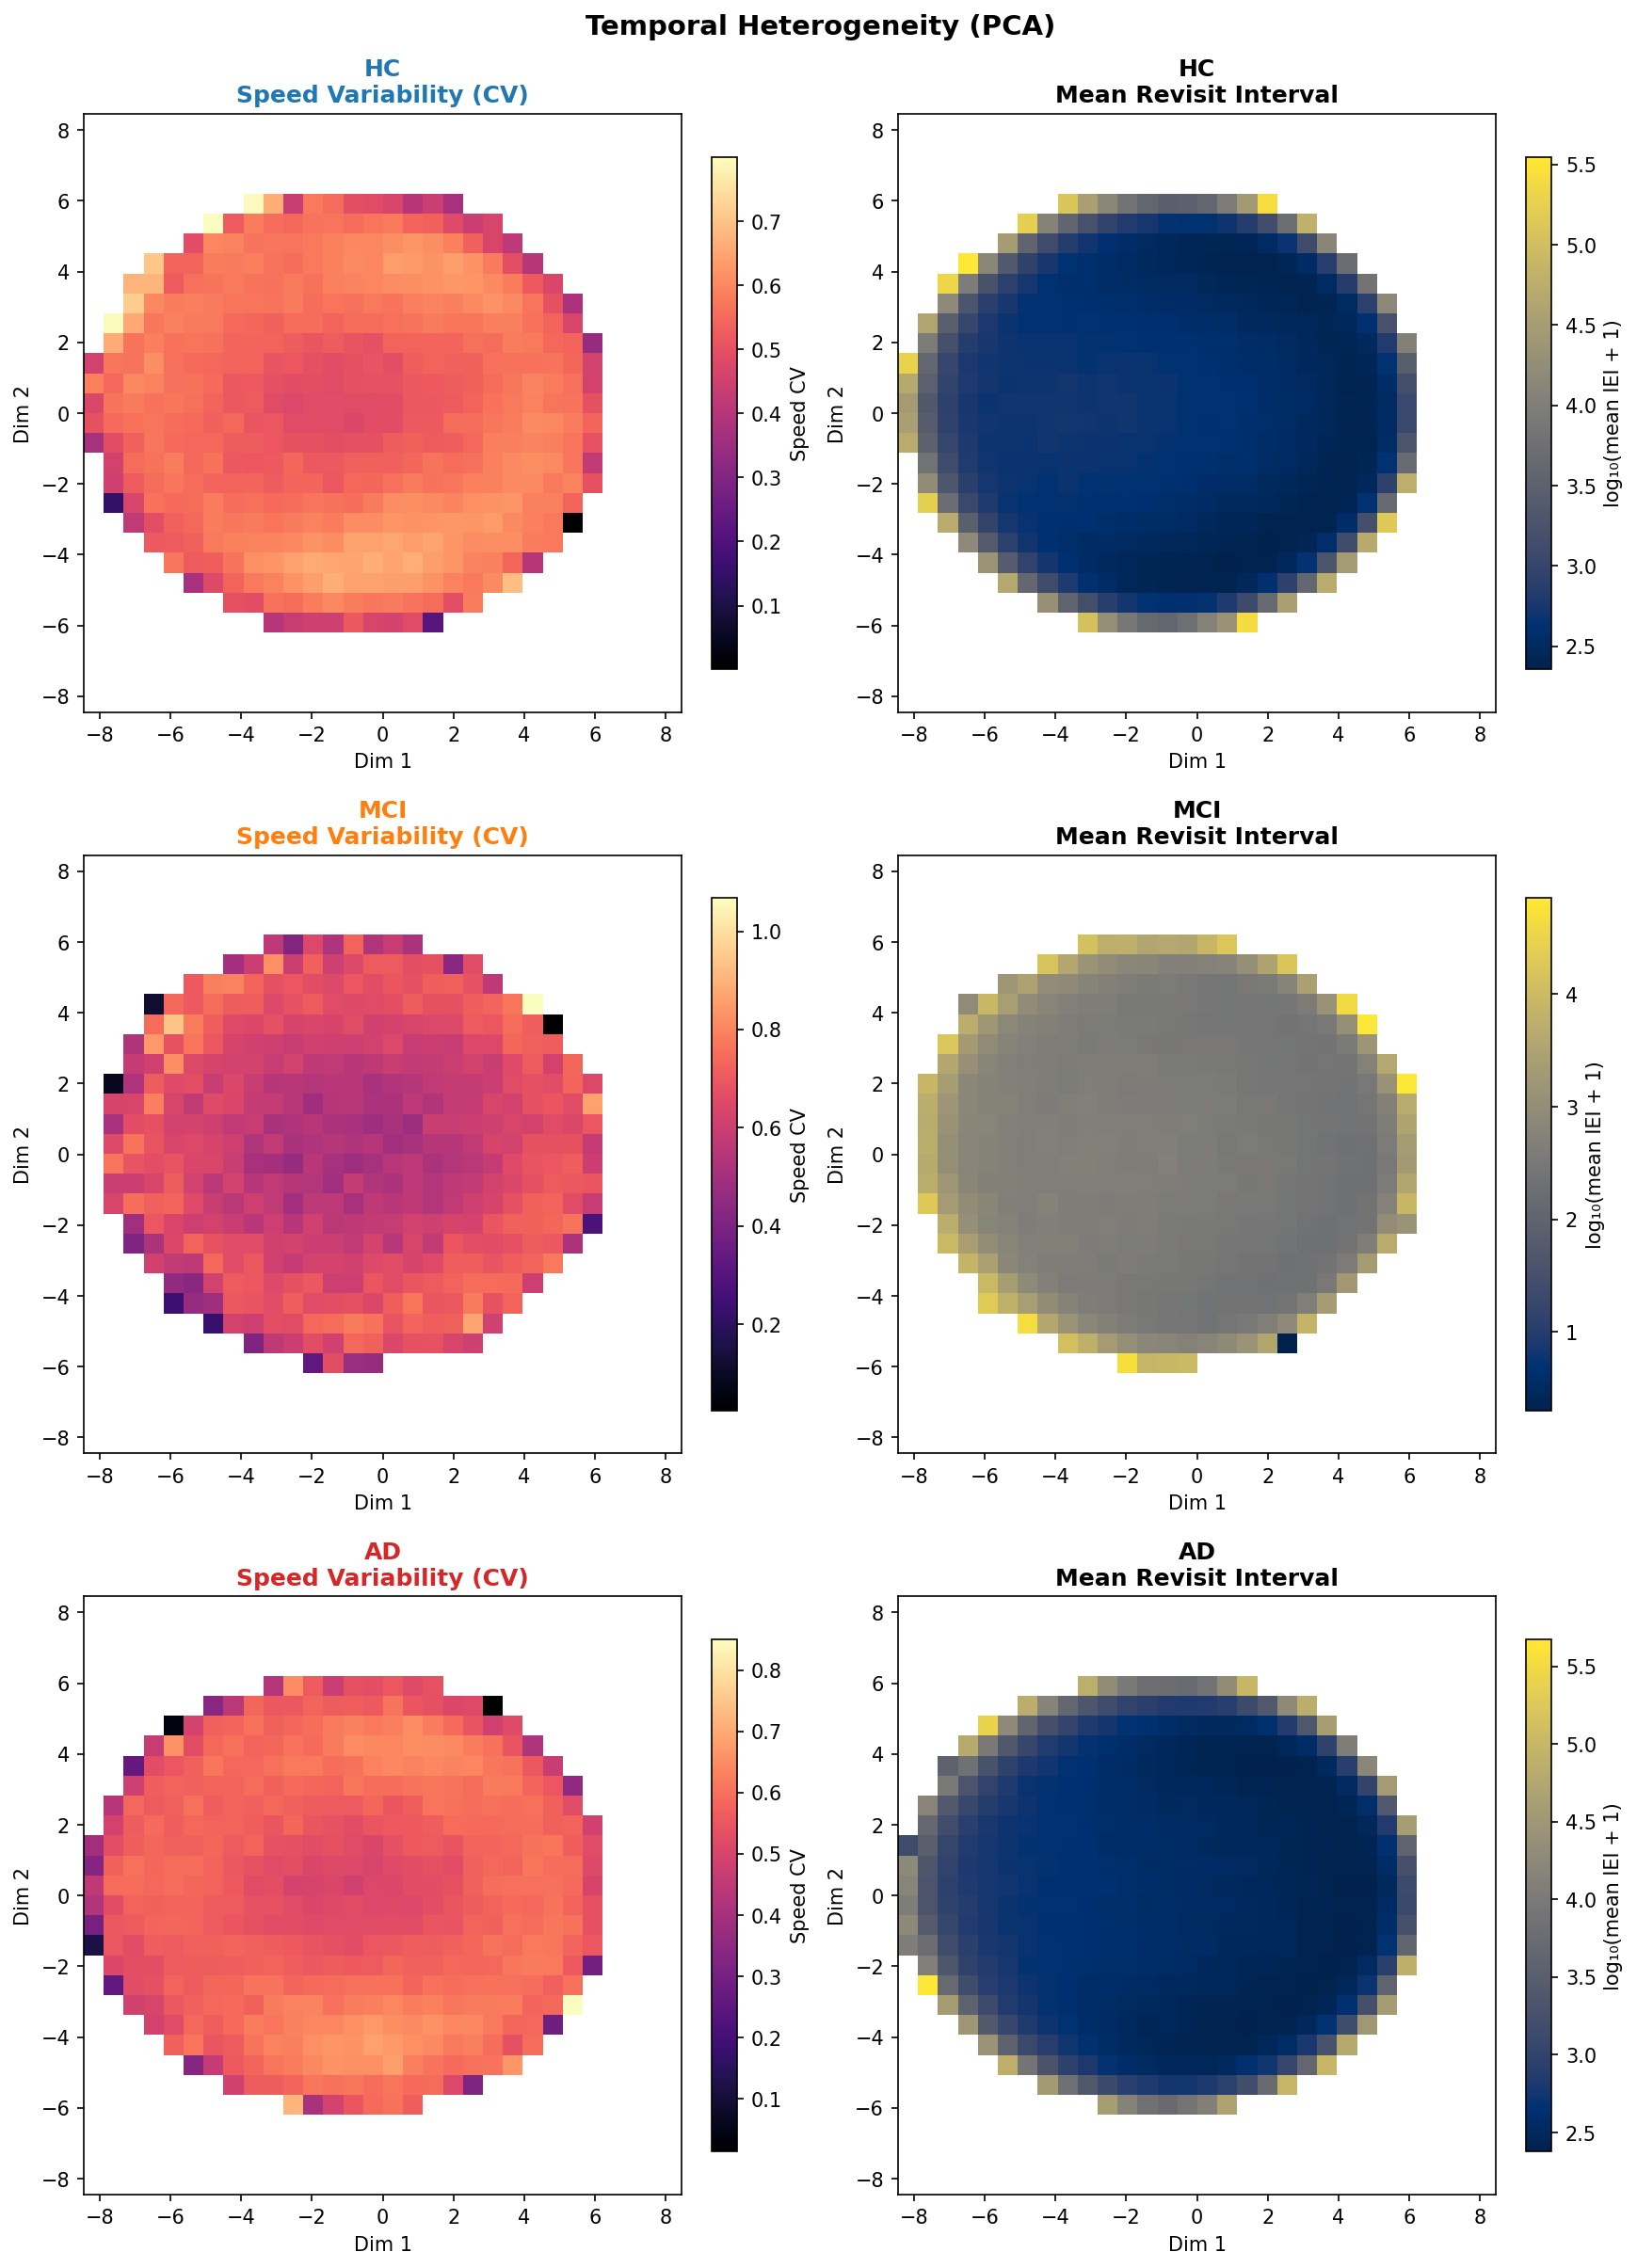
\includegraphics[width=\linewidth]{figures/paper2-wip/temporal_heterogeneity_pca.png}
    \caption{Temporal heterogeneity analysis showing how flow structure changes over time.}
    \label{fig:temporal_heterogeneity}
\end{figure}

\subsection{Cross-Embedding Robustness}

\figref{fig:cross_embedding} examines metric consistency across different embedding methods.

\begin{figure}[H]
    \centering
    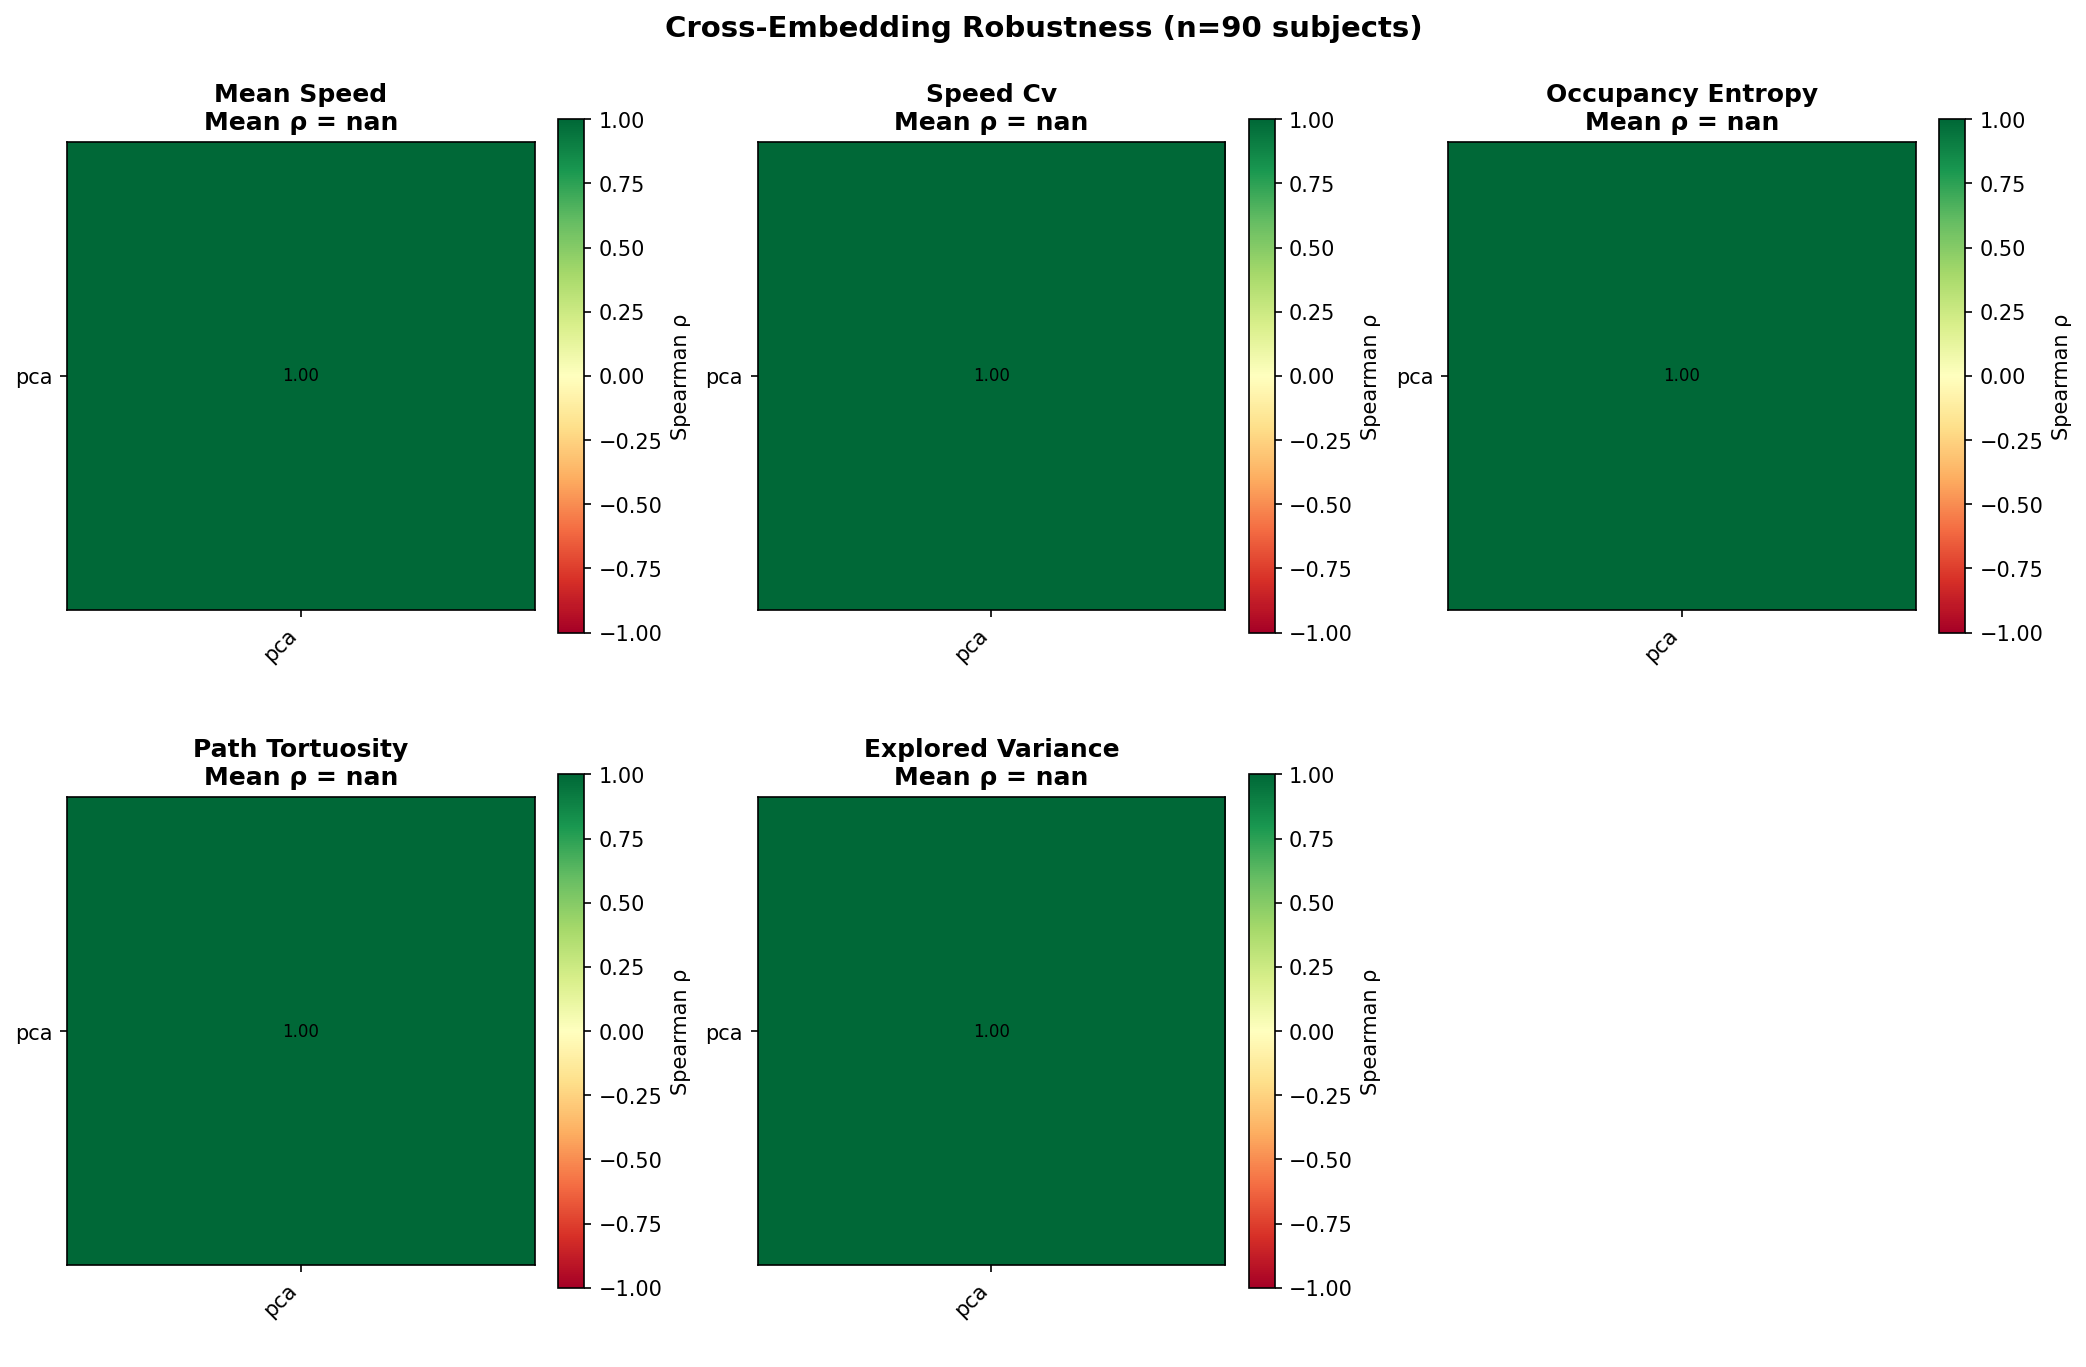
\includegraphics[width=\linewidth]{figures/paper2-wip/cross_embedding_robustness.png}
    \caption{Cross-embedding robustness analysis. Metrics are compared across PCA, t-SNE, and UMAP projections to verify that group differences are not embedding-dependent artifacts.}
    \label{fig:cross_embedding}
\end{figure}

% =========================
\section{Results: MCI Subtype Analysis}
\label{sec:subtypes}
% =========================

We stratified the MCI cohort ($n = 82$) by two clinical dimensions:
\begin{enumerate}
    \item \textbf{MMSE Severity}: Low ($<24$), Mid ($24$--$26$), High ($>26$)
    \item \textbf{Functional Impairment}: Low (mild), Mid (moderate), High (severe)
\end{enumerate}

\subsection{MMSE Severity Stratification}

\subsubsection{Bootstrap Metrics}

\figref{fig:mmse_bootstrap} shows flow metric distributions stratified by MMSE severity.

\begin{figure}[H]
    \centering
    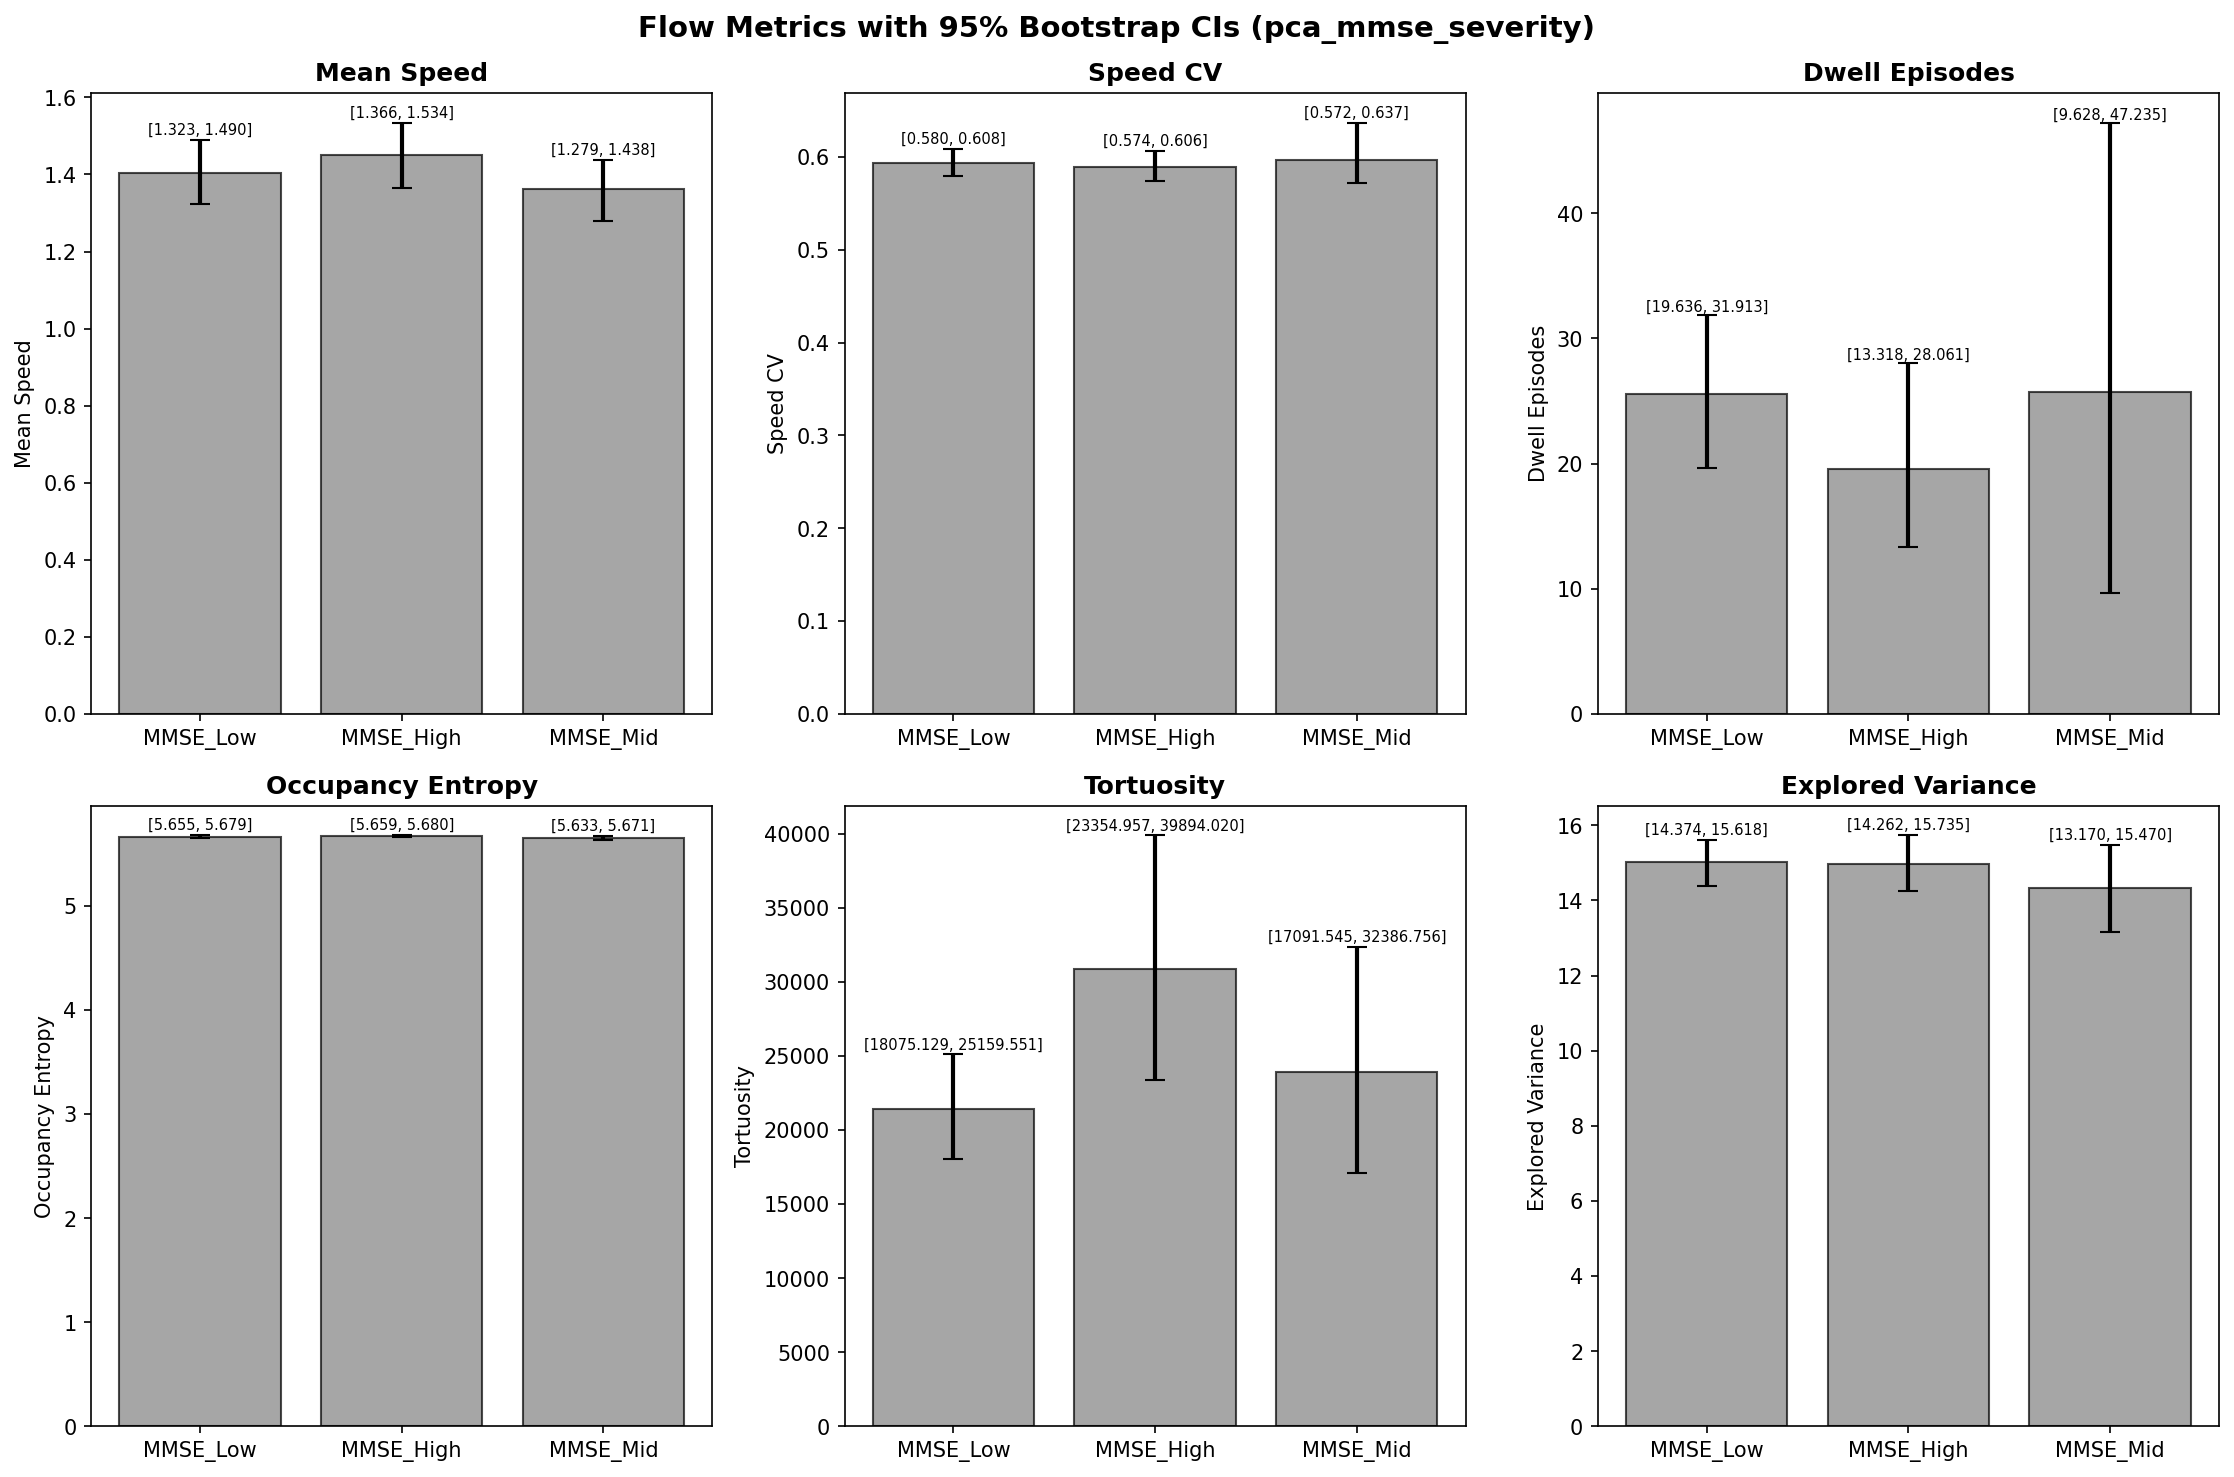
\includegraphics[width=\linewidth]{figures/paper2-wip/bootstrap_metrics_pca_mmse_severity.png}
    \caption{Bootstrap distributions of flow metrics stratified by MMSE severity (Low, Mid, High). Higher MMSE indicates better cognitive function.}
    \label{fig:mmse_bootstrap}
\end{figure}

\textbf{Key findings by MMSE severity}:
\begin{itemize}
    \item \textbf{Path Tortuosity}: MMSE Low vs High shows $d = -0.58$ [-1.11, -0.04] --- lower cognitive function associated with \emph{lower} tortuosity (less complex paths)
    \item \textbf{Mean Speed}: MMSE High shows trend toward faster dynamics ($d = 0.46$ [-0.14, 1.03] for High vs Mid)
    \item Other metrics show overlapping confidence intervals
\end{itemize}

\subsubsection{Flow Fields by MMSE}

\figref{fig:mmse_flow_fields} and \figref{fig:mmse_flow_diff} show flow field structure by MMSE group.

\begin{figure}[H]
    \centering
    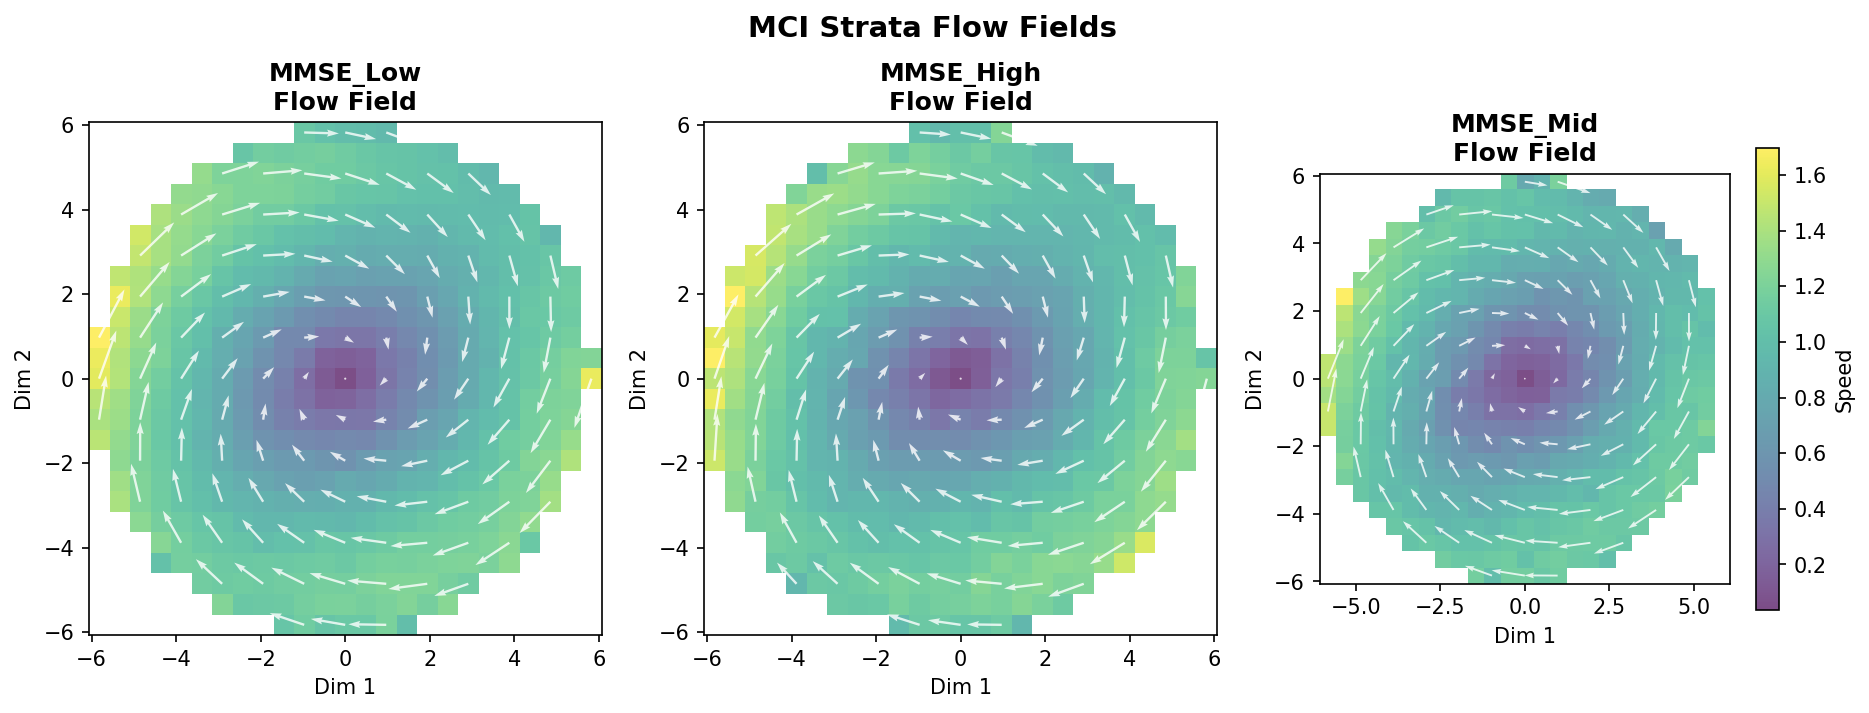
\includegraphics[width=\linewidth]{figures/paper2-wip/flow_fields_pca_mmse_severity.png}
    \caption{Flow fields stratified by MMSE severity group.}
    \label{fig:mmse_flow_fields}
\end{figure}

\begin{figure}[H]
    \centering
    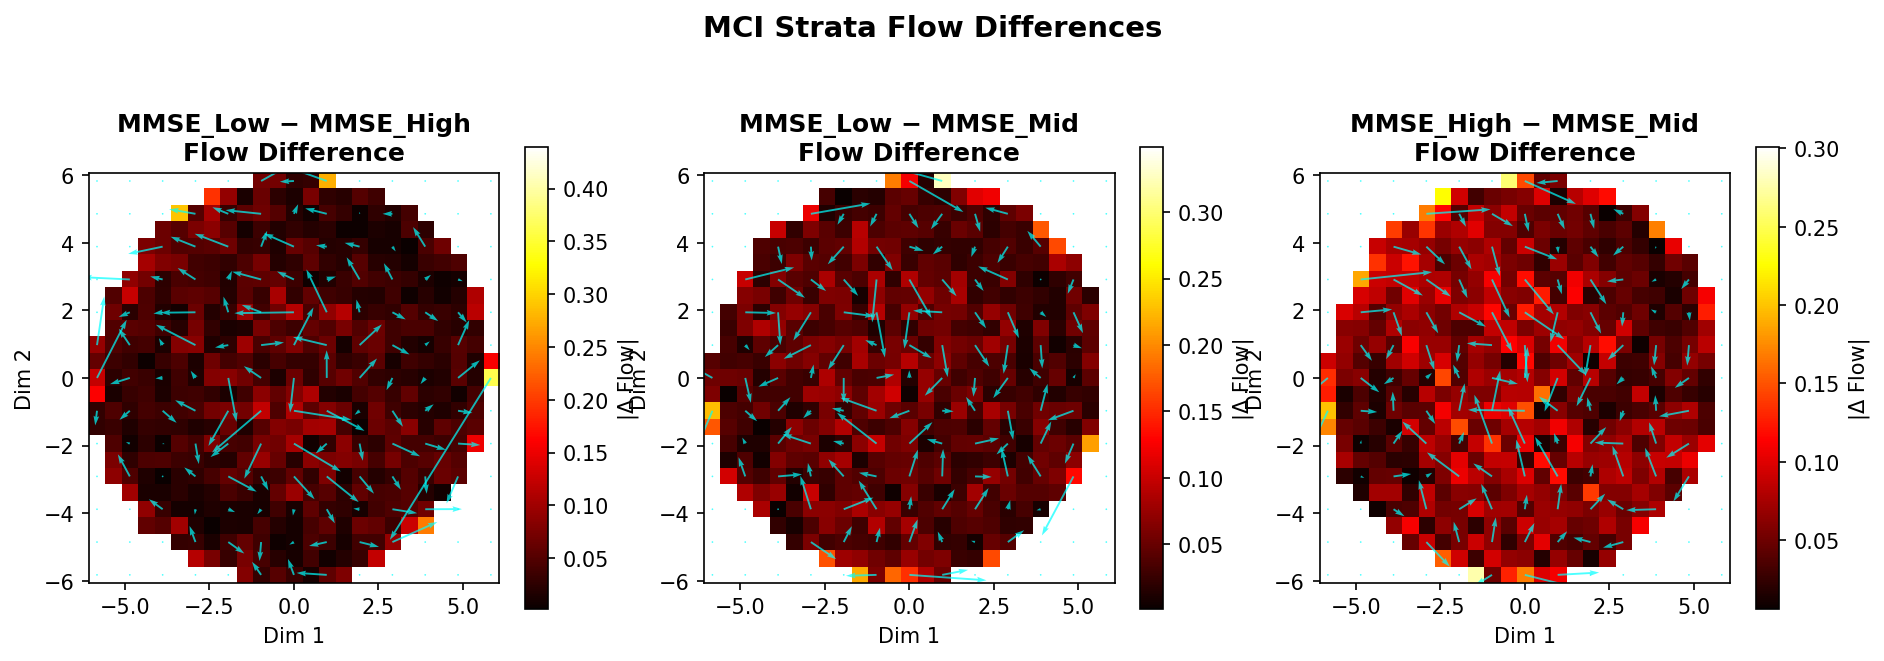
\includegraphics[width=\linewidth]{figures/paper2-wip/flow_difference_pca_mmse_severity.png}
    \caption{Flow field differences between MMSE severity groups.}
    \label{fig:mmse_flow_diff}
\end{figure}

\subsubsection{Radial Profiles and Dwell Fields}

\begin{figure}[H]
    \centering
    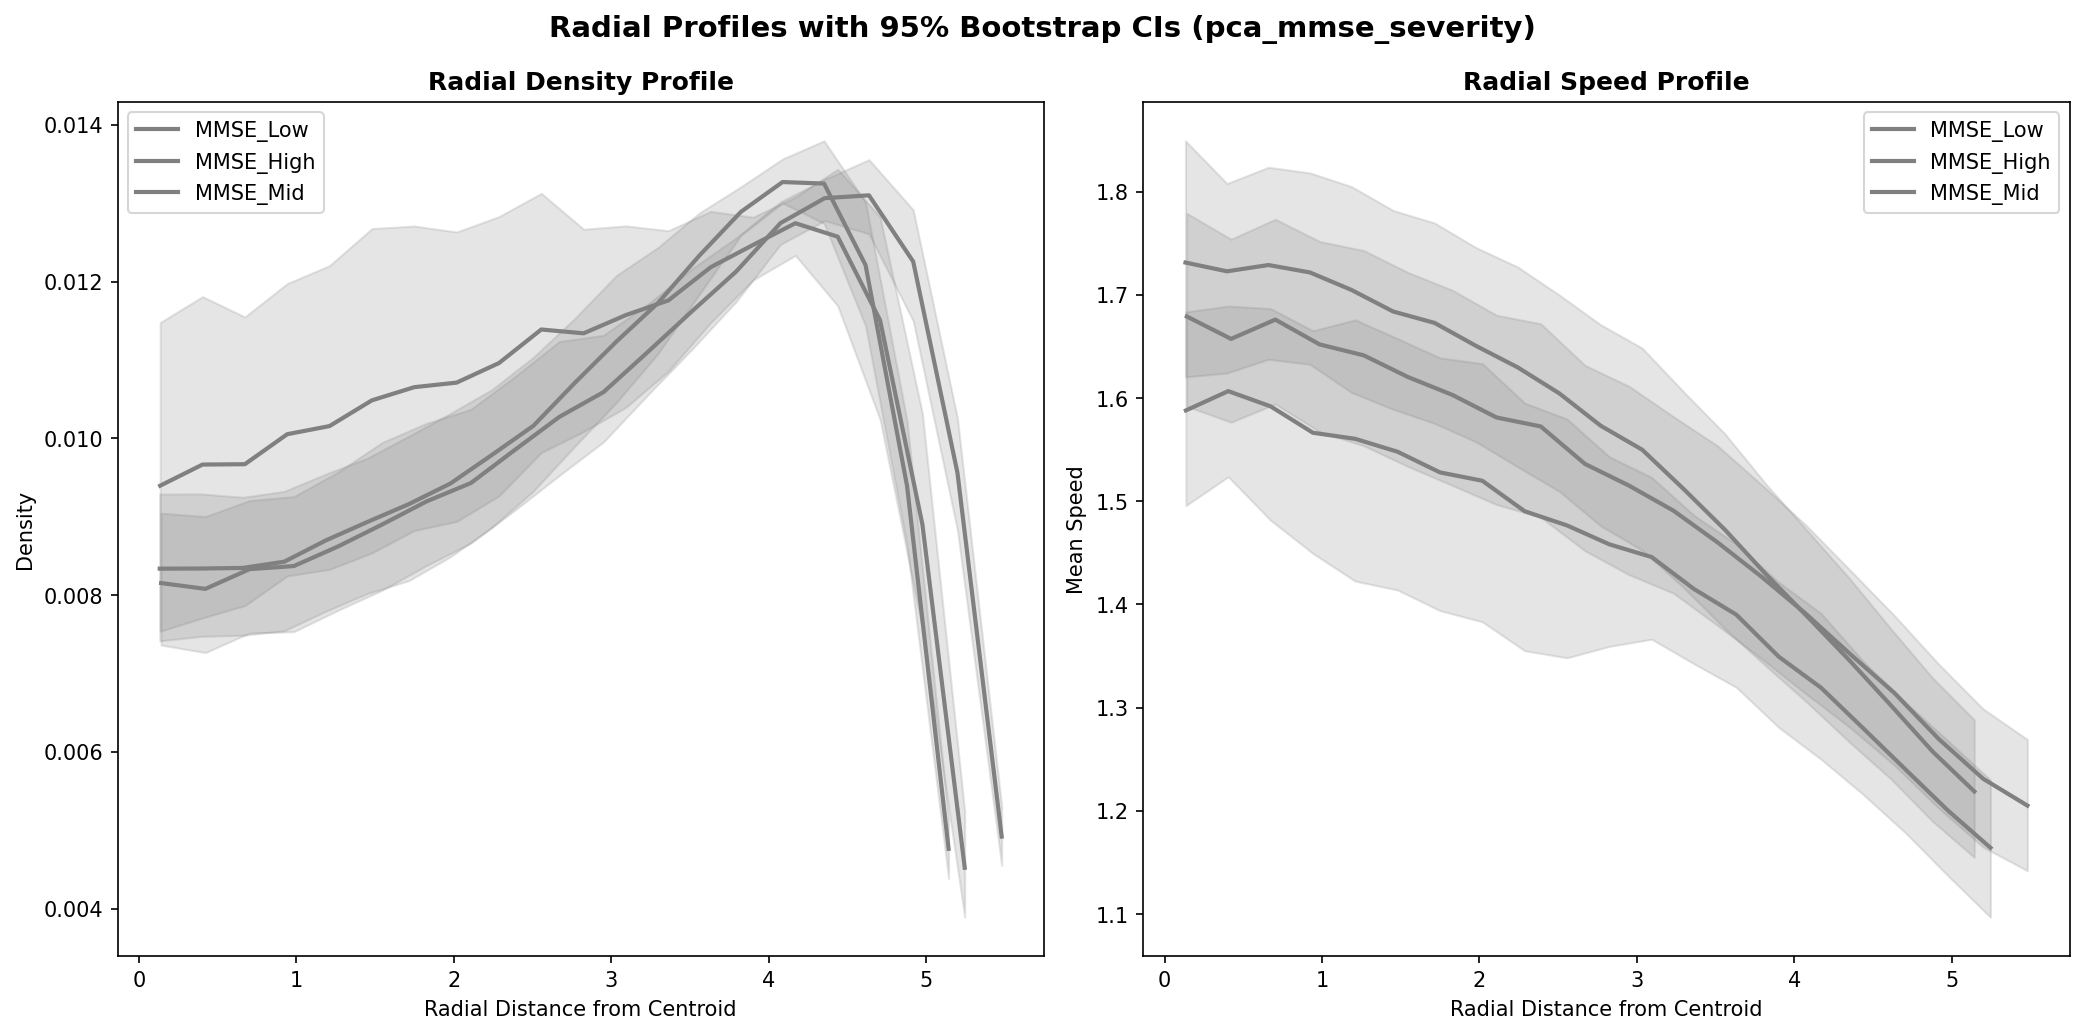
\includegraphics[width=\linewidth]{figures/paper2-wip/radial_profiles_pca_mmse_severity.png}
    \caption{Radial profiles by MMSE severity.}
    \label{fig:mmse_radial}
\end{figure}

\begin{figure}[H]
    \centering
    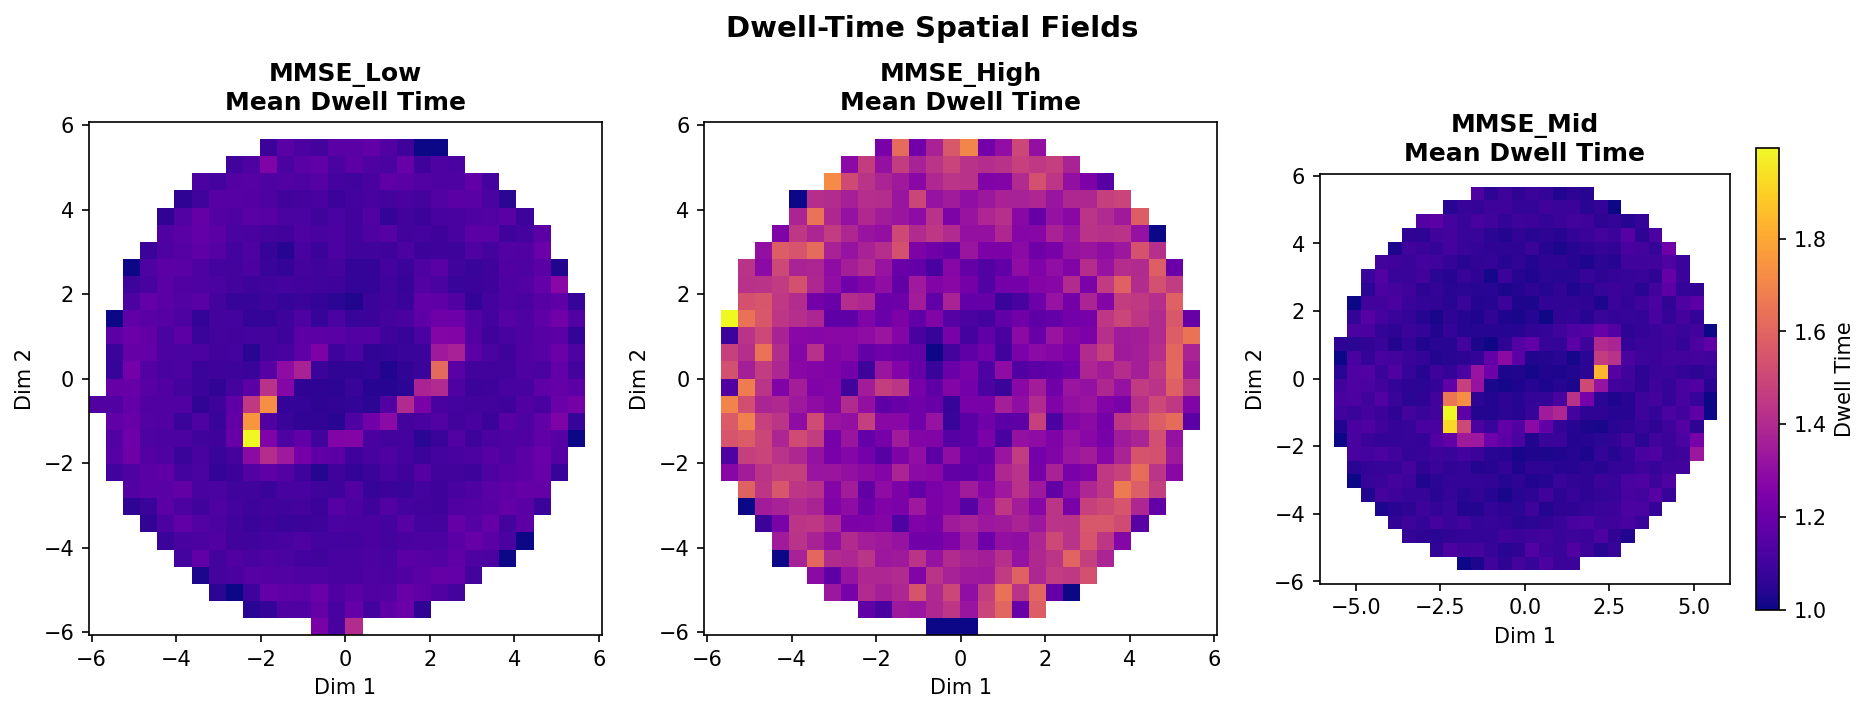
\includegraphics[width=\linewidth]{figures/paper2-wip/dwell_time_fields_pca_mmse_severity.png}
    \caption{Dwell time fields by MMSE severity.}
    \label{fig:mmse_dwell}
\end{figure}

\subsubsection{Density Differences}

\begin{figure}[H]
    \centering
    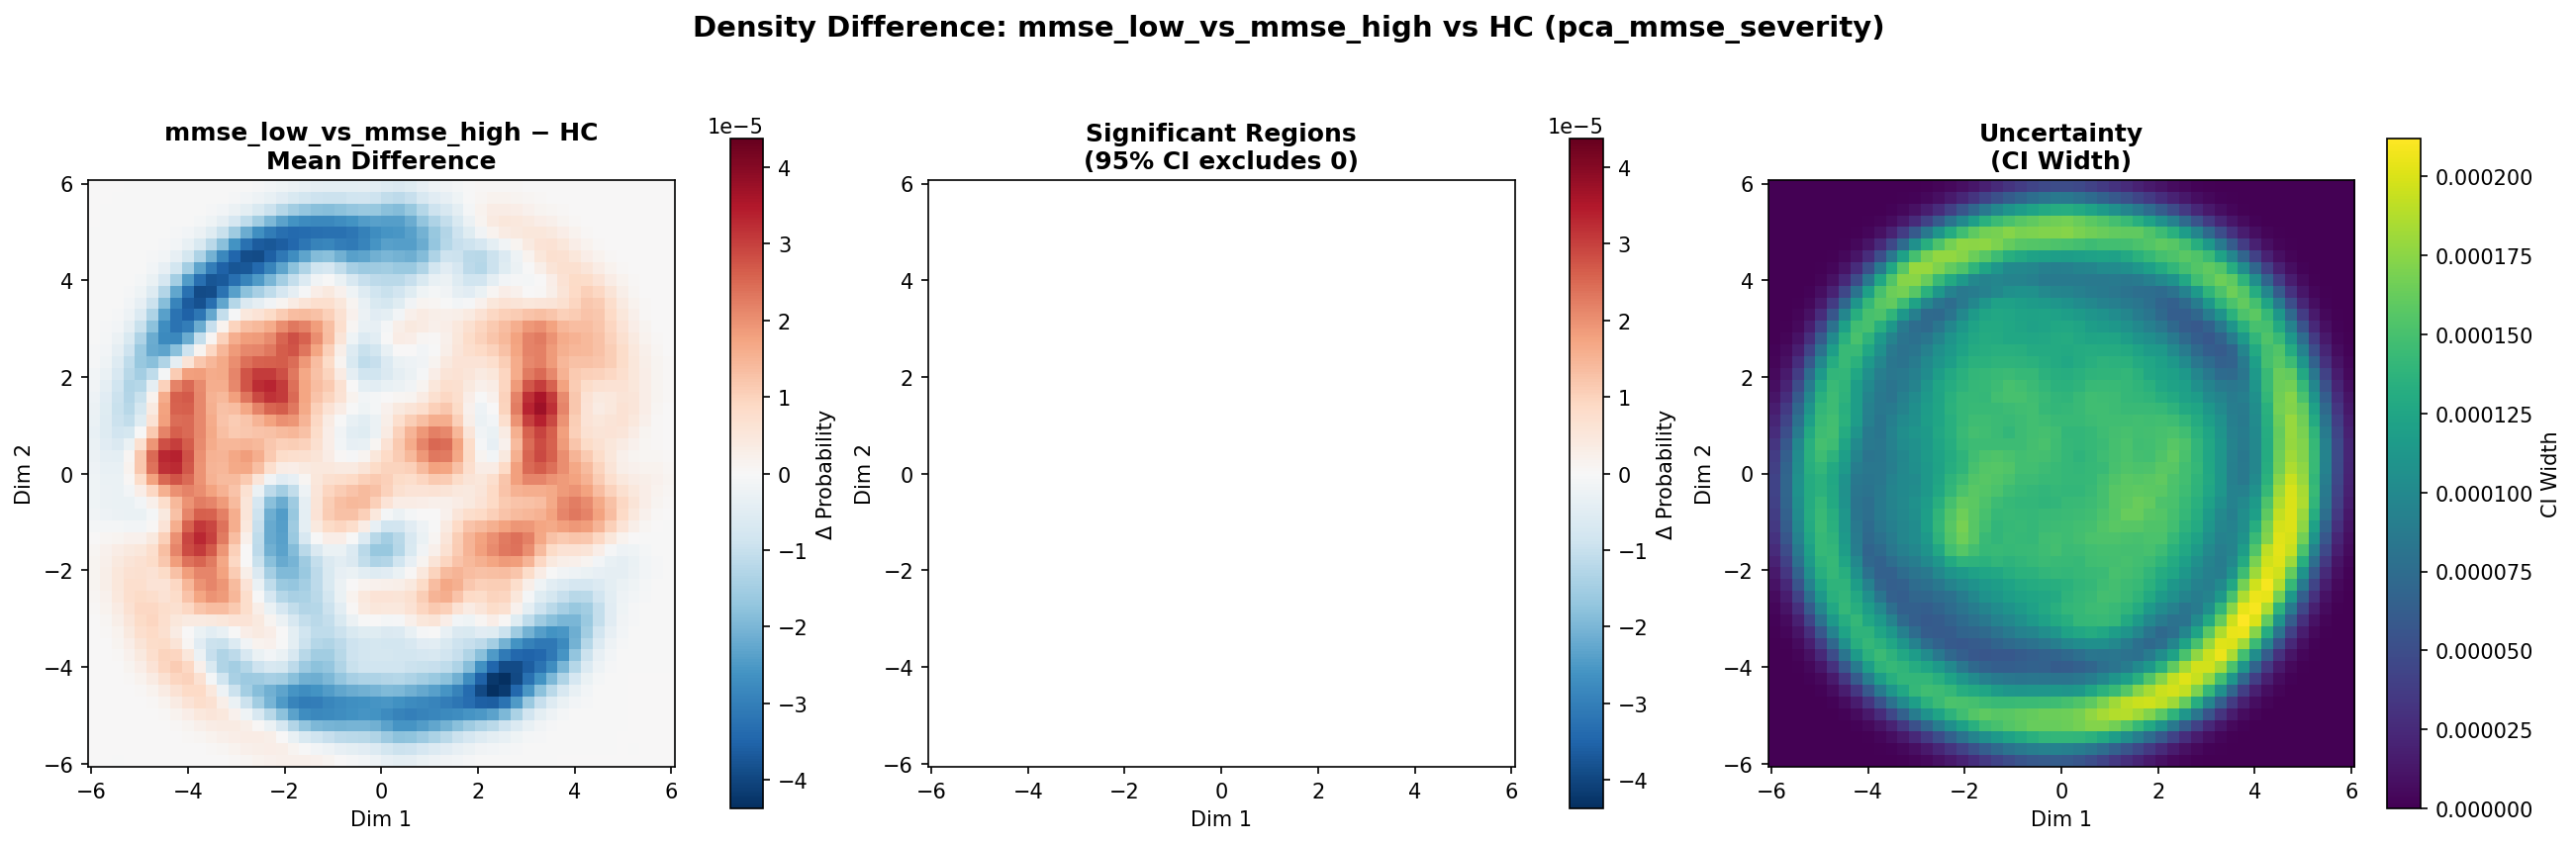
\includegraphics[width=\linewidth]{figures/paper2-wip/density_diff_ci_mmse_low_vs_mmse_high_pca_mmse_severity.png}
    \caption{Density difference: MMSE Low vs High.}
    \label{fig:mmse_density_low_high}
\end{figure}

\begin{figure}[H]
    \centering
    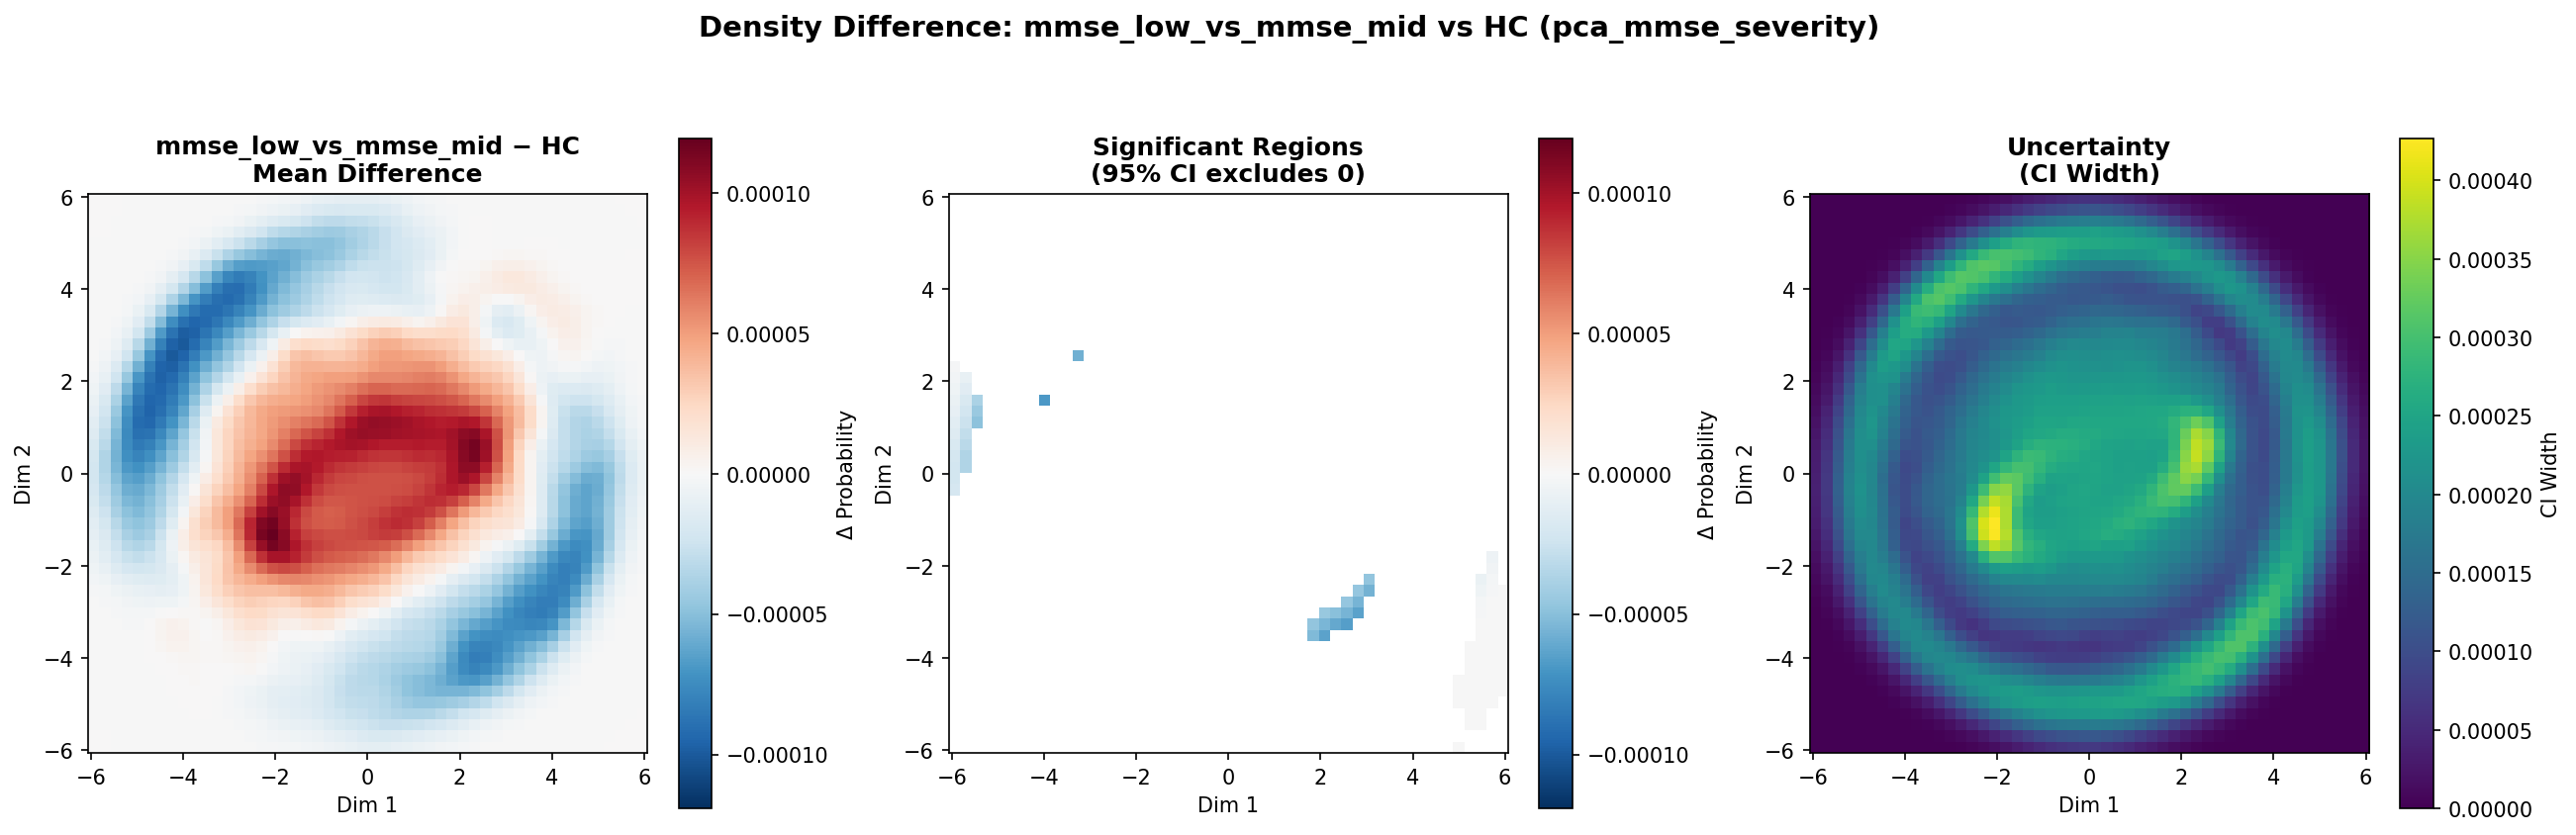
\includegraphics[width=\linewidth]{figures/paper2-wip/density_diff_ci_mmse_low_vs_mmse_mid_pca_mmse_severity.png}
    \caption{Density difference: MMSE Low vs Mid.}
    \label{fig:mmse_density_low_mid}
\end{figure}

\subsubsection{Streamlines by MMSE}

\begin{figure}[H]
    \centering
    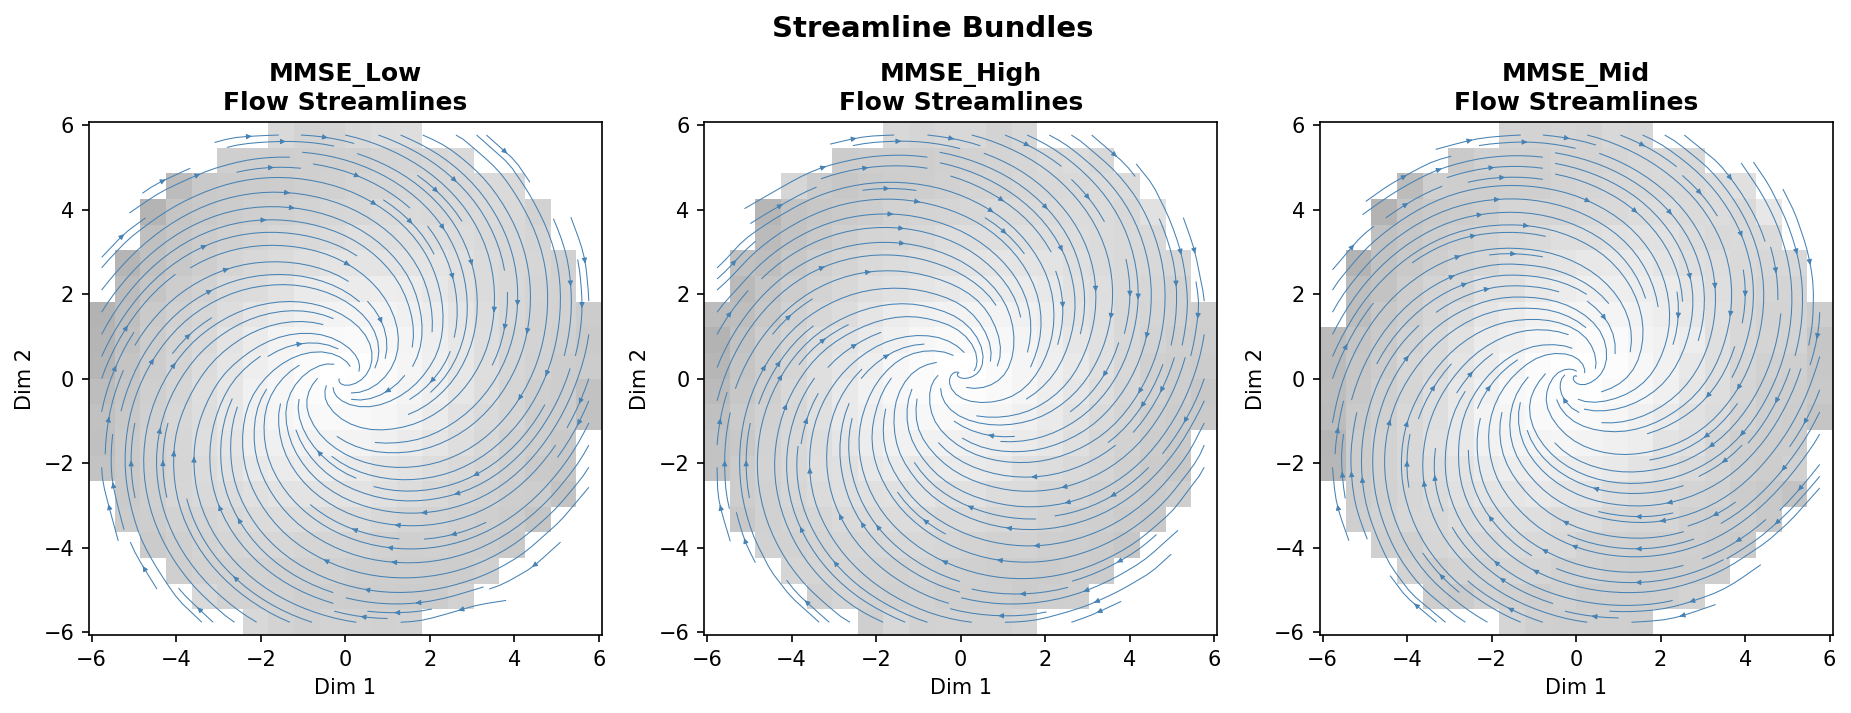
\includegraphics[width=\linewidth]{figures/paper2-wip/streamline_bundles_pca_mmse_severity.png}
    \caption{Streamline bundles by MMSE severity group.}
    \label{fig:mmse_streamlines}
\end{figure}

\subsection{Functional Impairment Stratification}

\subsubsection{Bootstrap Metrics}

\figref{fig:func_bootstrap} shows flow metrics stratified by functional impairment level.

\begin{figure}[H]
    \centering
    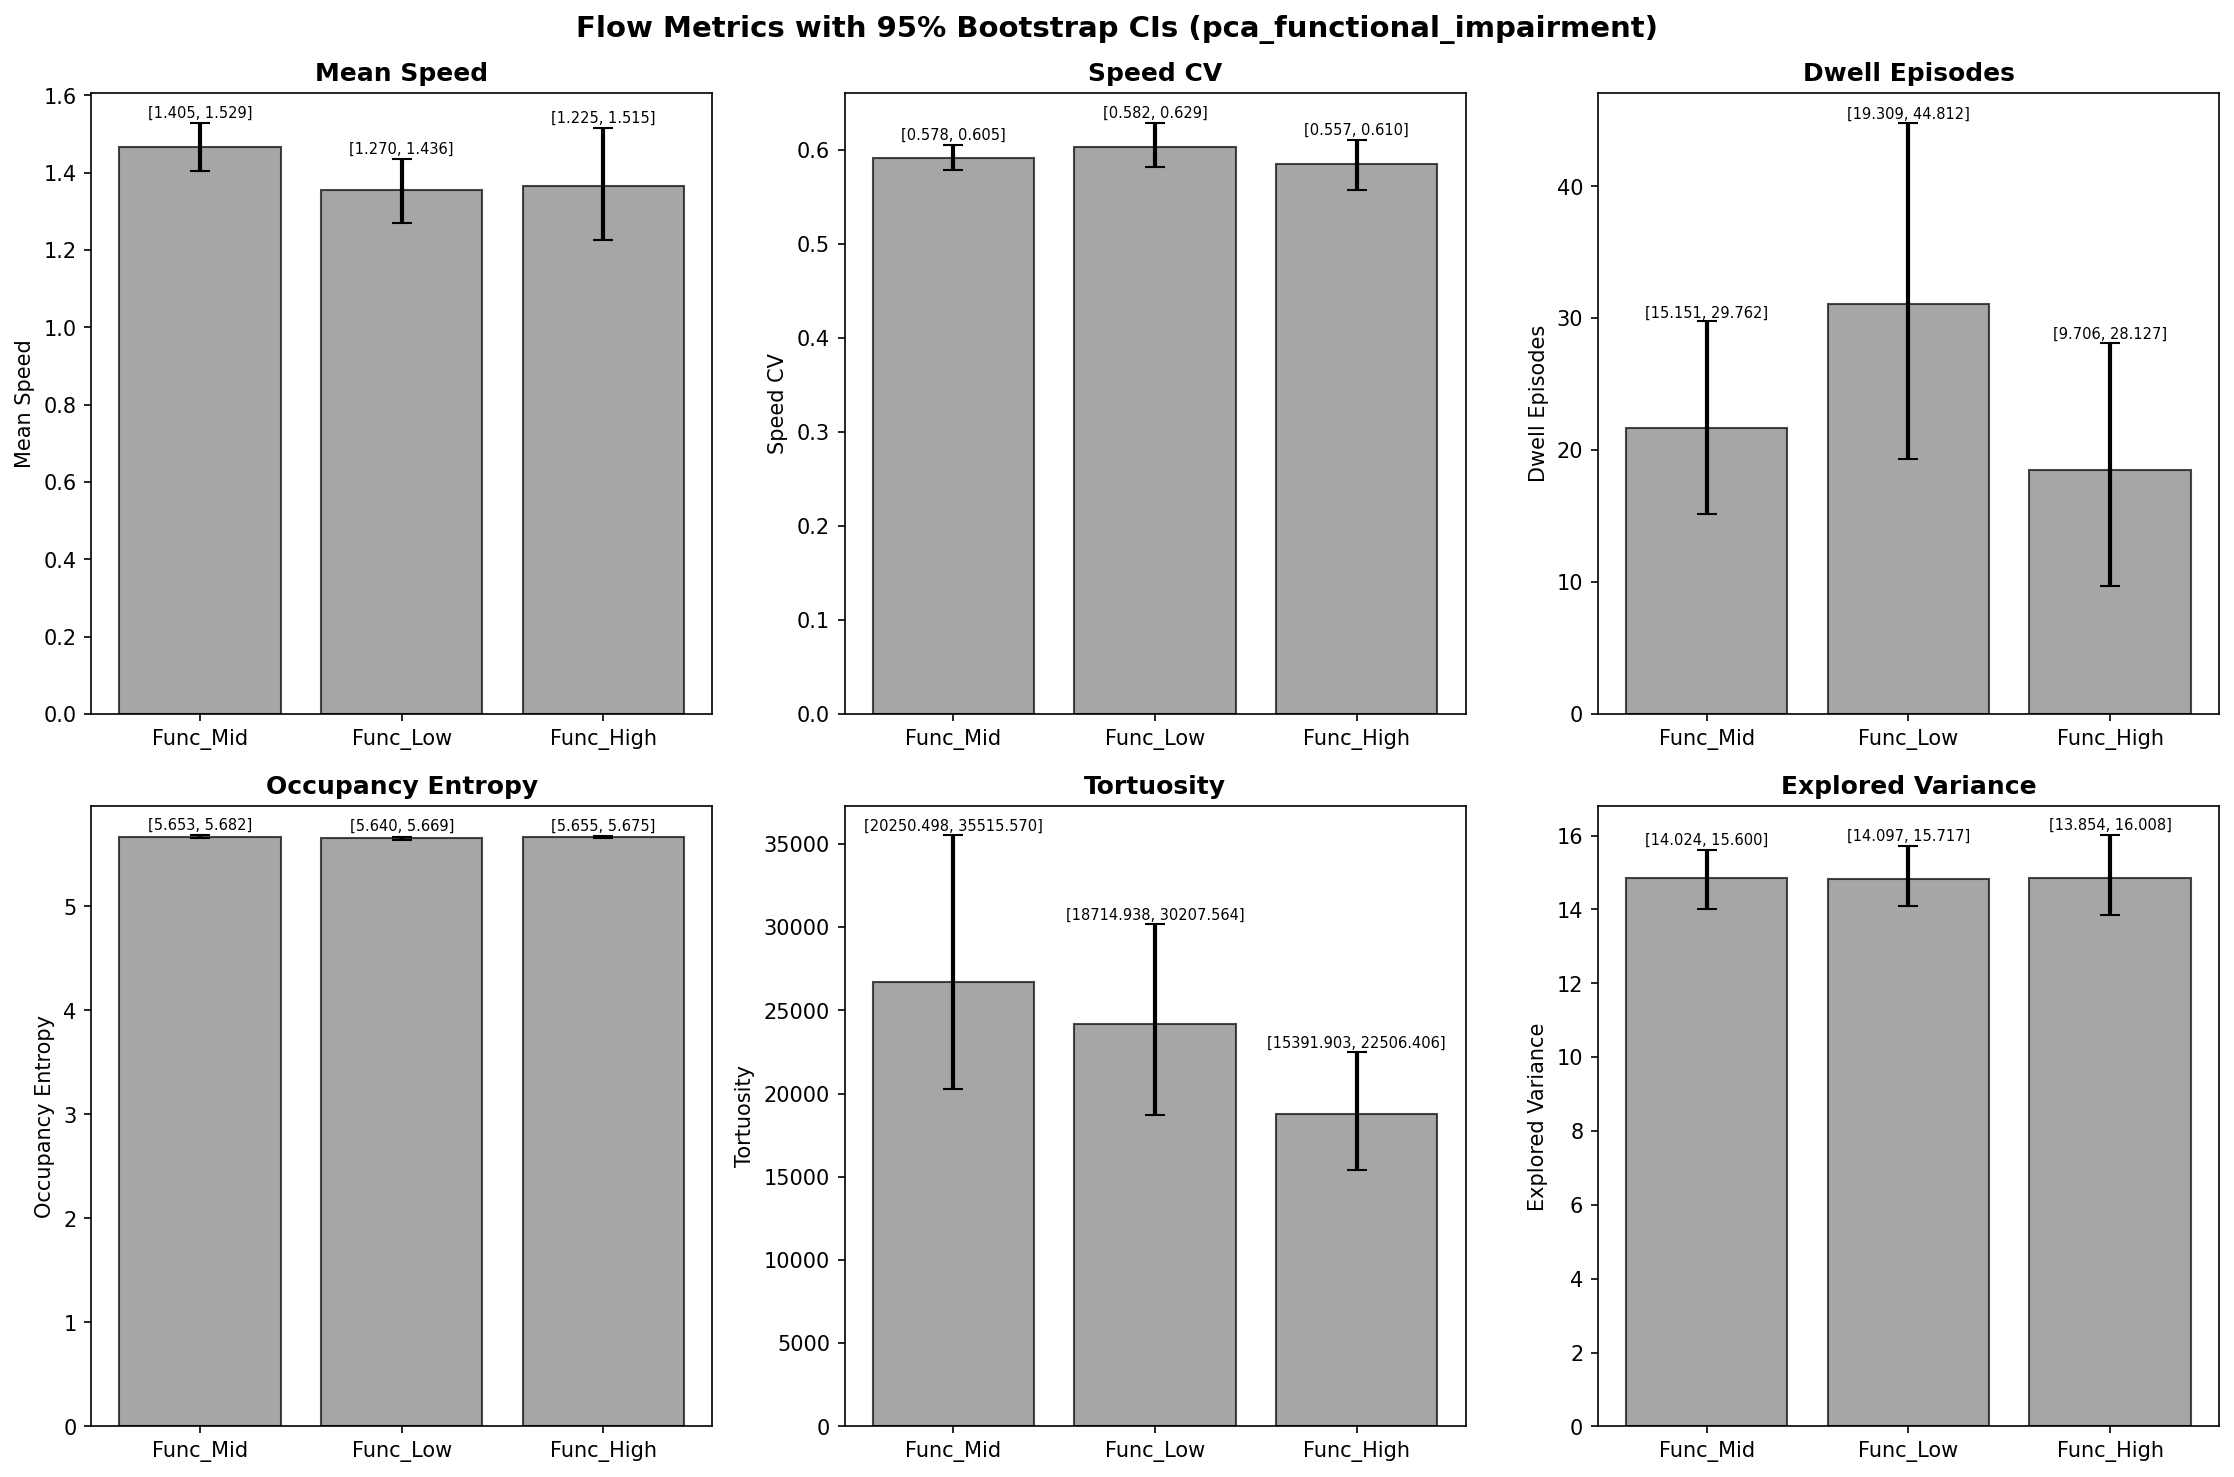
\includegraphics[width=\linewidth]{figures/paper2-wip/bootstrap_metrics_pca_functional_impairment.png}
    \caption{Bootstrap distributions of flow metrics stratified by functional impairment (Low = mild, Mid = moderate, High = severe impairment).}
    \label{fig:func_bootstrap}
\end{figure}

\textbf{Key findings by functional impairment}:
\begin{itemize}
    \item \textbf{Mean Speed}: Func Mid vs Low shows $d = 0.56$ [0.07, 1.08] --- moderate impairment associated with faster dynamics
    \item \textbf{Path Tortuosity}: Func Mid vs High shows $d = 0.50$ [0.04, 0.92] --- moderate impairment shows more complex paths than severe
\end{itemize}

\subsubsection{Flow Fields by Functional Impairment}

\begin{figure}[H]
    \centering
    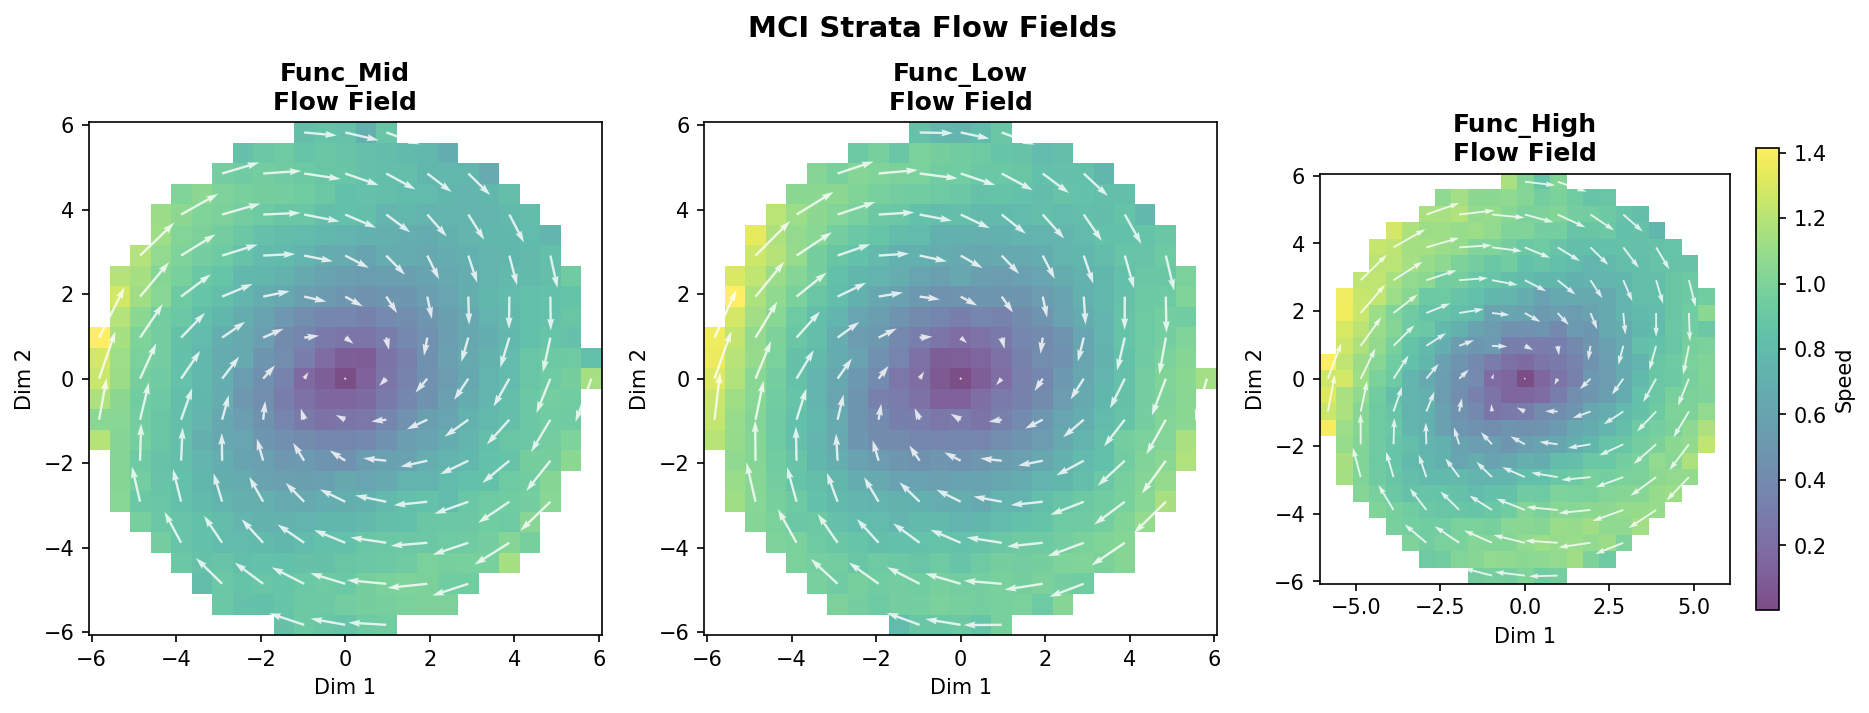
\includegraphics[width=\linewidth]{figures/paper2-wip/flow_fields_pca_functional_impairment.png}
    \caption{Flow fields stratified by functional impairment level.}
    \label{fig:func_flow_fields}
\end{figure}

\begin{figure}[H]
    \centering
    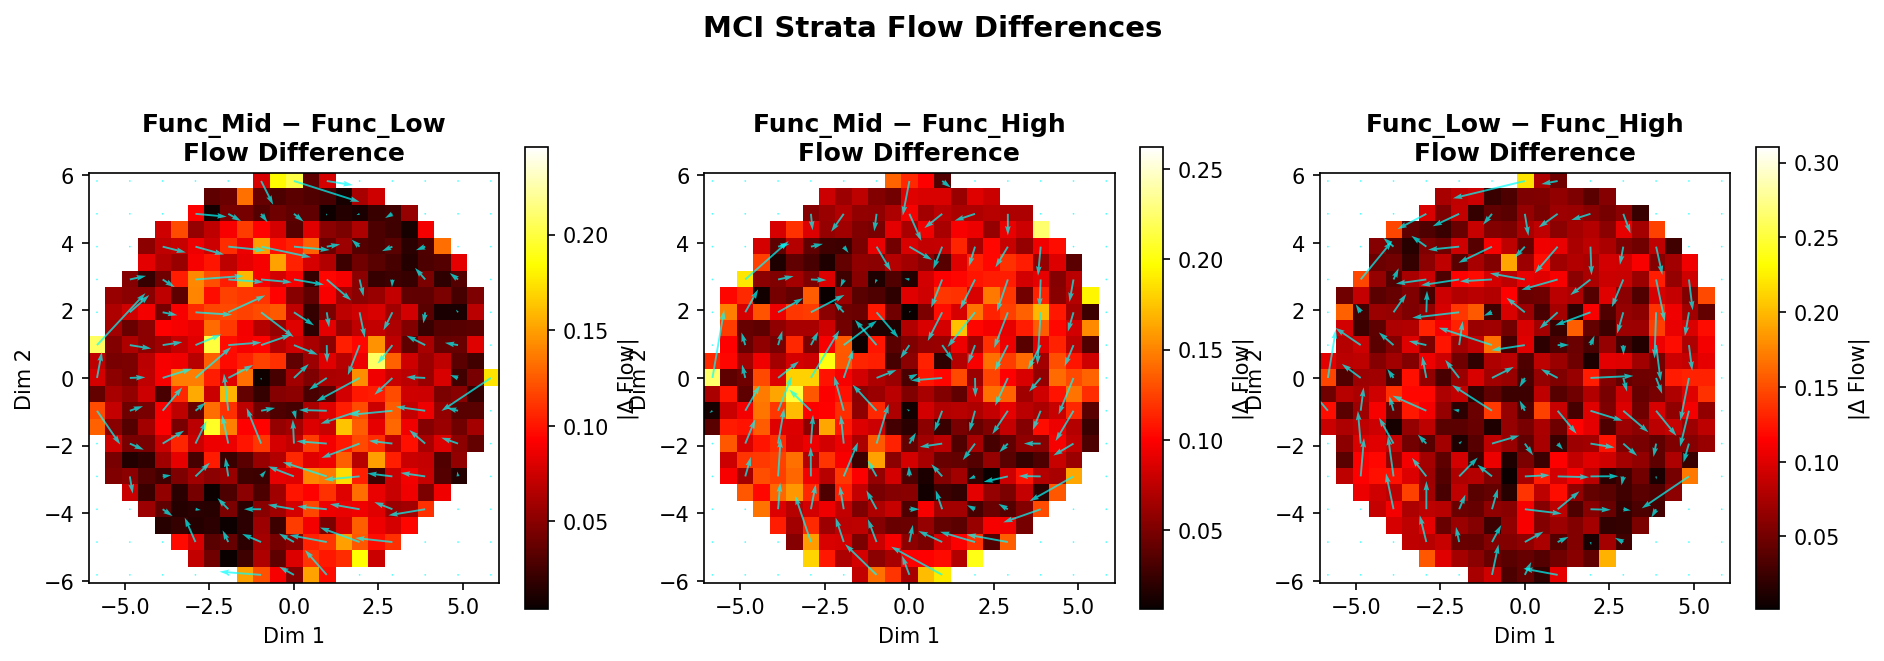
\includegraphics[width=\linewidth]{figures/paper2-wip/flow_difference_pca_functional_impairment.png}
    \caption{Flow field differences between functional impairment groups.}
    \label{fig:func_flow_diff}
\end{figure}

\subsubsection{Radial Profiles and Dwell Fields}

\begin{figure}[H]
    \centering
    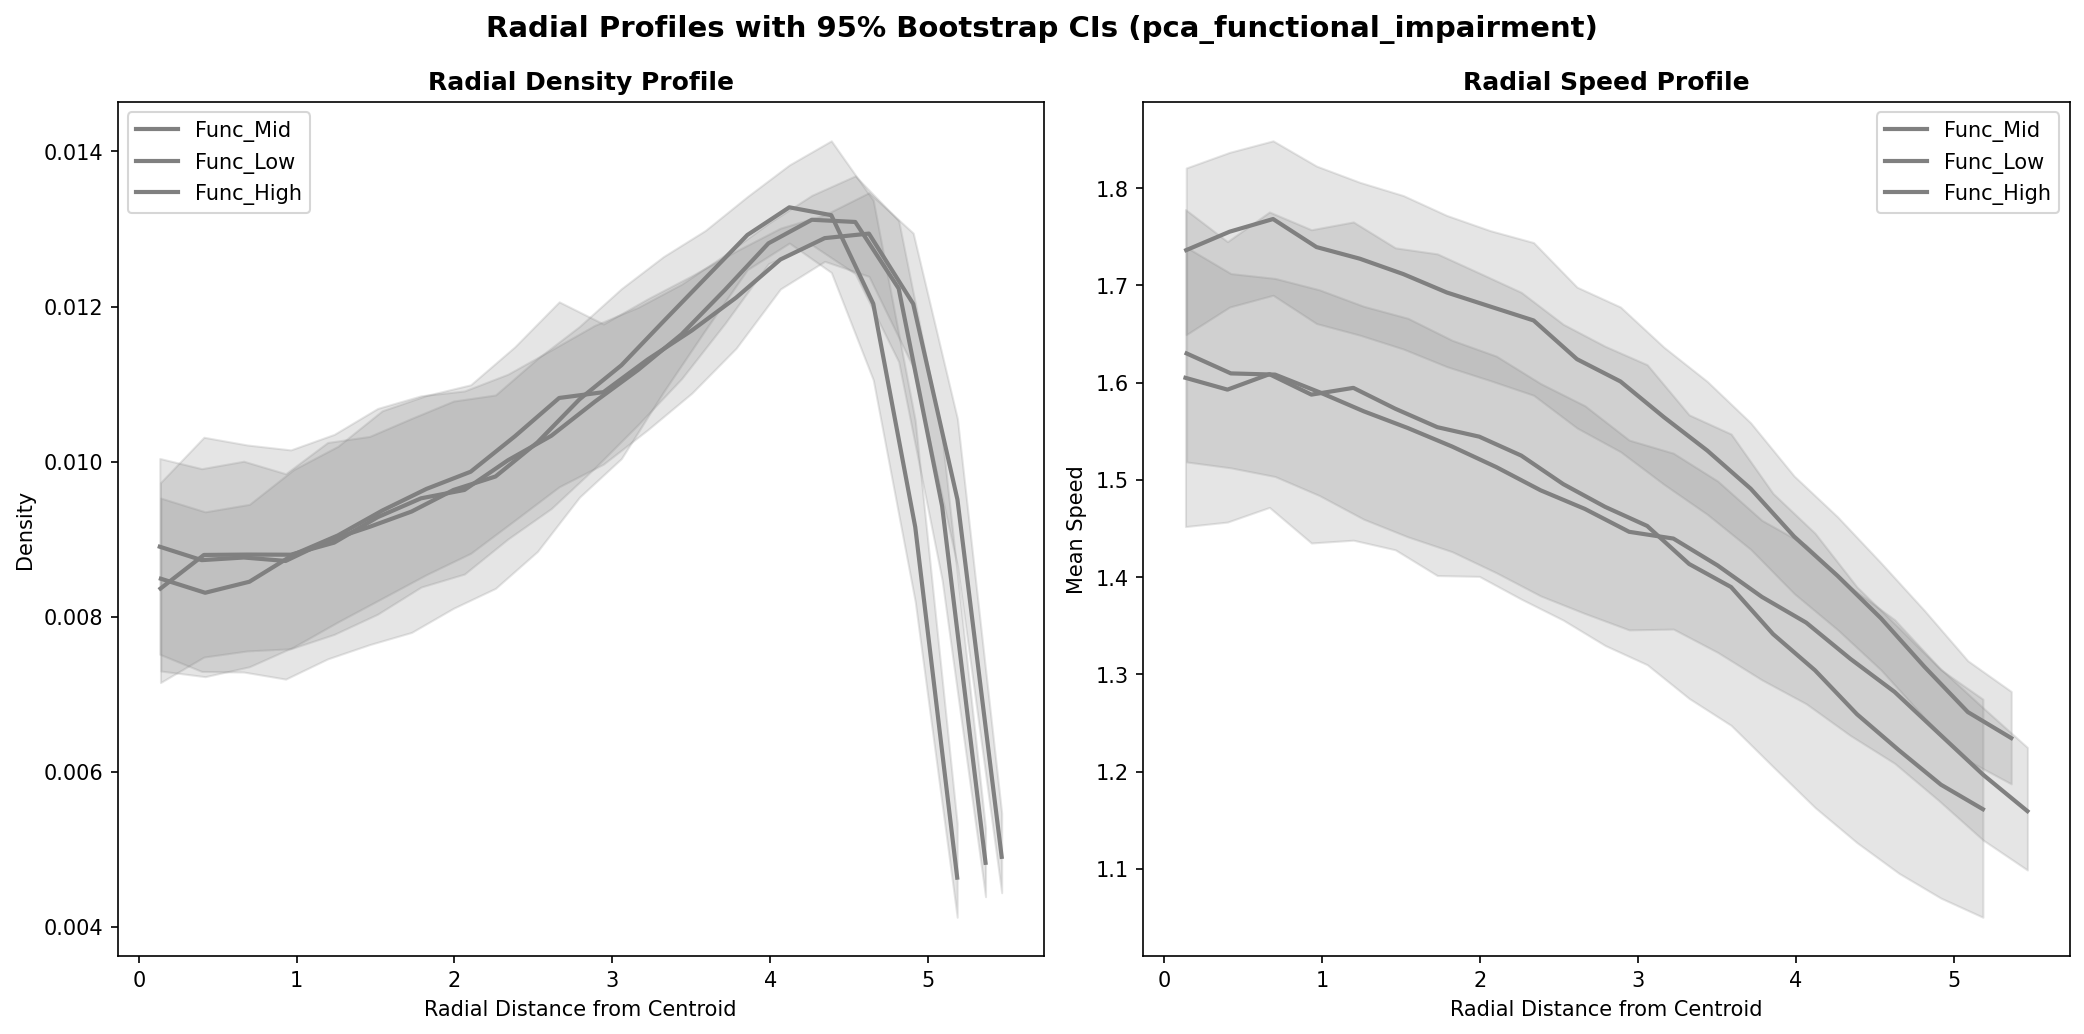
\includegraphics[width=\linewidth]{figures/paper2-wip/radial_profiles_pca_functional_impairment.png}
    \caption{Radial profiles by functional impairment.}
    \label{fig:func_radial}
\end{figure}

\begin{figure}[H]
    \centering
    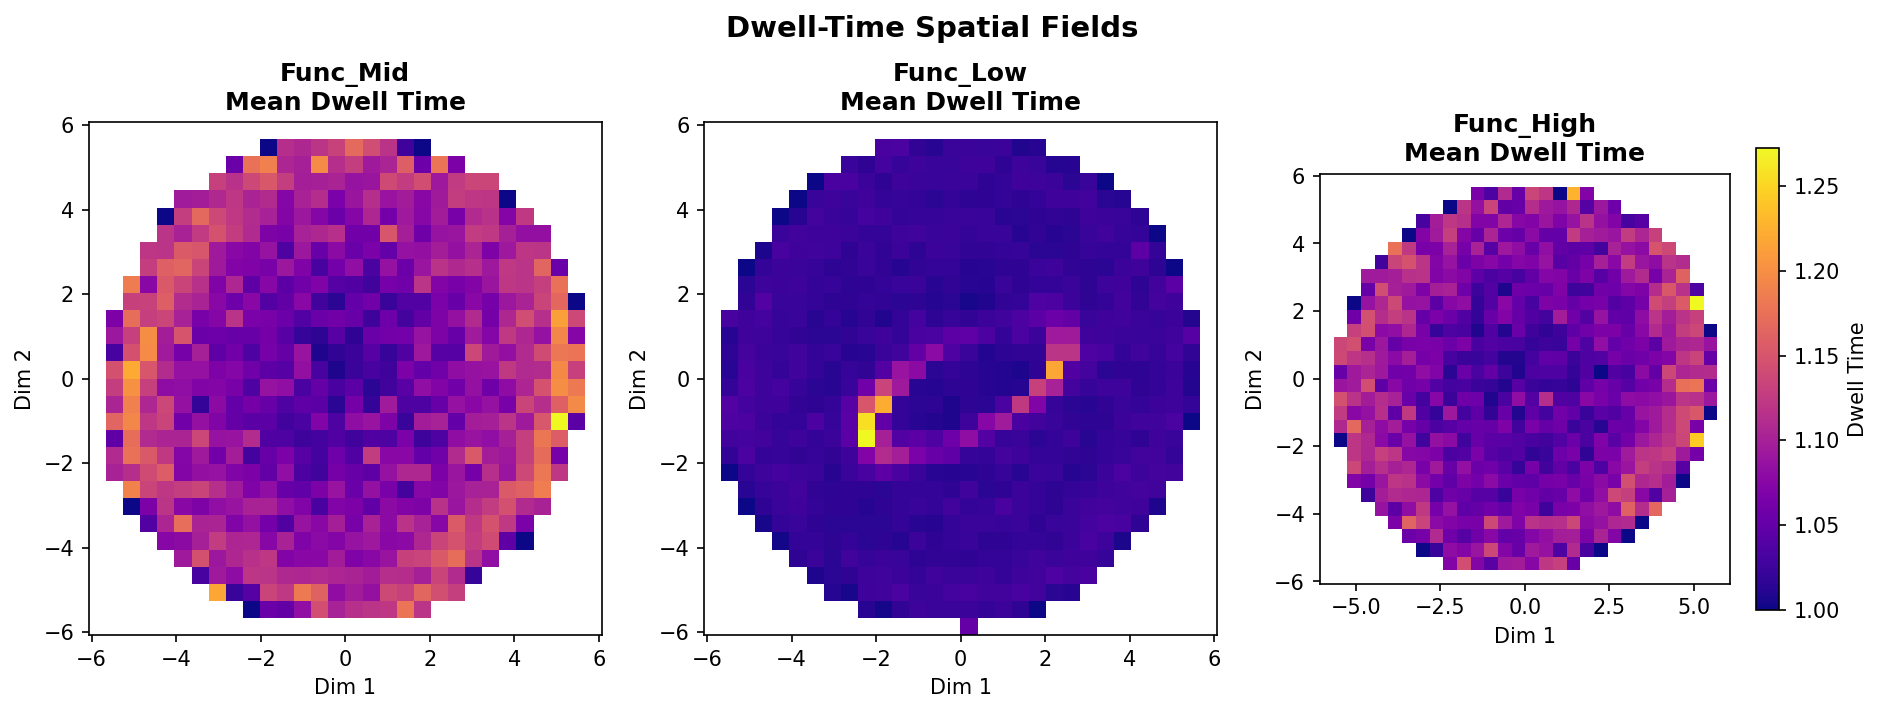
\includegraphics[width=\linewidth]{figures/paper2-wip/dwell_time_fields_pca_functional_impairment.png}
    \caption{Dwell time fields by functional impairment.}
    \label{fig:func_dwell}
\end{figure}

\subsubsection{Density Differences}

\begin{figure}[H]
    \centering
    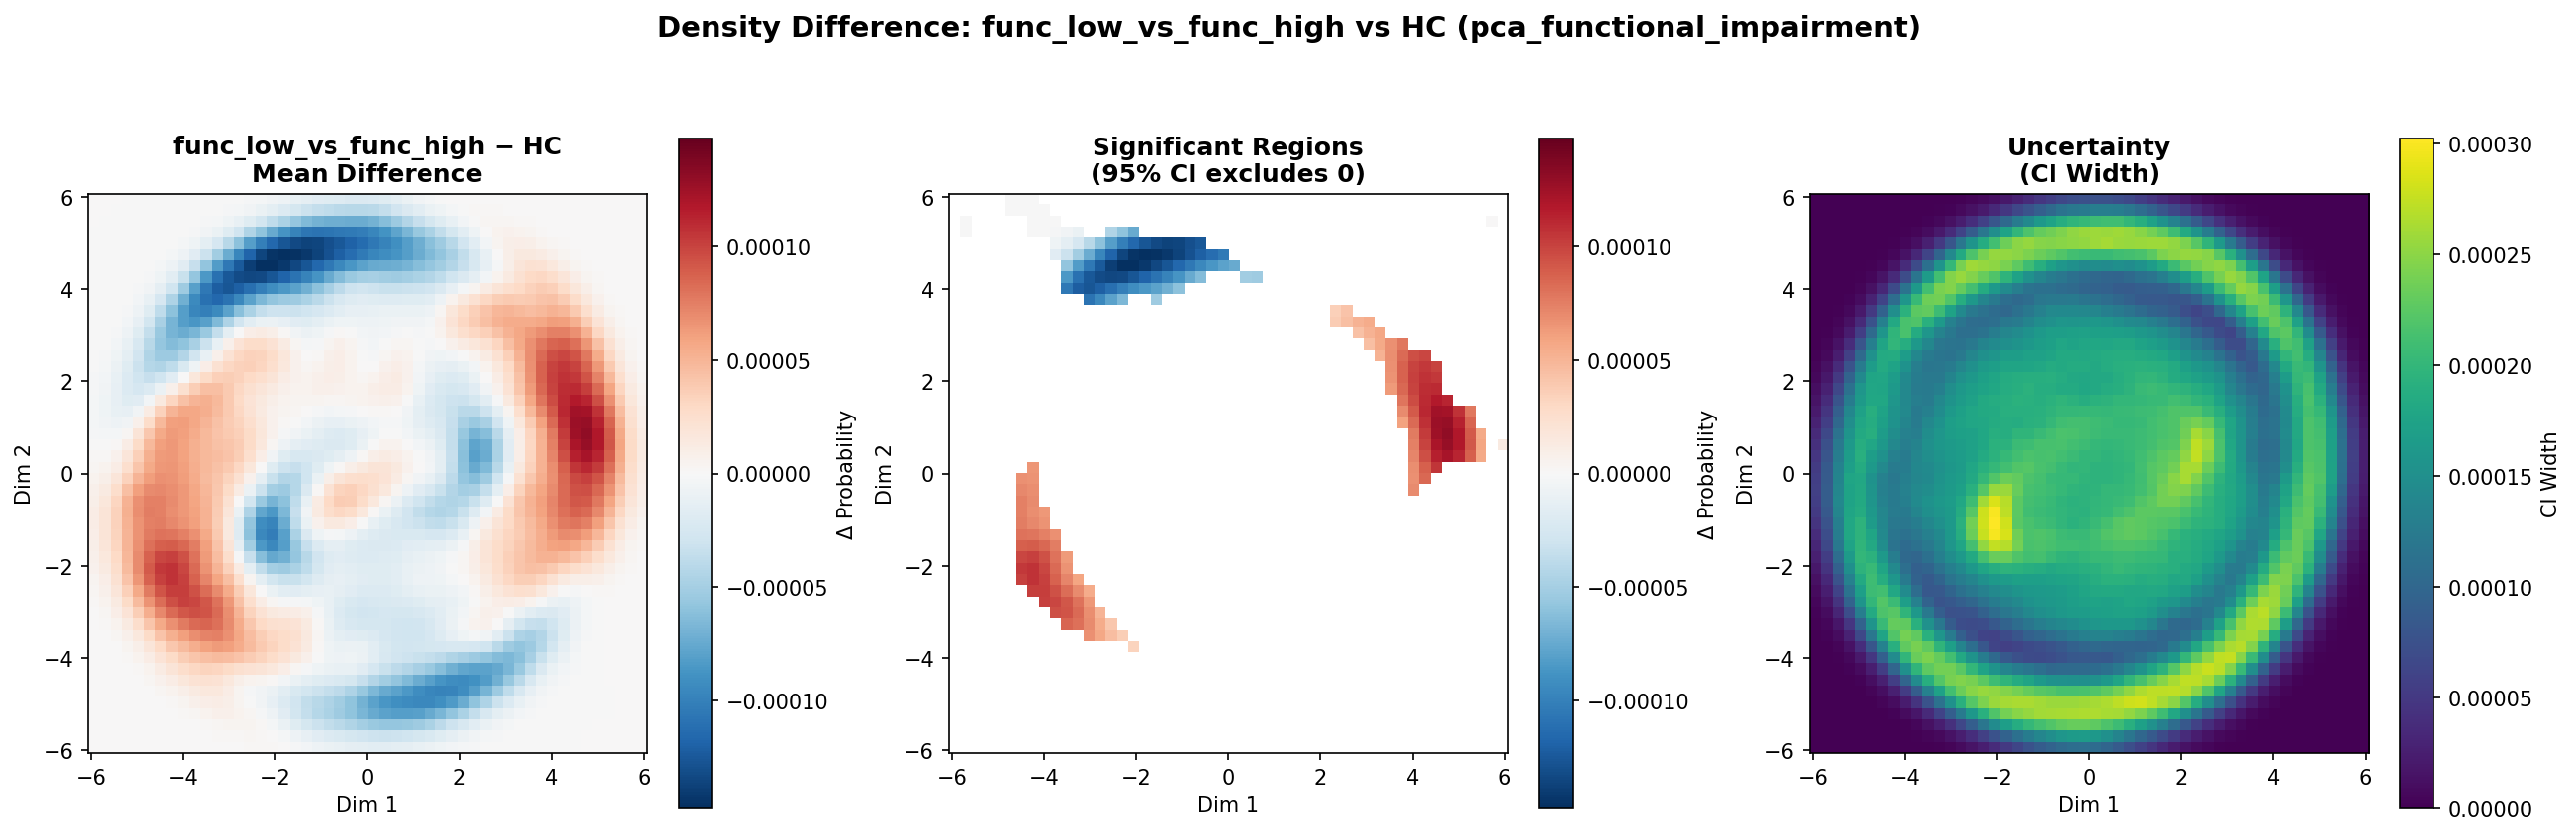
\includegraphics[width=\linewidth]{figures/paper2-wip/density_diff_ci_func_low_vs_func_high_pca_functional_impairment.png}
    \caption{Density difference: Functional Low vs High.}
    \label{fig:func_density_low_high}
\end{figure}

\begin{figure}[H]
    \centering
    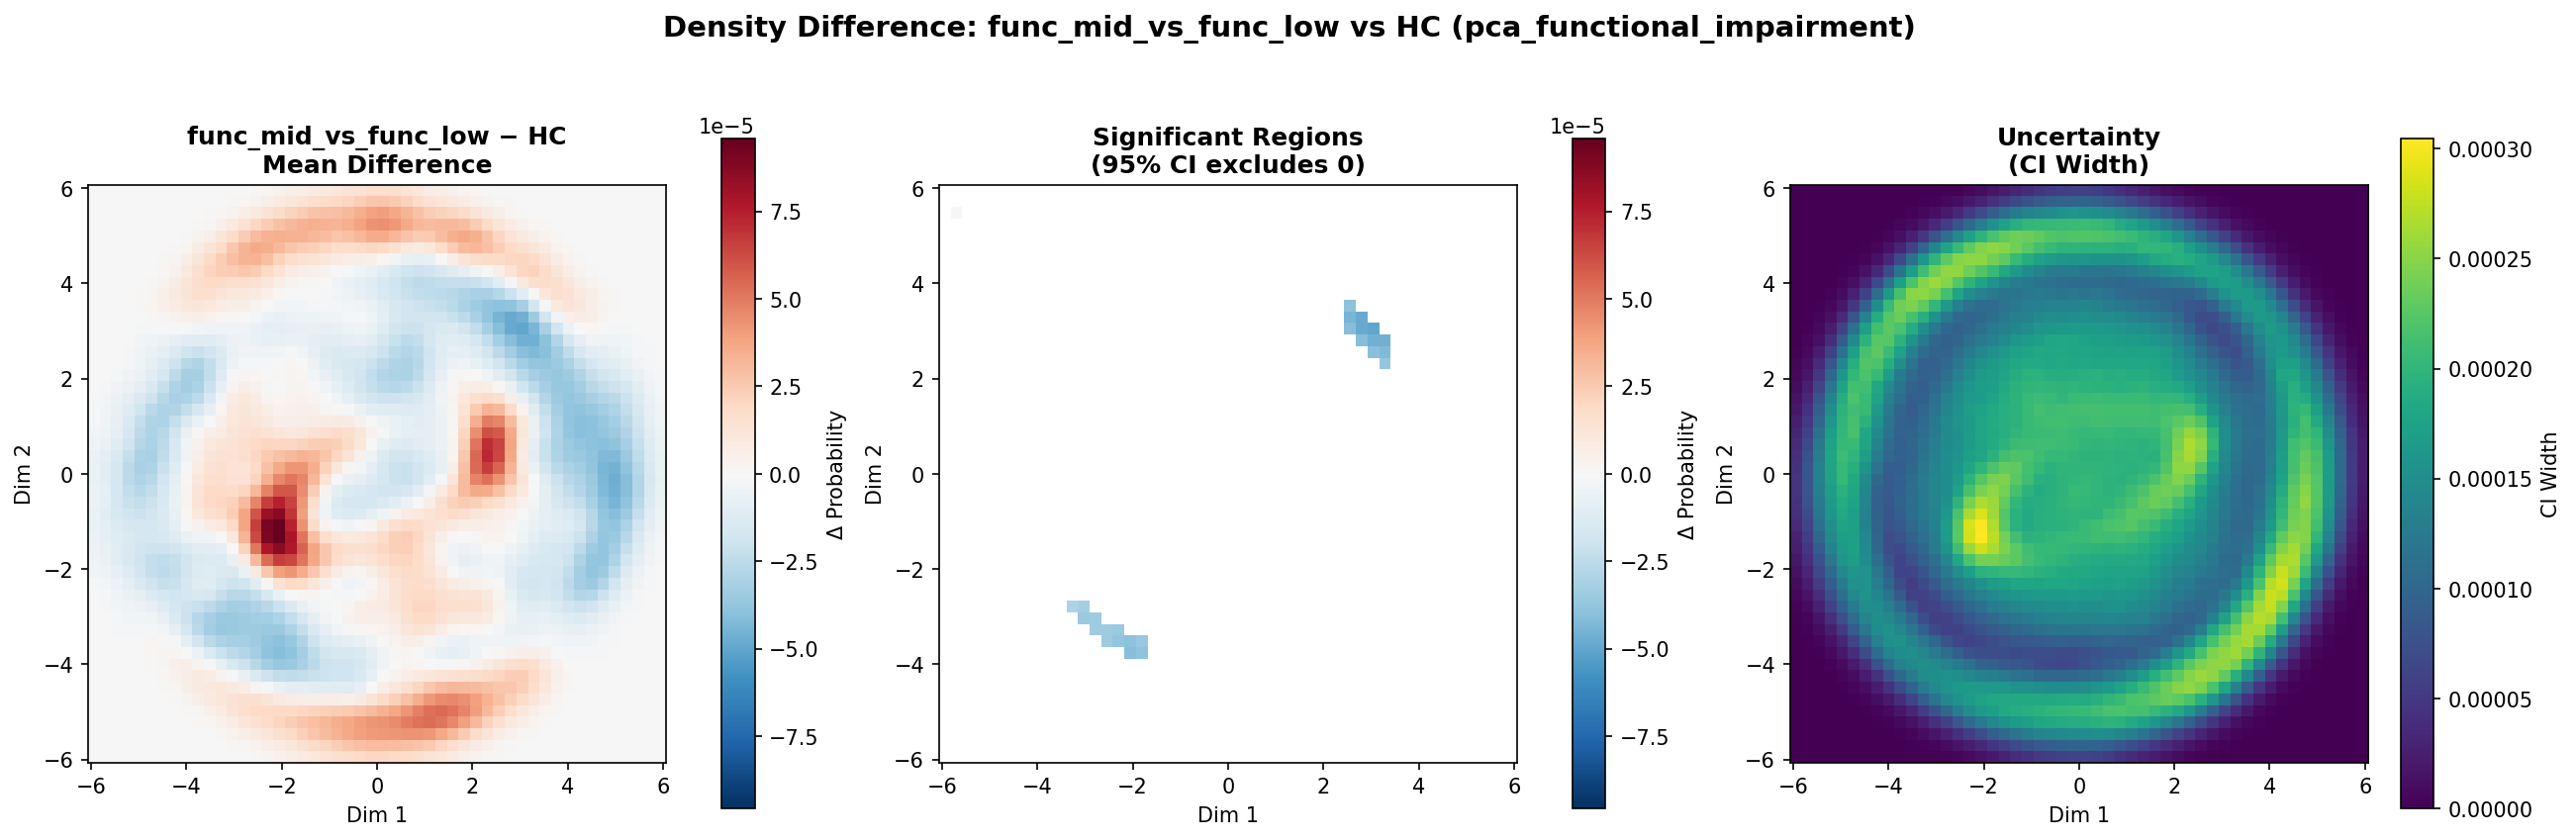
\includegraphics[width=\linewidth]{figures/paper2-wip/density_diff_ci_func_mid_vs_func_low_pca_functional_impairment.png}
    \caption{Density difference: Functional Mid vs Low.}
    \label{fig:func_density_mid_low}
\end{figure}

\subsubsection{Streamlines by Functional Impairment}

\begin{figure}[H]
    \centering
    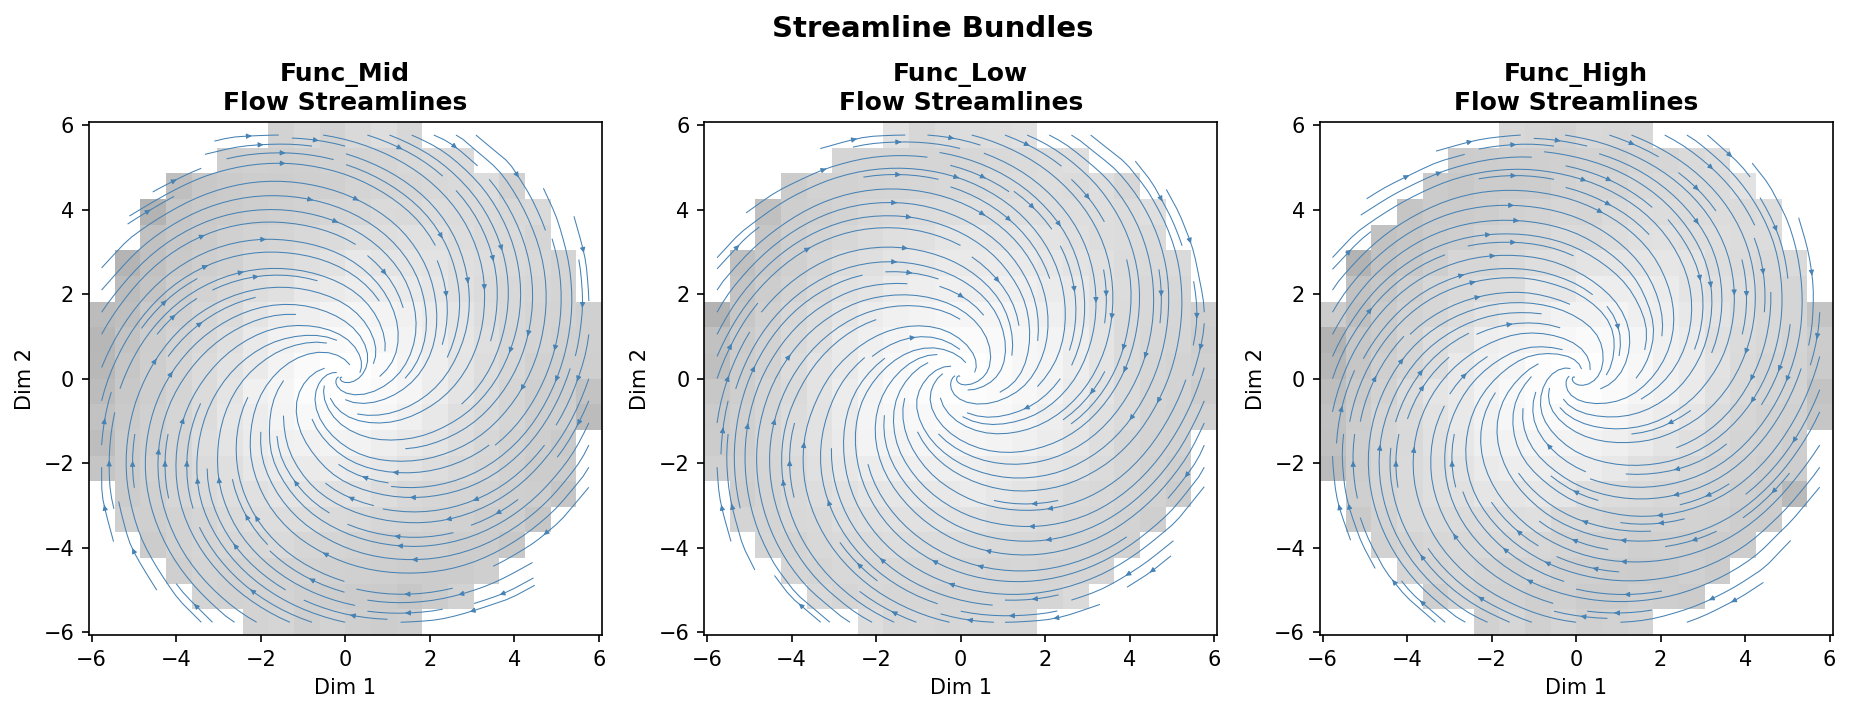
\includegraphics[width=\linewidth]{figures/paper2-wip/streamline_bundles_pca_functional_impairment.png}
    \caption{Streamline bundles by functional impairment level.}
    \label{fig:func_streamlines}
\end{figure}

\subsection{ROI Power Analysis}

We also examined regional power differences across subtypes.

\begin{figure}[H]
    \centering
    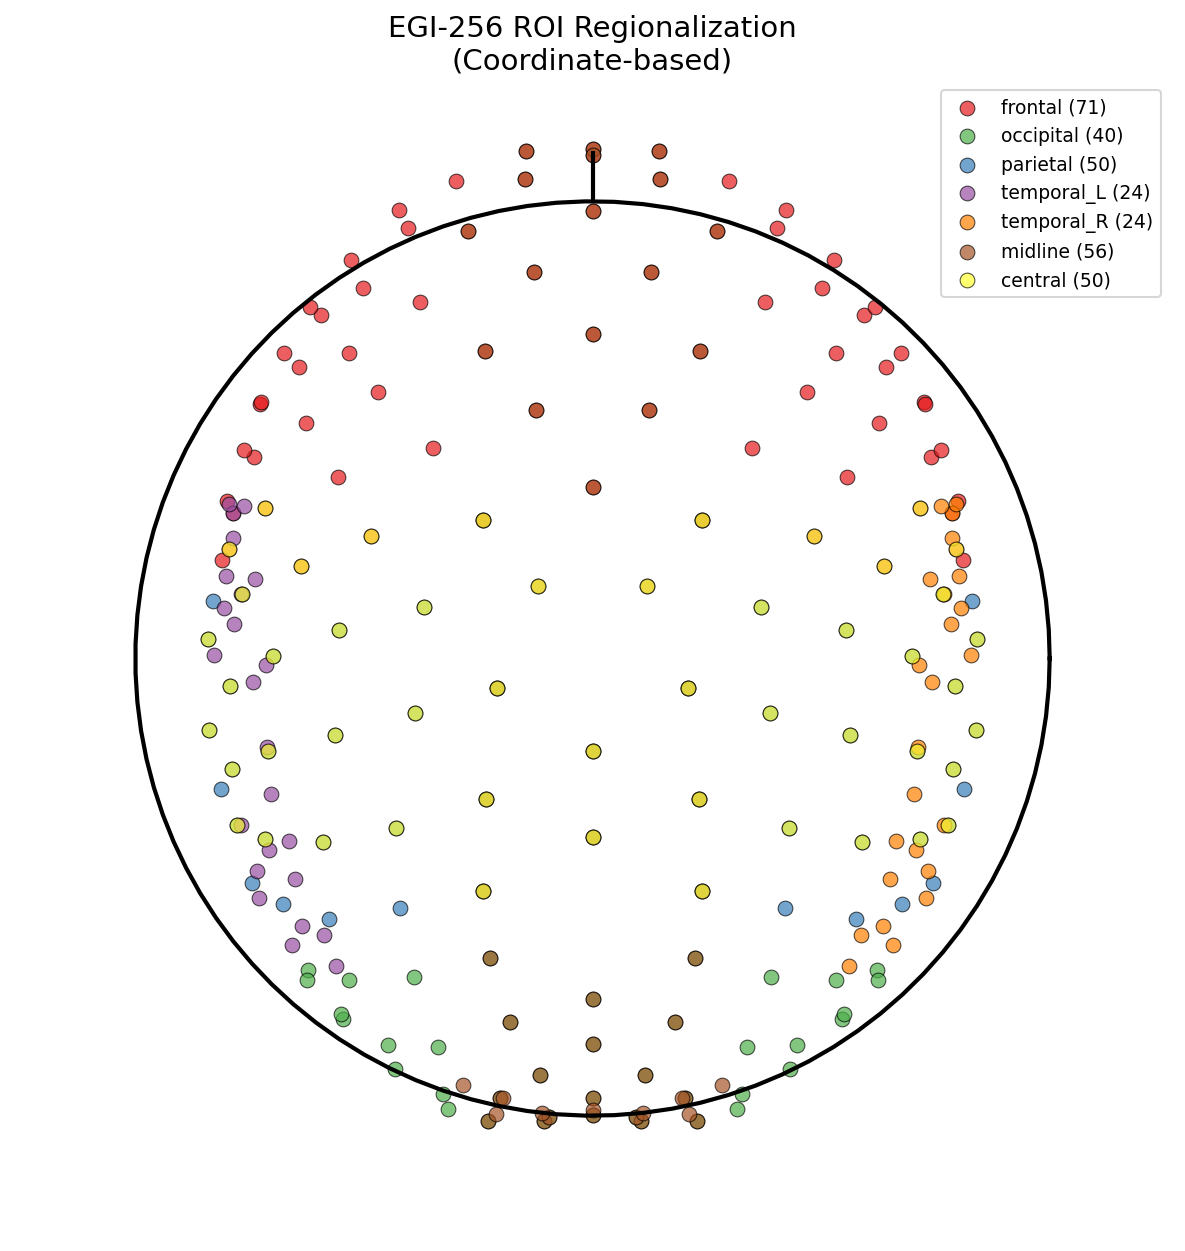
\includegraphics[width=0.8\linewidth]{figures/paper2-wip/roi_visualization.png}
    \caption{Regions of interest (ROIs) used for power analysis.}
    \label{fig:roi_viz}
\end{figure}

\begin{figure}[H]
    \centering
    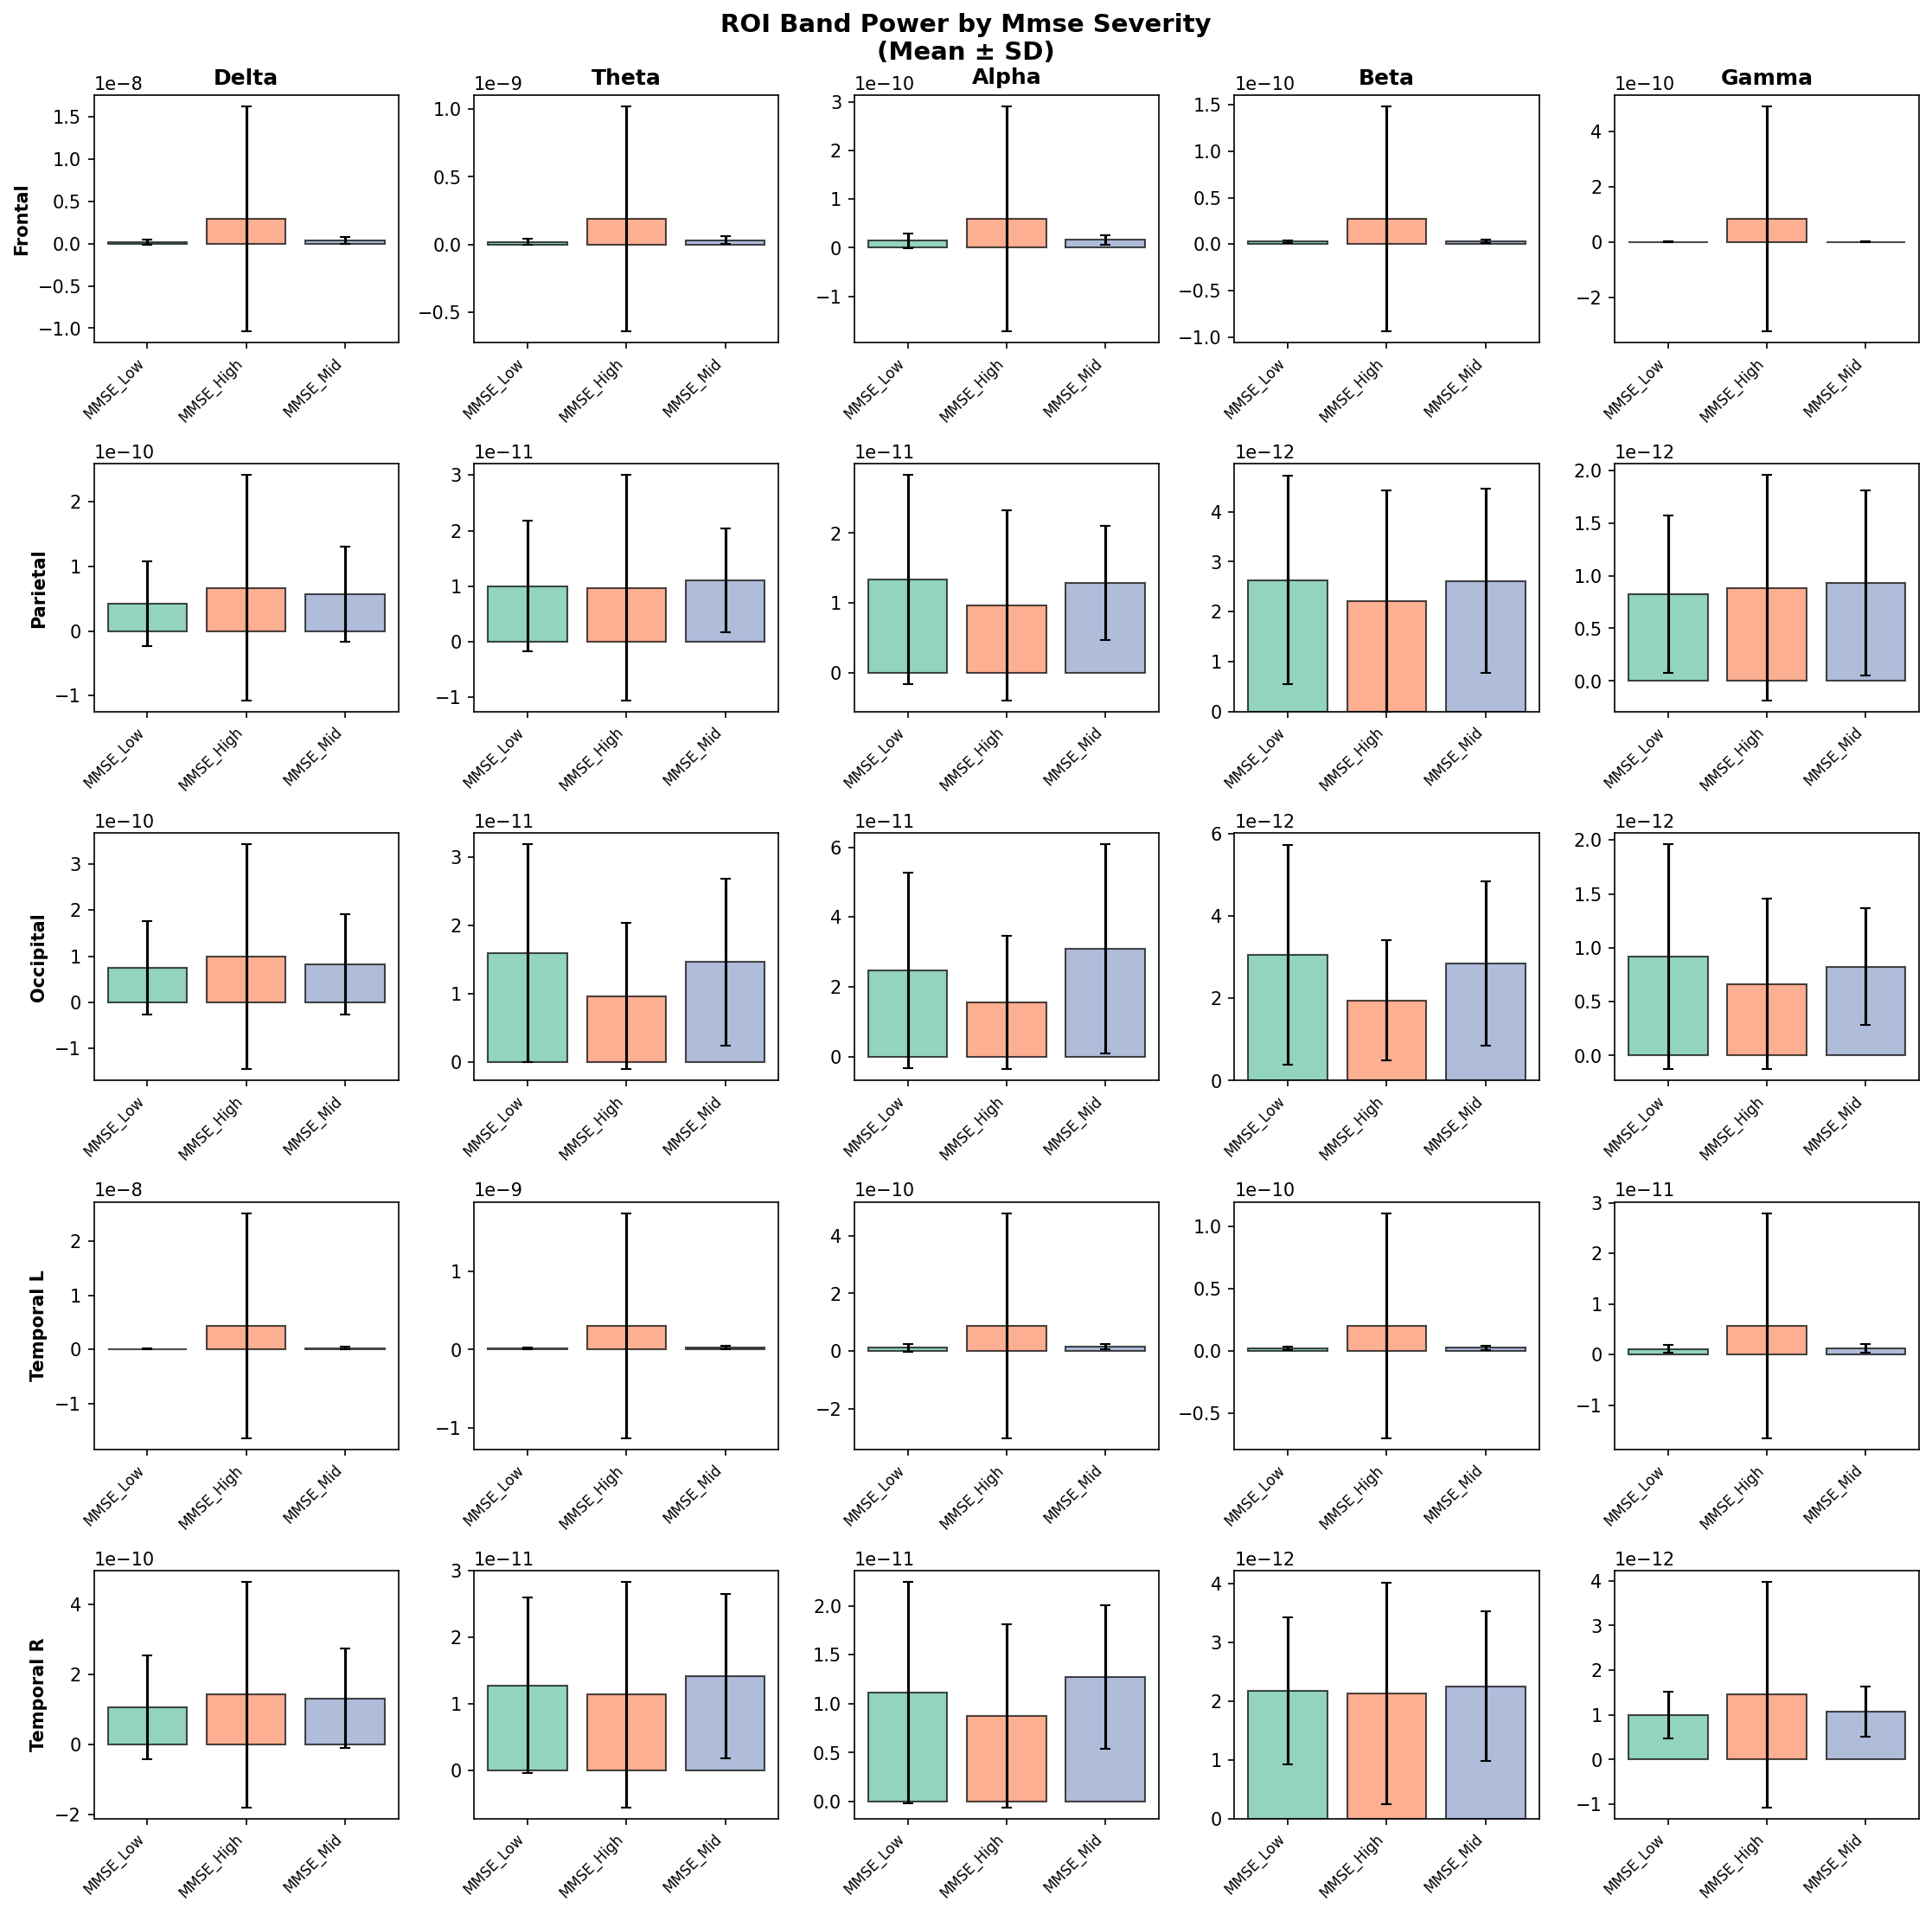
\includegraphics[width=\linewidth]{figures/paper2-wip/roi_power_comparison_mmse_severity.png}
    \caption{ROI power comparison by MMSE severity.}
    \label{fig:roi_mmse}
\end{figure}

\begin{figure}[H]
    \centering
    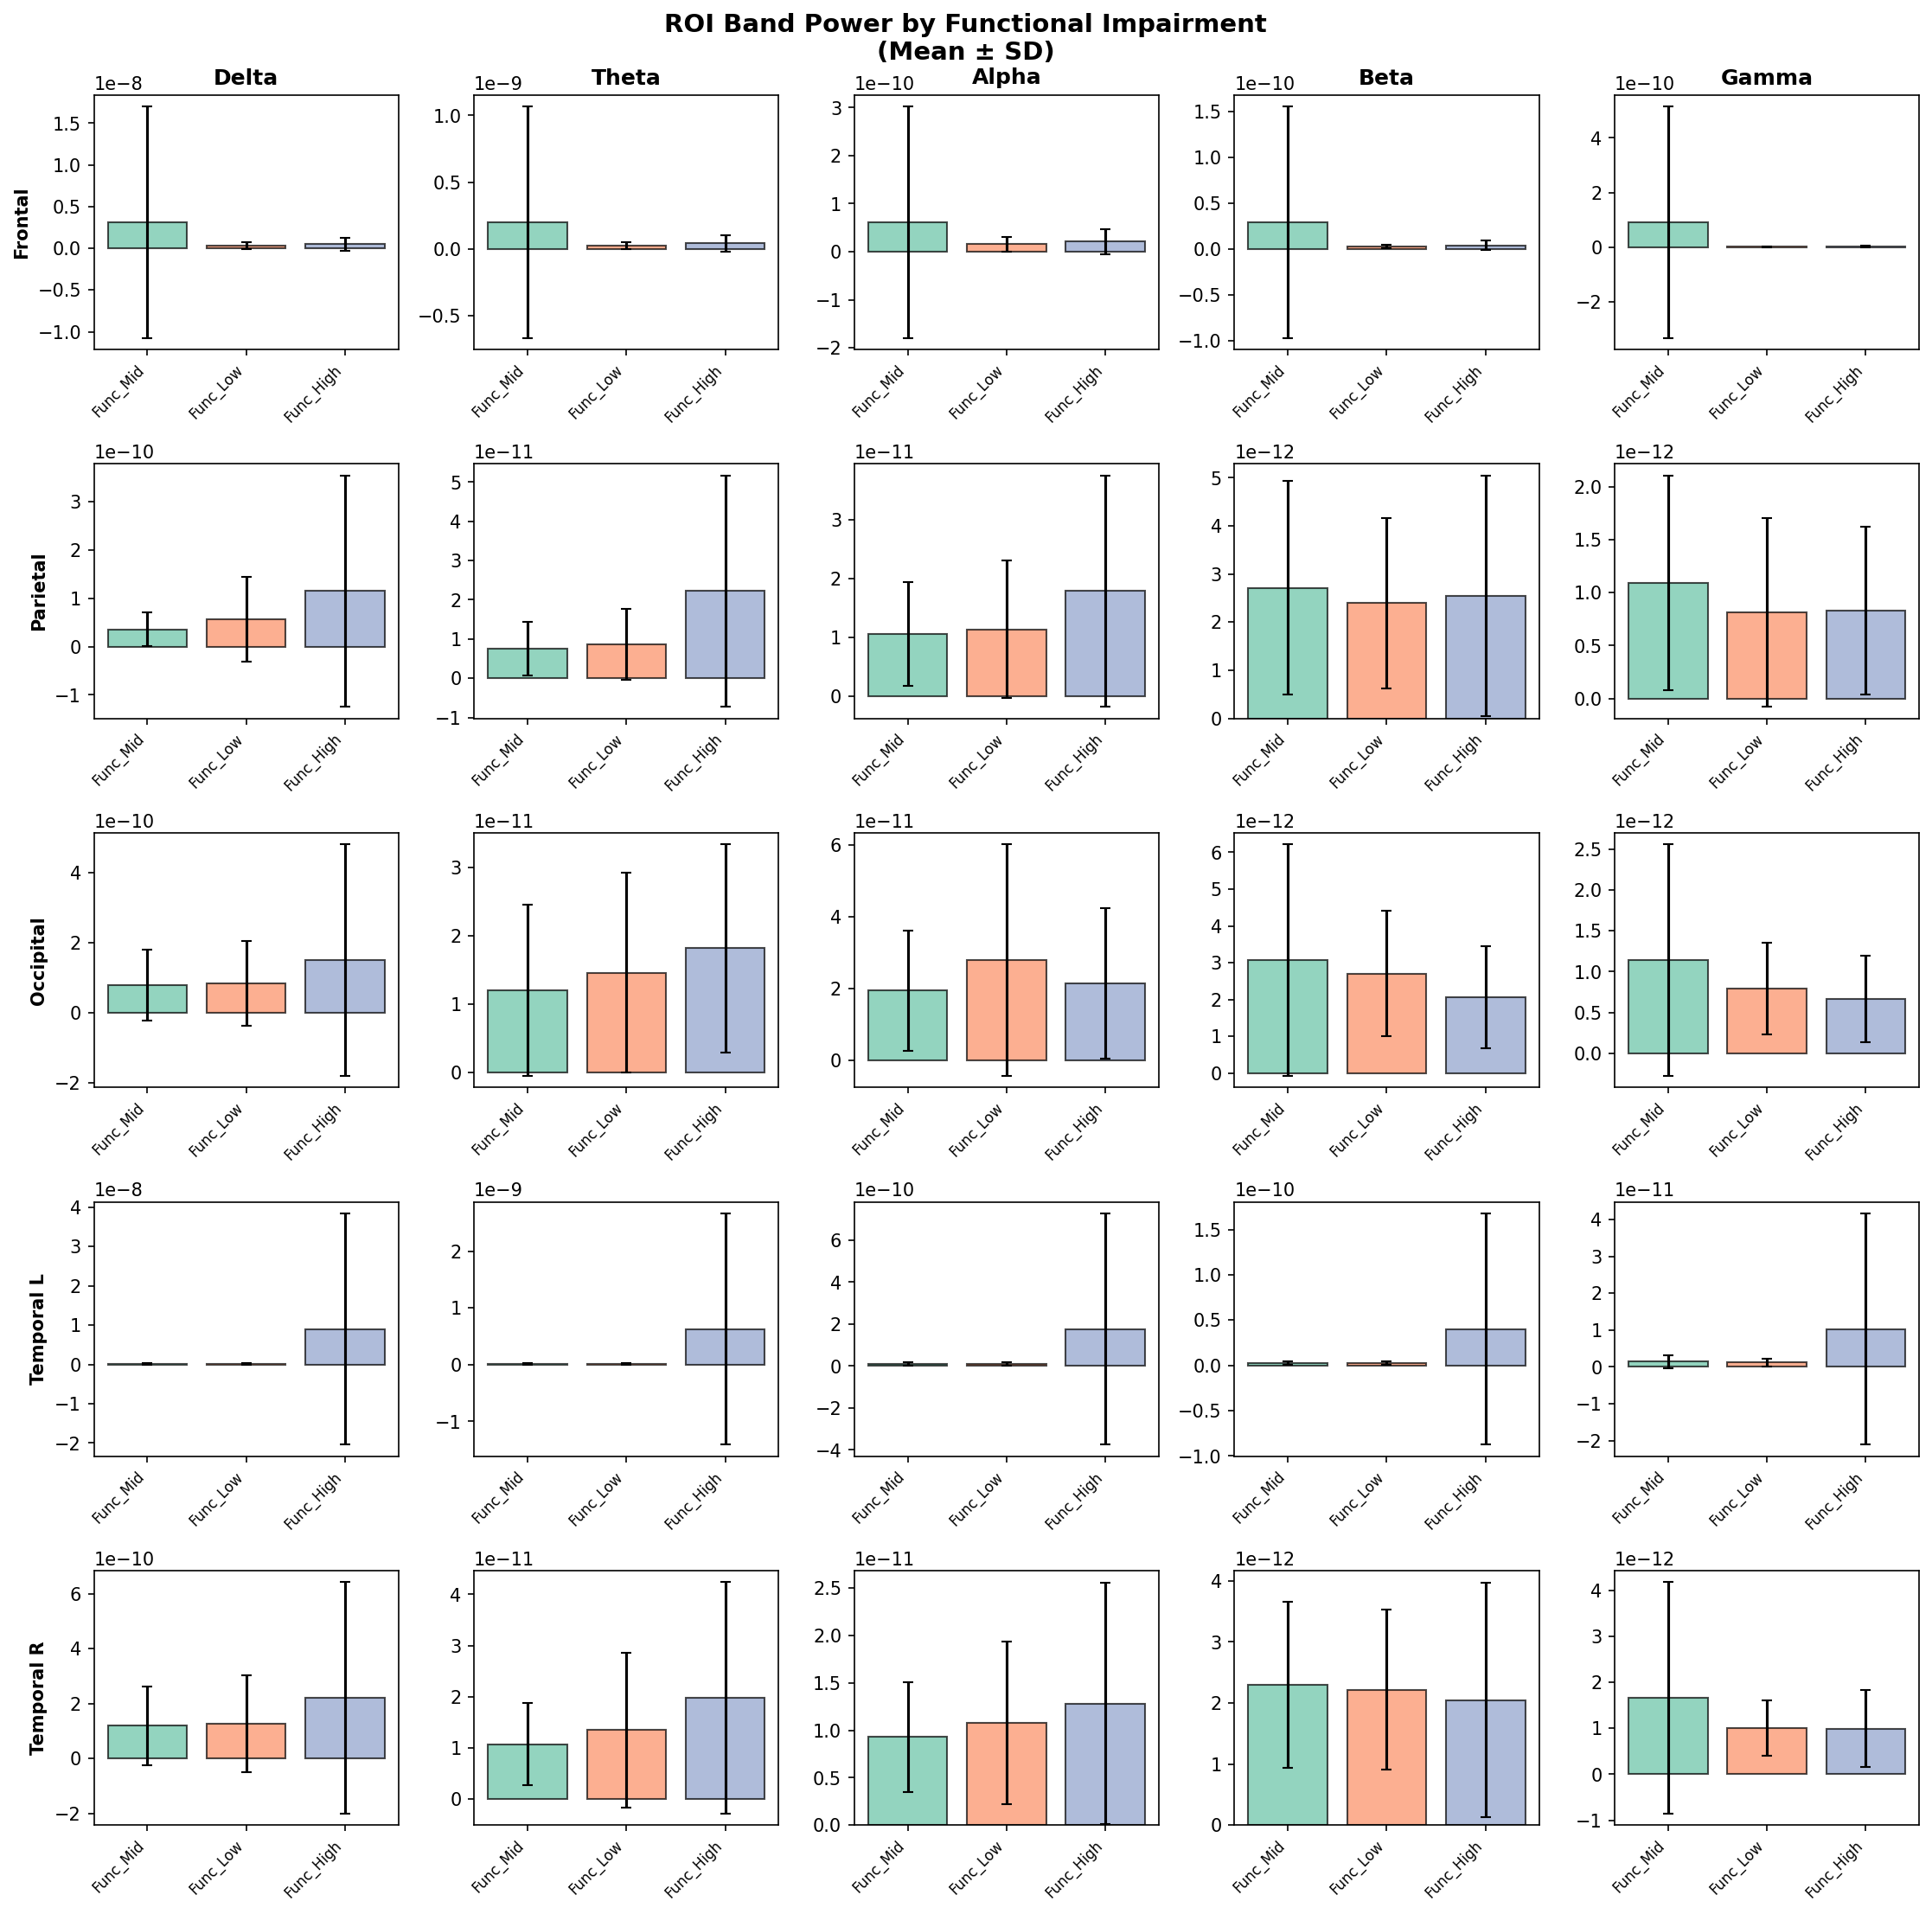
\includegraphics[width=\linewidth]{figures/paper2-wip/roi_power_comparison_functional_impairment.png}
    \caption{ROI power comparison by functional impairment.}
    \label{fig:roi_func}
\end{figure}

\subsection{Frontal-Posterior Asymmetry}

\begin{figure}[H]
    \centering
    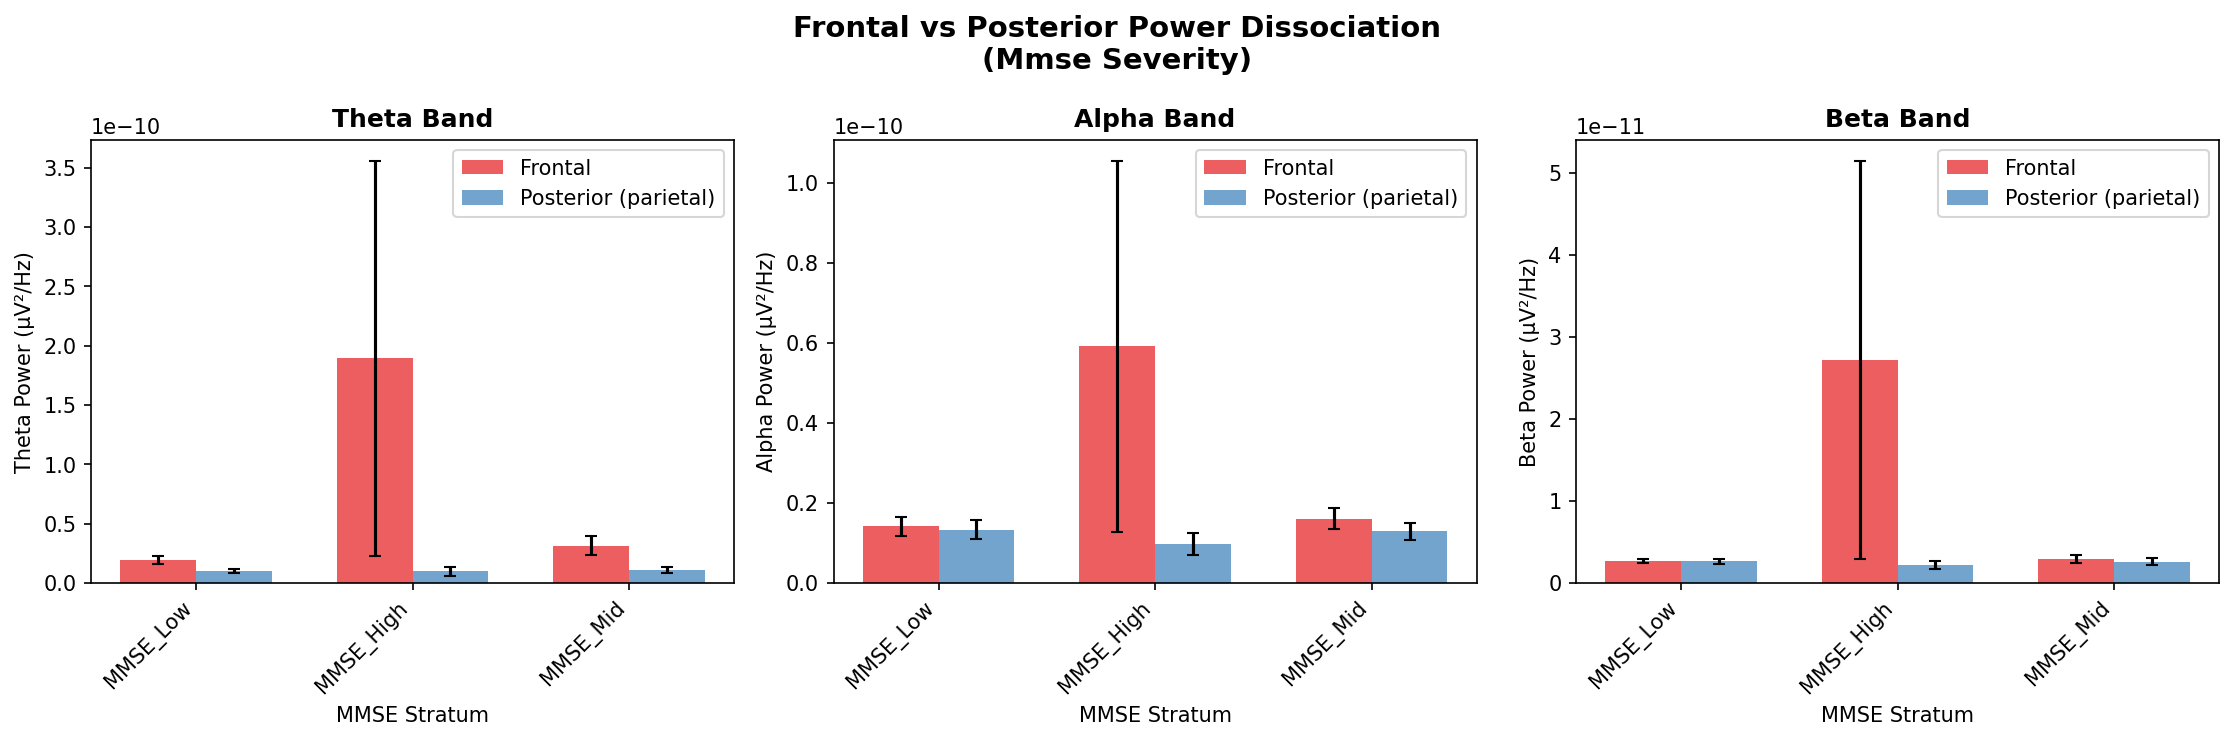
\includegraphics[width=\linewidth]{figures/paper2-wip/frontal_posterior_asymmetry_mmse_severity.png}
    \caption{Frontal-posterior power asymmetry by MMSE severity.}
    \label{fig:asymm_mmse}
\end{figure}

\begin{figure}[H]
    \centering
    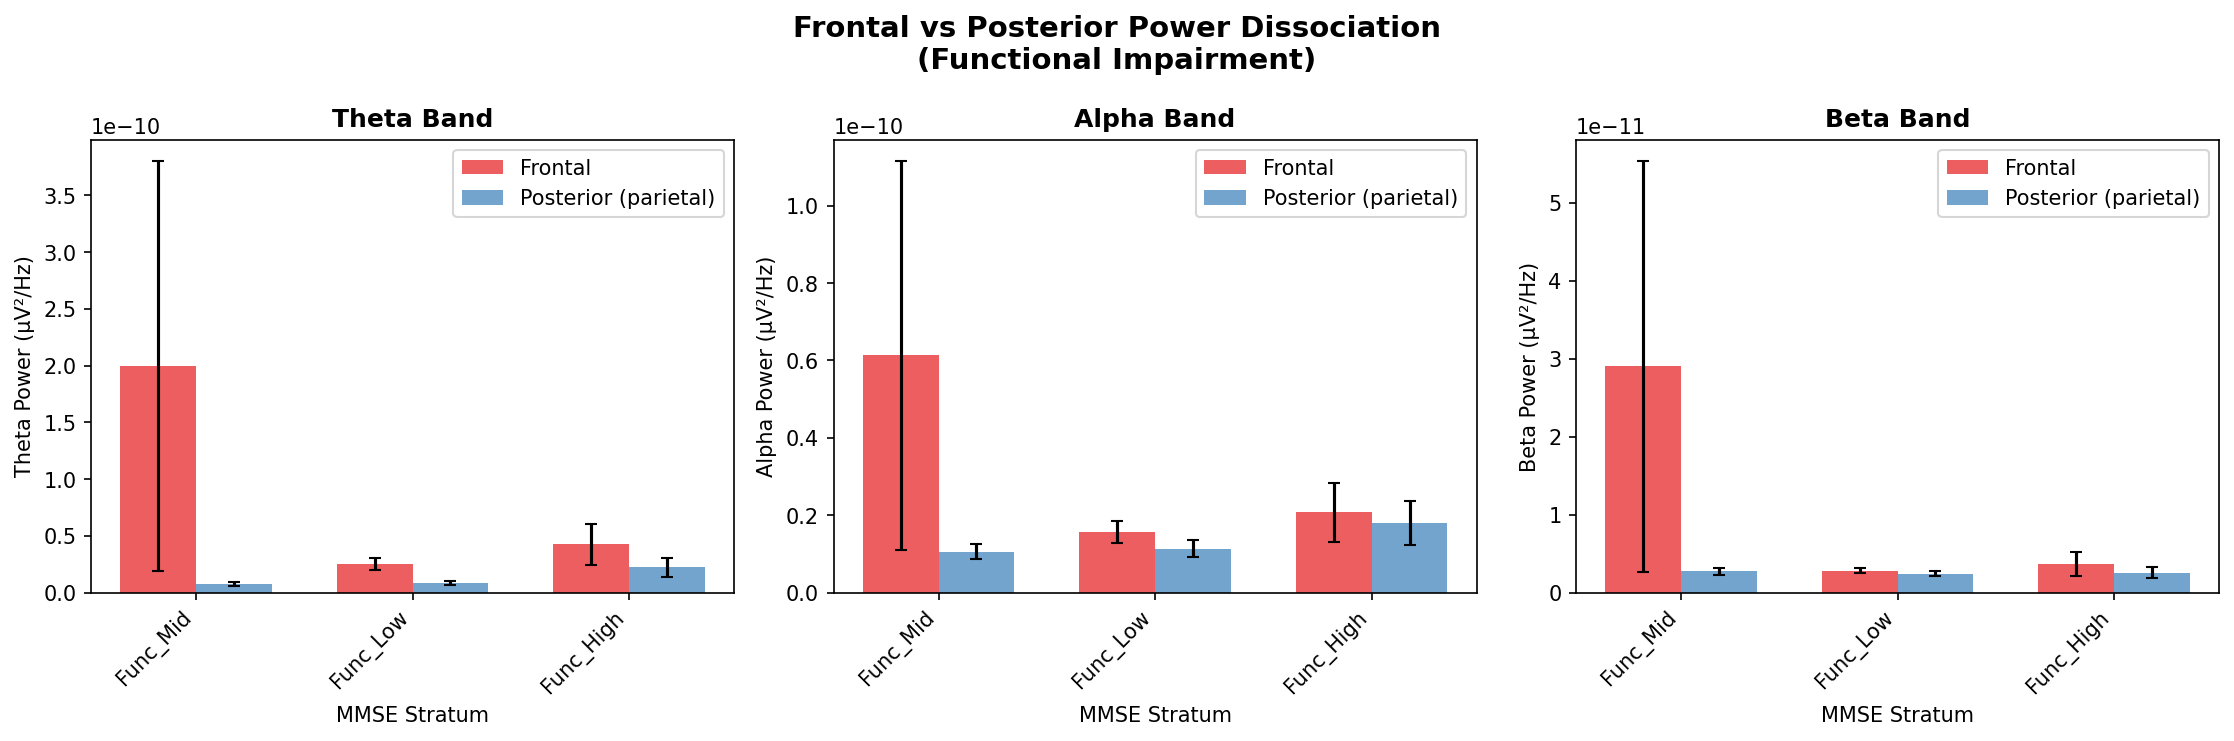
\includegraphics[width=\linewidth]{figures/paper2-wip/frontal_posterior_asymmetry_functional_impairment.png}
    \caption{Frontal-posterior power asymmetry by functional impairment.}
    \label{fig:asymm_func}
\end{figure}

% =========================
\section{Summary of Key Findings}
\label{sec:summary}
% =========================

\subsection{HC vs MCI vs AD}

\begin{enumerate}
    \item \textbf{MCI shows strongest dynamical alterations}: Large effect sizes for Speed CV ($d = -1.15$), Occupancy Entropy ($d = 1.14$), and Path Tortuosity ($d = 1.11$) distinguish MCI from HC.

    \item \textbf{AD shows reduced exploration}: Explored Variance is significantly reduced in AD vs HC ($d = 0.82$), but dynamics metrics (Speed CV, Tortuosity) are closer to HC values.

    \item \textbf{MCI has more variable, less complex dynamics}: Higher Speed CV and dramatically lower Path Tortuosity in MCI suggest more erratic but simpler trajectory patterns.

    \item \textbf{Spatial structure differs}: Flow field and density maps reveal group-specific occupancy patterns and flow organization.
\end{enumerate}

\subsection{MCI Subtypes}

\begin{enumerate}
    \item \textbf{MMSE severity modulates tortuosity}: Lower cognitive function (MMSE Low) associated with reduced Path Tortuosity ($d = -0.58$).

    \item \textbf{Functional impairment relates to speed}: Moderate functional impairment shows faster dynamics and more complex paths compared to severe impairment.

    \item \textbf{Subtype effects are smaller than diagnostic effects}: Within-MCI stratification shows effect sizes typically $|d| < 0.6$, compared to HC vs MCI effects of $|d| > 1.0$.
\end{enumerate}

\subsection{Interpretation}

The pattern of results suggests:
\begin{itemize}
    \item MCI may represent a state of \emph{dysregulated dynamics}---increased variability (Speed CV) but reduced complexity (Tortuosity) and exploration (Occupancy Entropy).

    \item AD shows \emph{reduced dynamic range} (Explored Variance) but more normalized local dynamics, possibly reflecting compensatory mechanisms or disease progression beyond the MCI stage.

    \item Within MCI, cognitive severity (MMSE) and functional status capture partially distinct aspects of dynamical organization.
\end{itemize}

% =========================
\section{Next Steps}
% =========================

\begin{enumerate}
    \item \textbf{HMM complementarity analysis}: Compare flow metrics to HMM-derived statistics to identify unique vs overlapping information.

    \item \textbf{Classification validation}: Test whether flow metrics improve subject-level classification beyond baseline features.

    \item \textbf{Longitudinal analysis}: If follow-up data available, examine whether baseline flow metrics predict conversion or decline.

    \item \textbf{Robustness checks}: Verify findings across different autoencoder architectures and preprocessing choices.
\end{enumerate}

\end{document}
